\documentclass[twoside]{book}

% Packages required by doxygen
\usepackage{fixltx2e}
\usepackage{calc}
\usepackage{doxygen}
\usepackage[export]{adjustbox} % also loads graphicx
\usepackage{graphicx}
\usepackage[utf8]{inputenc}
\usepackage{makeidx}
\usepackage{multicol}
\usepackage{multirow}
\PassOptionsToPackage{warn}{textcomp}
\usepackage{textcomp}
\usepackage[nointegrals]{wasysym}
\usepackage[table]{xcolor}

% Font selection
\usepackage[T1]{fontenc}
\usepackage[scaled=.90]{helvet}
\usepackage{courier}
\usepackage{amssymb}
\usepackage{sectsty}
\renewcommand{\familydefault}{\sfdefault}
\allsectionsfont{%
  \fontseries{bc}\selectfont%
  \color{darkgray}%
}
\renewcommand{\DoxyLabelFont}{%
  \fontseries{bc}\selectfont%
  \color{darkgray}%
}
\newcommand{\+}{\discretionary{\mbox{\scriptsize$\hookleftarrow$}}{}{}}

% Page & text layout
\usepackage{geometry}
\geometry{%
  a4paper,%
  top=2.5cm,%
  bottom=2.5cm,%
  left=2.5cm,%
  right=2.5cm%
}
\tolerance=750
\hfuzz=15pt
\hbadness=750
\setlength{\emergencystretch}{15pt}
\setlength{\parindent}{0cm}
\setlength{\parskip}{3ex plus 2ex minus 2ex}
\makeatletter
\renewcommand{\paragraph}{%
  \@startsection{paragraph}{4}{0ex}{-1.0ex}{1.0ex}{%
    \normalfont\normalsize\bfseries\SS@parafont%
  }%
}
\renewcommand{\subparagraph}{%
  \@startsection{subparagraph}{5}{0ex}{-1.0ex}{1.0ex}{%
    \normalfont\normalsize\bfseries\SS@subparafont%
  }%
}
\makeatother

% Headers & footers
\usepackage{fancyhdr}
\pagestyle{fancyplain}
\fancyhead[LE]{\fancyplain{}{\bfseries\thepage}}
\fancyhead[CE]{\fancyplain{}{}}
\fancyhead[RE]{\fancyplain{}{\bfseries\leftmark}}
\fancyhead[LO]{\fancyplain{}{\bfseries\rightmark}}
\fancyhead[CO]{\fancyplain{}{}}
\fancyhead[RO]{\fancyplain{}{\bfseries\thepage}}
\fancyfoot[LE]{\fancyplain{}{}}
\fancyfoot[CE]{\fancyplain{}{}}
\fancyfoot[RE]{\fancyplain{}{\bfseries\scriptsize Generated by Doxygen }}
\fancyfoot[LO]{\fancyplain{}{\bfseries\scriptsize Generated by Doxygen }}
\fancyfoot[CO]{\fancyplain{}{}}
\fancyfoot[RO]{\fancyplain{}{}}
\renewcommand{\footrulewidth}{0.4pt}
\renewcommand{\chaptermark}[1]{%
  \markboth{#1}{}%
}
\renewcommand{\sectionmark}[1]{%
  \markright{\thesection\ #1}%
}

% Indices & bibliography
\usepackage{natbib}
\usepackage[titles]{tocloft}
\setcounter{tocdepth}{3}
\setcounter{secnumdepth}{5}
\makeindex

% Hyperlinks (required, but should be loaded last)
\usepackage{ifpdf}
\ifpdf
  \usepackage[pdftex,pagebackref=true]{hyperref}
\else
  \usepackage[ps2pdf,pagebackref=true]{hyperref}
\fi
\hypersetup{%
  colorlinks=true,%
  linkcolor=blue,%
  citecolor=blue,%
  unicode%
}

% Custom commands
\newcommand{\clearemptydoublepage}{%
  \newpage{\pagestyle{empty}\cleardoublepage}%
}

\usepackage{caption}
\captionsetup{labelsep=space,justification=centering,font={bf},singlelinecheck=off,skip=4pt,position=top}

%===== C O N T E N T S =====

\begin{document}

% Titlepage & ToC
\hypersetup{pageanchor=false,
             bookmarksnumbered=true,
             pdfencoding=unicode
            }
\pagenumbering{alph}
\begin{titlepage}
\vspace*{7cm}
\begin{center}%
{\Large Mav\+Link\+Made\+Easy \\[1ex]\large 2.\+0 }\\
\vspace*{1cm}
{\large Generated by Doxygen 1.8.14}\\
\end{center}
\end{titlepage}
\clearemptydoublepage
\pagenumbering{roman}
\tableofcontents
\clearemptydoublepage
\pagenumbering{arabic}
\hypersetup{pageanchor=true}

%--- Begin generated contents ---
\chapter{L\+I\+C\+E\+N\+S\+E-\/\+S\+E\+L\+E\+C\+T2}
\label{md_mavAgenda_static_admin_css_vendor_select2_LICENSE-SELECT2}
\Hypertarget{md_mavAgenda_static_admin_css_vendor_select2_LICENSE-SELECT2}
The M\+IT License (M\+IT)

Copyright (c) 2012-\/2015 Kevin Brown, Igor Vaynberg, and Select2 contributors

Permission is hereby granted, free of charge, to any person obtaining a copy of this software and associated documentation files (the \char`\"{}\+Software\char`\"{}), to deal in the Software without restriction, including without limitation the rights to use, copy, modify, merge, publish, distribute, sublicense, and/or sell copies of the Software, and to permit persons to whom the Software is furnished to do so, subject to the following conditions\+:

The above copyright notice and this permission notice shall be included in all copies or substantial portions of the Software.

T\+HE S\+O\+F\+T\+W\+A\+RE IS P\+R\+O\+V\+I\+D\+ED \char`\"{}\+A\+S I\+S\char`\"{}, W\+I\+T\+H\+O\+UT W\+A\+R\+R\+A\+N\+TY OF A\+NY K\+I\+ND, E\+X\+P\+R\+E\+SS OR I\+M\+P\+L\+I\+ED, I\+N\+C\+L\+U\+D\+I\+NG B\+UT N\+OT L\+I\+M\+I\+T\+ED TO T\+HE W\+A\+R\+R\+A\+N\+T\+I\+ES OF M\+E\+R\+C\+H\+A\+N\+T\+A\+B\+I\+L\+I\+TY, F\+I\+T\+N\+E\+SS F\+OR A P\+A\+R\+T\+I\+C\+U\+L\+AR P\+U\+R\+P\+O\+SE A\+ND N\+O\+N\+I\+N\+F\+R\+I\+N\+G\+E\+M\+E\+NT. IN NO E\+V\+E\+NT S\+H\+A\+LL T\+HE A\+U\+T\+H\+O\+RS OR C\+O\+P\+Y\+R\+I\+G\+HT H\+O\+L\+D\+E\+RS BE L\+I\+A\+B\+LE F\+OR A\+NY C\+L\+A\+IM, D\+A\+M\+A\+G\+ES OR O\+T\+H\+ER L\+I\+A\+B\+I\+L\+I\+TY, W\+H\+E\+T\+H\+ER IN AN A\+C\+T\+I\+ON OF C\+O\+N\+T\+R\+A\+CT, T\+O\+RT OR O\+T\+H\+E\+R\+W\+I\+SE, A\+R\+I\+S\+I\+NG F\+R\+OM, O\+UT OF OR IN C\+O\+N\+N\+E\+C\+T\+I\+ON W\+I\+TH T\+HE S\+O\+F\+T\+W\+A\+RE OR T\+HE U\+SE OR O\+T\+H\+ER D\+E\+A\+L\+I\+N\+GS IN T\+HE S\+O\+F\+T\+W\+A\+RE. 
\chapter{L\+I\+C\+E\+N\+S\+E-\/\+S\+E\+L\+E\+C\+T2}
\label{md_mavAgenda_static_admin_js_vendor_select2_LICENSE-SELECT2}
\Hypertarget{md_mavAgenda_static_admin_js_vendor_select2_LICENSE-SELECT2}
The M\+IT License (M\+IT)

Copyright (c) 2012-\/2015 Kevin Brown, Igor Vaynberg, and Select2 contributors

Permission is hereby granted, free of charge, to any person obtaining a copy of this software and associated documentation files (the \char`\"{}\+Software\char`\"{}), to deal in the Software without restriction, including without limitation the rights to use, copy, modify, merge, publish, distribute, sublicense, and/or sell copies of the Software, and to permit persons to whom the Software is furnished to do so, subject to the following conditions\+:

The above copyright notice and this permission notice shall be included in all copies or substantial portions of the Software.

T\+HE S\+O\+F\+T\+W\+A\+RE IS P\+R\+O\+V\+I\+D\+ED \char`\"{}\+A\+S I\+S\char`\"{}, W\+I\+T\+H\+O\+UT W\+A\+R\+R\+A\+N\+TY OF A\+NY K\+I\+ND, E\+X\+P\+R\+E\+SS OR I\+M\+P\+L\+I\+ED, I\+N\+C\+L\+U\+D\+I\+NG B\+UT N\+OT L\+I\+M\+I\+T\+ED TO T\+HE W\+A\+R\+R\+A\+N\+T\+I\+ES OF M\+E\+R\+C\+H\+A\+N\+T\+A\+B\+I\+L\+I\+TY, F\+I\+T\+N\+E\+SS F\+OR A P\+A\+R\+T\+I\+C\+U\+L\+AR P\+U\+R\+P\+O\+SE A\+ND N\+O\+N\+I\+N\+F\+R\+I\+N\+G\+E\+M\+E\+NT. IN NO E\+V\+E\+NT S\+H\+A\+LL T\+HE A\+U\+T\+H\+O\+RS OR C\+O\+P\+Y\+R\+I\+G\+HT H\+O\+L\+D\+E\+RS BE L\+I\+A\+B\+LE F\+OR A\+NY C\+L\+A\+IM, D\+A\+M\+A\+G\+ES OR O\+T\+H\+ER L\+I\+A\+B\+I\+L\+I\+TY, W\+H\+E\+T\+H\+ER IN AN A\+C\+T\+I\+ON OF C\+O\+N\+T\+R\+A\+CT, T\+O\+RT OR O\+T\+H\+E\+R\+W\+I\+SE, A\+R\+I\+S\+I\+NG F\+R\+OM, O\+UT OF OR IN C\+O\+N\+N\+E\+C\+T\+I\+ON W\+I\+TH T\+HE S\+O\+F\+T\+W\+A\+RE OR T\+HE U\+SE OR O\+T\+H\+ER D\+E\+A\+L\+I\+N\+GS IN T\+HE S\+O\+F\+T\+W\+A\+RE. 
\chapter{Mav\+Link\+Made\+Easy}
\label{md_README}
\Hypertarget{md_README}
Summer 2018-\/ C\+S\+CI 4830-\/860 Software Engineering\+: Project Party 
\chapter{Namespace Index}
\section{Namespace List}
Here is a list of all namespaces with brief descriptions\+:\begin{DoxyCompactList}
\item\contentsline{section}{\mbox{\hyperlink{namespacelanding}{landing}} }{\pageref{namespacelanding}}{}
\item\contentsline{section}{\mbox{\hyperlink{namespacelanding_1_1admin}{landing.\+admin}} }{\pageref{namespacelanding_1_1admin}}{}
\item\contentsline{section}{\mbox{\hyperlink{namespacelanding_1_1apps}{landing.\+apps}} }{\pageref{namespacelanding_1_1apps}}{}
\item\contentsline{section}{\mbox{\hyperlink{namespacelanding_1_1forms}{landing.\+forms}} }{\pageref{namespacelanding_1_1forms}}{}
\item\contentsline{section}{\mbox{\hyperlink{namespacelanding_1_1migrations}{landing.\+migrations}} }{\pageref{namespacelanding_1_1migrations}}{}
\item\contentsline{section}{\mbox{\hyperlink{namespacelanding_1_1migrations_1_10001__initial}{landing.\+migrations.\+0001\+\_\+initial}} }{\pageref{namespacelanding_1_1migrations_1_10001__initial}}{}
\item\contentsline{section}{\mbox{\hyperlink{namespacelanding_1_1models}{landing.\+models}} }{\pageref{namespacelanding_1_1models}}{}
\item\contentsline{section}{\mbox{\hyperlink{namespacelanding_1_1tests}{landing.\+tests}} }{\pageref{namespacelanding_1_1tests}}{}
\item\contentsline{section}{\mbox{\hyperlink{namespacelanding_1_1tests_1_1test__logic}{landing.\+tests.\+test\+\_\+logic}} }{\pageref{namespacelanding_1_1tests_1_1test__logic}}{}
\item\contentsline{section}{\mbox{\hyperlink{namespacelanding_1_1tests_1_1test__UI}{landing.\+tests.\+test\+\_\+\+UI}} }{\pageref{namespacelanding_1_1tests_1_1test__UI}}{}
\item\contentsline{section}{\mbox{\hyperlink{namespacelanding_1_1urls}{landing.\+urls}} }{\pageref{namespacelanding_1_1urls}}{}
\item\contentsline{section}{\mbox{\hyperlink{namespacelanding_1_1views}{landing.\+views}} }{\pageref{namespacelanding_1_1views}}{}
\item\contentsline{section}{\mbox{\hyperlink{namespacemanage}{manage}} }{\pageref{namespacemanage}}{}
\item\contentsline{section}{\mbox{\hyperlink{namespacemavAgenda}{mav\+Agenda}} }{\pageref{namespacemavAgenda}}{}
\item\contentsline{section}{\mbox{\hyperlink{namespacemavAgenda_1_1settings}{mav\+Agenda.\+settings}} }{\pageref{namespacemavAgenda_1_1settings}}{}
\item\contentsline{section}{\mbox{\hyperlink{namespacemavAgenda_1_1urls}{mav\+Agenda.\+urls}} }{\pageref{namespacemavAgenda_1_1urls}}{}
\item\contentsline{section}{\mbox{\hyperlink{namespacemavAgenda_1_1views}{mav\+Agenda.\+views}} }{\pageref{namespacemavAgenda_1_1views}}{}
\item\contentsline{section}{\mbox{\hyperlink{namespacemavAgenda_1_1wsgi}{mav\+Agenda.\+wsgi}} }{\pageref{namespacemavAgenda_1_1wsgi}}{}
\item\contentsline{section}{\mbox{\hyperlink{namespacescrape}{scrape}} }{\pageref{namespacescrape}}{}
\item\contentsline{section}{\mbox{\hyperlink{namespacetemplates}{templates}} }{\pageref{namespacetemplates}}{}
\item\contentsline{section}{\mbox{\hyperlink{namespacetest}{test}} }{\pageref{namespacetest}}{}
\end{DoxyCompactList}

\chapter{Hierarchical Index}
\section{Class Hierarchy}
This inheritance list is sorted roughly, but not completely, alphabetically\+:\begin{DoxyCompactList}
\item \contentsline{section}{landing.\+forms.\+User\+Form.\+Meta}{\pageref{classlanding_1_1forms_1_1UserForm_1_1Meta}}{}
\item Migration\begin{DoxyCompactList}
\item \contentsline{section}{landing.\+migrations.0001\+\_\+initial.Migration}{\pageref{classlanding_1_1migrations_1_10001__initial_1_1Migration}}{}
\end{DoxyCompactList}
\item Model\begin{DoxyCompactList}
\item \contentsline{section}{landing.\+models.\+Building}{\pageref{classlanding_1_1models_1_1Building}}{}
\item \contentsline{section}{landing.\+models.\+Campus}{\pageref{classlanding_1_1models_1_1Campus}}{}
\item \contentsline{section}{landing.\+models.\+Complete}{\pageref{classlanding_1_1models_1_1Complete}}{}
\item \contentsline{section}{landing.\+models.\+Course}{\pageref{classlanding_1_1models_1_1Course}}{}
\item \contentsline{section}{landing.\+models.\+Degree}{\pageref{classlanding_1_1models_1_1Degree}}{}
\item \contentsline{section}{landing.\+models.\+Instructor}{\pageref{classlanding_1_1models_1_1Instructor}}{}
\item \contentsline{section}{landing.\+models.\+Offering}{\pageref{classlanding_1_1models_1_1Offering}}{}
\item \contentsline{section}{landing.\+models.\+Prereq}{\pageref{classlanding_1_1models_1_1Prereq}}{}
\item \contentsline{section}{landing.\+models.\+Requirement}{\pageref{classlanding_1_1models_1_1Requirement}}{}
\item \contentsline{section}{landing.\+models.\+User\+Preferences}{\pageref{classlanding_1_1models_1_1UserPreferences}}{}
\item \contentsline{section}{landing.\+models.\+Weekday}{\pageref{classlanding_1_1models_1_1Weekday}}{}
\end{DoxyCompactList}
\item Model\+Form\begin{DoxyCompactList}
\item \contentsline{section}{landing.\+forms.\+User\+Form}{\pageref{classlanding_1_1forms_1_1UserForm}}{}
\end{DoxyCompactList}
\item App\+Config\begin{DoxyCompactList}
\item \contentsline{section}{landing.\+apps.\+Landing\+Config}{\pageref{classlanding_1_1apps_1_1LandingConfig}}{}
\end{DoxyCompactList}
\item Static\+Live\+Server\+Test\+Case\begin{DoxyCompactList}
\item \contentsline{section}{landing.\+tests.\+test\+\_\+\+U\+I.\+U\+I\+Tests}{\pageref{classlanding_1_1tests_1_1test__UI_1_1UITests}}{}
\end{DoxyCompactList}
\item Test\+Case\begin{DoxyCompactList}
\item \contentsline{section}{landing.\+tests.\+test\+\_\+logic.\+Your\+Test\+Class}{\pageref{classlanding_1_1tests_1_1test__logic_1_1YourTestClass}}{}
\end{DoxyCompactList}
\end{DoxyCompactList}

\chapter{Class Index}
\section{Class List}
Here are the classes, structs, unions and interfaces with brief descriptions\+:\begin{DoxyCompactList}
\item\contentsline{section}{\mbox{\hyperlink{classlanding_1_1models_1_1Building}{landing.\+models.\+Building}} }{\pageref{classlanding_1_1models_1_1Building}}{}
\item\contentsline{section}{\mbox{\hyperlink{classlanding_1_1models_1_1Campus}{landing.\+models.\+Campus}} }{\pageref{classlanding_1_1models_1_1Campus}}{}
\item\contentsline{section}{\mbox{\hyperlink{classlanding_1_1models_1_1Complete}{landing.\+models.\+Complete}} }{\pageref{classlanding_1_1models_1_1Complete}}{}
\item\contentsline{section}{\mbox{\hyperlink{classlanding_1_1models_1_1Course}{landing.\+models.\+Course}} }{\pageref{classlanding_1_1models_1_1Course}}{}
\item\contentsline{section}{\mbox{\hyperlink{classlanding_1_1models_1_1Degree}{landing.\+models.\+Degree}} }{\pageref{classlanding_1_1models_1_1Degree}}{}
\item\contentsline{section}{\mbox{\hyperlink{classlanding_1_1models_1_1Instructor}{landing.\+models.\+Instructor}} }{\pageref{classlanding_1_1models_1_1Instructor}}{}
\item\contentsline{section}{\mbox{\hyperlink{classlanding_1_1apps_1_1LandingConfig}{landing.\+apps.\+Landing\+Config}} }{\pageref{classlanding_1_1apps_1_1LandingConfig}}{}
\item\contentsline{section}{\mbox{\hyperlink{classlanding_1_1forms_1_1UserForm_1_1Meta}{landing.\+forms.\+User\+Form.\+Meta}} }{\pageref{classlanding_1_1forms_1_1UserForm_1_1Meta}}{}
\item\contentsline{section}{\mbox{\hyperlink{classlanding_1_1migrations_1_10001__initial_1_1Migration}{landing.\+migrations.\+0001\+\_\+initial.\+Migration}} }{\pageref{classlanding_1_1migrations_1_10001__initial_1_1Migration}}{}
\item\contentsline{section}{\mbox{\hyperlink{classlanding_1_1models_1_1Offering}{landing.\+models.\+Offering}} }{\pageref{classlanding_1_1models_1_1Offering}}{}
\item\contentsline{section}{\mbox{\hyperlink{classlanding_1_1models_1_1Prereq}{landing.\+models.\+Prereq}} }{\pageref{classlanding_1_1models_1_1Prereq}}{}
\item\contentsline{section}{\mbox{\hyperlink{classlanding_1_1models_1_1Requirement}{landing.\+models.\+Requirement}} }{\pageref{classlanding_1_1models_1_1Requirement}}{}
\item\contentsline{section}{\mbox{\hyperlink{classlanding_1_1tests_1_1test__UI_1_1UITests}{landing.\+tests.\+test\+\_\+\+U\+I.\+U\+I\+Tests}} }{\pageref{classlanding_1_1tests_1_1test__UI_1_1UITests}}{}
\item\contentsline{section}{\mbox{\hyperlink{classlanding_1_1forms_1_1UserForm}{landing.\+forms.\+User\+Form}} }{\pageref{classlanding_1_1forms_1_1UserForm}}{}
\item\contentsline{section}{\mbox{\hyperlink{classlanding_1_1models_1_1UserPreferences}{landing.\+models.\+User\+Preferences}} }{\pageref{classlanding_1_1models_1_1UserPreferences}}{}
\item\contentsline{section}{\mbox{\hyperlink{classlanding_1_1models_1_1Weekday}{landing.\+models.\+Weekday}} }{\pageref{classlanding_1_1models_1_1Weekday}}{}
\item\contentsline{section}{\mbox{\hyperlink{classlanding_1_1tests_1_1test__logic_1_1YourTestClass}{landing.\+tests.\+test\+\_\+logic.\+Your\+Test\+Class}} }{\pageref{classlanding_1_1tests_1_1test__logic_1_1YourTestClass}}{}
\end{DoxyCompactList}

\chapter{File Index}
\section{File List}
Here is a list of all files with brief descriptions\+:\begin{DoxyCompactList}
\item\contentsline{section}{\mbox{\hyperlink{test_8py}{test.\+py}} }{\pageref{test_8py}}{}
\item\contentsline{section}{matriculation\+Utility/\mbox{\hyperlink{scrape_8py}{scrape.\+py}} }{\pageref{scrape_8py}}{}
\item\contentsline{section}{mav\+Agenda/\mbox{\hyperlink{manage_8py}{manage.\+py}} }{\pageref{manage_8py}}{}
\item\contentsline{section}{mav\+Agenda/landing/\mbox{\hyperlink{landing_2____init_____8py}{\+\_\+\+\_\+init\+\_\+\+\_\+.\+py}} }{\pageref{landing_2____init_____8py}}{}
\item\contentsline{section}{mav\+Agenda/landing/\mbox{\hyperlink{admin_8py}{admin.\+py}} }{\pageref{admin_8py}}{}
\item\contentsline{section}{mav\+Agenda/landing/\mbox{\hyperlink{apps_8py}{apps.\+py}} }{\pageref{apps_8py}}{}
\item\contentsline{section}{mav\+Agenda/landing/\mbox{\hyperlink{forms_8py}{forms.\+py}} }{\pageref{forms_8py}}{}
\item\contentsline{section}{mav\+Agenda/landing/\mbox{\hyperlink{models_8py}{models.\+py}} }{\pageref{models_8py}}{}
\item\contentsline{section}{mav\+Agenda/landing/\mbox{\hyperlink{landing_2urls_8py}{urls.\+py}} }{\pageref{landing_2urls_8py}}{}
\item\contentsline{section}{mav\+Agenda/landing/\mbox{\hyperlink{landing_2views_8py}{views.\+py}} }{\pageref{landing_2views_8py}}{}
\item\contentsline{section}{mav\+Agenda/landing/migrations/\mbox{\hyperlink{0001__initial_8py}{0001\+\_\+initial.\+py}} }{\pageref{0001__initial_8py}}{}
\item\contentsline{section}{mav\+Agenda/landing/migrations/\mbox{\hyperlink{landing_2migrations_2____init_____8py}{\+\_\+\+\_\+init\+\_\+\+\_\+.\+py}} }{\pageref{landing_2migrations_2____init_____8py}}{}
\item\contentsline{section}{mav\+Agenda/landing/templates/landing/\mbox{\hyperlink{base_8html}{base.\+html}} }{\pageref{base_8html}}{}
\item\contentsline{section}{mav\+Agenda/landing/templates/landing/\mbox{\hyperlink{createuser_8html}{createuser.\+html}} }{\pageref{createuser_8html}}{}
\item\contentsline{section}{mav\+Agenda/landing/templates/landing/\mbox{\hyperlink{login_8html}{login.\+html}} }{\pageref{login_8html}}{}
\item\contentsline{section}{mav\+Agenda/landing/templates/landing/\mbox{\hyperlink{nextsemesterpreferences_8html}{nextsemesterpreferences.\+html}} }{\pageref{nextsemesterpreferences_8html}}{}
\item\contentsline{section}{mav\+Agenda/landing/templates/landing/\mbox{\hyperlink{schedule_8html}{schedule.\+html}} }{\pageref{schedule_8html}}{}
\item\contentsline{section}{mav\+Agenda/landing/templates/landing/\mbox{\hyperlink{selectcourses_8html}{selectcourses.\+html}} }{\pageref{selectcourses_8html}}{}
\item\contentsline{section}{mav\+Agenda/landing/tests/\mbox{\hyperlink{landing_2tests_2____init_____8py}{\+\_\+\+\_\+init\+\_\+\+\_\+.\+py}} }{\pageref{landing_2tests_2____init_____8py}}{}
\item\contentsline{section}{mav\+Agenda/landing/tests/\mbox{\hyperlink{test__logic_8py}{test\+\_\+logic.\+py}} }{\pageref{test__logic_8py}}{}
\item\contentsline{section}{mav\+Agenda/landing/tests/\mbox{\hyperlink{test__UI_8py}{test\+\_\+\+U\+I.\+py}} }{\pageref{test__UI_8py}}{}
\item\contentsline{section}{mav\+Agenda/mav\+Agenda/\mbox{\hyperlink{mavAgenda_2____init_____8py}{\+\_\+\+\_\+init\+\_\+\+\_\+.\+py}} }{\pageref{mavAgenda_2____init_____8py}}{}
\item\contentsline{section}{mav\+Agenda/mav\+Agenda/\mbox{\hyperlink{settings_8py}{settings.\+py}} }{\pageref{settings_8py}}{}
\item\contentsline{section}{mav\+Agenda/mav\+Agenda/\mbox{\hyperlink{mavAgenda_2urls_8py}{urls.\+py}} }{\pageref{mavAgenda_2urls_8py}}{}
\item\contentsline{section}{mav\+Agenda/mav\+Agenda/\mbox{\hyperlink{mavAgenda_2views_8py}{views.\+py}} }{\pageref{mavAgenda_2views_8py}}{}
\item\contentsline{section}{mav\+Agenda/mav\+Agenda/\mbox{\hyperlink{wsgi_8py}{wsgi.\+py}} }{\pageref{wsgi_8py}}{}
\item\contentsline{section}{mav\+Agenda/static/admin/css/\mbox{\hyperlink{autocomplete_8css}{autocomplete.\+css}} }{\pageref{autocomplete_8css}}{}
\item\contentsline{section}{mav\+Agenda/static/admin/css/\mbox{\hyperlink{base_8css}{base.\+css}} }{\pageref{base_8css}}{}
\item\contentsline{section}{mav\+Agenda/static/admin/css/\mbox{\hyperlink{changelists_8css}{changelists.\+css}} }{\pageref{changelists_8css}}{}
\item\contentsline{section}{mav\+Agenda/static/admin/css/\mbox{\hyperlink{dashboard_8css}{dashboard.\+css}} }{\pageref{dashboard_8css}}{}
\item\contentsline{section}{mav\+Agenda/static/admin/css/\mbox{\hyperlink{fonts_8css}{fonts.\+css}} }{\pageref{fonts_8css}}{}
\item\contentsline{section}{mav\+Agenda/static/admin/css/\mbox{\hyperlink{forms_8css}{forms.\+css}} }{\pageref{forms_8css}}{}
\item\contentsline{section}{mav\+Agenda/static/admin/css/\mbox{\hyperlink{landing_8css}{landing.\+css}} }{\pageref{landing_8css}}{}
\item\contentsline{section}{mav\+Agenda/static/admin/css/\mbox{\hyperlink{login_8css}{login.\+css}} }{\pageref{login_8css}}{}
\item\contentsline{section}{mav\+Agenda/static/admin/css/\mbox{\hyperlink{responsive_8css}{responsive.\+css}} }{\pageref{responsive_8css}}{}
\item\contentsline{section}{mav\+Agenda/static/admin/css/\mbox{\hyperlink{responsive__rtl_8css}{responsive\+\_\+rtl.\+css}} }{\pageref{responsive__rtl_8css}}{}
\item\contentsline{section}{mav\+Agenda/static/admin/css/\mbox{\hyperlink{rtl_8css}{rtl.\+css}} }{\pageref{rtl_8css}}{}
\item\contentsline{section}{mav\+Agenda/static/admin/css/\mbox{\hyperlink{widgets_8css}{widgets.\+css}} }{\pageref{widgets_8css}}{}
\item\contentsline{section}{mav\+Agenda/static/admin/css/vendor/select2/\mbox{\hyperlink{select2_8css}{select2.\+css}} }{\pageref{select2_8css}}{}
\item\contentsline{section}{mav\+Agenda/static/admin/css/vendor/select2/\mbox{\hyperlink{select2_8min_8css}{select2.\+min.\+css}} }{\pageref{select2_8min_8css}}{}
\item\contentsline{section}{mav\+Agenda/static/landing/css/\mbox{\hyperlink{style_8css}{style.\+css}} }{\pageref{style_8css}}{}
\item\contentsline{section}{mav\+Agenda/templates/\mbox{\hyperlink{templates_2____init_____8py}{\+\_\+\+\_\+init\+\_\+\+\_\+.\+py}} }{\pageref{templates_2____init_____8py}}{}
\end{DoxyCompactList}

\chapter{Namespace Documentation}
\hypertarget{namespacelanding}{}\section{landing Namespace Reference}
\label{namespacelanding}\index{landing@{landing}}
\subsection*{Namespaces}
\begin{DoxyCompactItemize}
\item 
 \mbox{\hyperlink{namespacelanding_1_1admin}{admin}}
\item 
 \mbox{\hyperlink{namespacelanding_1_1apps}{apps}}
\item 
 \mbox{\hyperlink{namespacelanding_1_1forms}{forms}}
\item 
 \mbox{\hyperlink{namespacelanding_1_1migrations}{migrations}}
\item 
 \mbox{\hyperlink{namespacelanding_1_1models}{models}}
\item 
 \mbox{\hyperlink{namespacelanding_1_1tests}{tests}}
\item 
 \mbox{\hyperlink{namespacelanding_1_1urls}{urls}}
\item 
 \mbox{\hyperlink{namespacelanding_1_1views}{views}}
\end{DoxyCompactItemize}

\hypertarget{namespacelanding_1_1admin}{}\section{landing.\+admin Namespace Reference}
\label{namespacelanding_1_1admin}\index{landing.\+admin@{landing.\+admin}}

\hypertarget{namespacelanding_1_1apps}{}\section{landing.\+apps Namespace Reference}
\label{namespacelanding_1_1apps}\index{landing.\+apps@{landing.\+apps}}
\subsection*{Classes}
\begin{DoxyCompactItemize}
\item 
class \mbox{\hyperlink{classlanding_1_1apps_1_1LandingConfig}{Landing\+Config}}
\end{DoxyCompactItemize}

\hypertarget{namespacelanding_1_1forms}{}\section{landing.\+forms Namespace Reference}
\label{namespacelanding_1_1forms}\index{landing.\+forms@{landing.\+forms}}
\subsection*{Classes}
\begin{DoxyCompactItemize}
\item 
class \mbox{\hyperlink{classlanding_1_1forms_1_1UserForm}{User\+Form}}
\end{DoxyCompactItemize}

\hypertarget{namespacelanding_1_1migrations}{}\section{landing.\+migrations Namespace Reference}
\label{namespacelanding_1_1migrations}\index{landing.\+migrations@{landing.\+migrations}}
\subsection*{Namespaces}
\begin{DoxyCompactItemize}
\item 
 \mbox{\hyperlink{namespacelanding_1_1migrations_1_10001__initial}{0001\+\_\+initial}}
\end{DoxyCompactItemize}

\hypertarget{namespacelanding_1_1migrations_1_10001__initial}{}\section{landing.\+migrations.0001\+\_\+initial Namespace Reference}
\label{namespacelanding_1_1migrations_1_10001__initial}\index{landing.\+migrations.\+0001\+\_\+initial@{landing.\+migrations.\+0001\+\_\+initial}}
\subsection*{Classes}
\begin{DoxyCompactItemize}
\item 
class \mbox{\hyperlink{classlanding_1_1migrations_1_10001__initial_1_1Migration}{Migration}}
\end{DoxyCompactItemize}

\hypertarget{namespacelanding_1_1models}{}\section{landing.\+models Namespace Reference}
\label{namespacelanding_1_1models}\index{landing.\+models@{landing.\+models}}
\subsection*{Classes}
\begin{DoxyCompactItemize}
\item 
class \mbox{\hyperlink{classlanding_1_1models_1_1Building}{Building}}
\item 
class \mbox{\hyperlink{classlanding_1_1models_1_1Campus}{Campus}}
\item 
class \mbox{\hyperlink{classlanding_1_1models_1_1Complete}{Complete}}
\item 
class \mbox{\hyperlink{classlanding_1_1models_1_1Course}{Course}}
\item 
class \mbox{\hyperlink{classlanding_1_1models_1_1Degree}{Degree}}
\item 
class \mbox{\hyperlink{classlanding_1_1models_1_1Instructor}{Instructor}}
\item 
class \mbox{\hyperlink{classlanding_1_1models_1_1Offering}{Offering}}
\item 
class \mbox{\hyperlink{classlanding_1_1models_1_1Prereq}{Prereq}}
\item 
class \mbox{\hyperlink{classlanding_1_1models_1_1Requirement}{Requirement}}
\item 
class \mbox{\hyperlink{classlanding_1_1models_1_1UserPreferences}{User\+Preferences}}
\item 
class \mbox{\hyperlink{classlanding_1_1models_1_1Weekday}{Weekday}}
\end{DoxyCompactItemize}

\hypertarget{namespacelanding_1_1tests}{}\section{landing.\+tests Namespace Reference}
\label{namespacelanding_1_1tests}\index{landing.\+tests@{landing.\+tests}}
\subsection*{Namespaces}
\begin{DoxyCompactItemize}
\item 
 \mbox{\hyperlink{namespacelanding_1_1tests_1_1test__logic}{test\+\_\+logic}}
\item 
 \mbox{\hyperlink{namespacelanding_1_1tests_1_1test__UI}{test\+\_\+\+UI}}
\end{DoxyCompactItemize}

\hypertarget{namespacelanding_1_1tests_1_1test__logic}{}\section{landing.\+tests.\+test\+\_\+logic Namespace Reference}
\label{namespacelanding_1_1tests_1_1test__logic}\index{landing.\+tests.\+test\+\_\+logic@{landing.\+tests.\+test\+\_\+logic}}
\subsection*{Classes}
\begin{DoxyCompactItemize}
\item 
class \mbox{\hyperlink{classlanding_1_1tests_1_1test__logic_1_1YourTestClass}{Your\+Test\+Class}}
\end{DoxyCompactItemize}

\hypertarget{namespacelanding_1_1tests_1_1test__UI}{}\section{landing.\+tests.\+test\+\_\+\+UI Namespace Reference}
\label{namespacelanding_1_1tests_1_1test__UI}\index{landing.\+tests.\+test\+\_\+\+UI@{landing.\+tests.\+test\+\_\+\+UI}}
\subsection*{Classes}
\begin{DoxyCompactItemize}
\item 
class \mbox{\hyperlink{classlanding_1_1tests_1_1test__UI_1_1UITests}{U\+I\+Tests}}
\end{DoxyCompactItemize}

\hypertarget{namespacelanding_1_1urls}{}\section{landing.\+urls Namespace Reference}
\label{namespacelanding_1_1urls}\index{landing.\+urls@{landing.\+urls}}
\subsection*{Variables}
\begin{DoxyCompactItemize}
\item 
string \mbox{\hyperlink{namespacelanding_1_1urls_a19bbbacd154bcd98ff83cc70831e086a}{app\+\_\+name}} = \textquotesingle{}landing\textquotesingle{}
\item 
list \mbox{\hyperlink{namespacelanding_1_1urls_ac0bd14d2987799b6383f0a1058f7043e}{urlpatterns}}
\end{DoxyCompactItemize}


\subsection{Variable Documentation}
\mbox{\Hypertarget{namespacelanding_1_1urls_a19bbbacd154bcd98ff83cc70831e086a}\label{namespacelanding_1_1urls_a19bbbacd154bcd98ff83cc70831e086a}} 
\index{landing\+::urls@{landing\+::urls}!app\+\_\+name@{app\+\_\+name}}
\index{app\+\_\+name@{app\+\_\+name}!landing\+::urls@{landing\+::urls}}
\subsubsection{\texorpdfstring{app\+\_\+name}{app\_name}}
{\footnotesize\ttfamily string landing.\+urls.\+app\+\_\+name = \textquotesingle{}landing\textquotesingle{}}



Definition at line 6 of file urls.\+py.

\mbox{\Hypertarget{namespacelanding_1_1urls_ac0bd14d2987799b6383f0a1058f7043e}\label{namespacelanding_1_1urls_ac0bd14d2987799b6383f0a1058f7043e}} 
\index{landing\+::urls@{landing\+::urls}!urlpatterns@{urlpatterns}}
\index{urlpatterns@{urlpatterns}!landing\+::urls@{landing\+::urls}}
\subsubsection{\texorpdfstring{urlpatterns}{urlpatterns}}
{\footnotesize\ttfamily list landing.\+urls.\+urlpatterns}

{\bfseries Initial value\+:}
\begin{DoxyCode}
1 =  [
2     path(\textcolor{stringliteral}{''}, views.login, name=\textcolor{stringliteral}{'login'}),
3     path(\textcolor{stringliteral}{'selectcourses/<int:pk>'}, views.selectcourses, name=\textcolor{stringliteral}{'selectcourses'}),
4     path(\textcolor{stringliteral}{'nextsemesterpreferences/<int:pk>'}, views.nextsemesterpreferences, name=\textcolor{stringliteral}{'nextsemesterpreferences'})
      ,
5     path(\textcolor{stringliteral}{'schedule/<int:pk>'}, views.schedule, name=\textcolor{stringliteral}{'schedule'}),
6     path(\textcolor{stringliteral}{'createuser/'}, views.createuser, name=\textcolor{stringliteral}{'createuser'}),
7 ]
\end{DoxyCode}


Definition at line 7 of file urls.\+py.


\hypertarget{namespacelanding_1_1views}{}\section{landing.\+views Namespace Reference}
\label{namespacelanding_1_1views}\index{landing.\+views@{landing.\+views}}
\subsection*{Functions}
\begin{DoxyCompactItemize}
\item 
def \mbox{\hyperlink{namespacelanding_1_1views_adba23e76d333670361090c476505a965}{check\+Course\+Valid}} (course, classes\+Taken, semester\+Courses, ssf)
\item 
def \mbox{\hyperlink{namespacelanding_1_1views_a2f54a8ff8d9bcec3589d12b6e7fb9b73}{check\+Offered\+Semester}} (course, ssf)
\item 
def \mbox{\hyperlink{namespacelanding_1_1views_aebd6e45208c4d8a81796c95fa03c029a}{check\+Prereqs\+Met}} (preqreqs, classes\+Taken, current\+Semester)
\item 
def \mbox{\hyperlink{namespacelanding_1_1views_aa4736d3c8ed65938a640bd054c1fb588}{create\+Schedule}} (u\+ID)
\item 
def \mbox{\hyperlink{namespacelanding_1_1views_acd4507dea8fb635a81455db7918ee43c}{createuser}} (request)
\item 
def \mbox{\hyperlink{namespacelanding_1_1views_a54774f163c70feb2df73511f76bfd877}{email\+Found}} (email)
\item 
def \mbox{\hyperlink{namespacelanding_1_1views_a0d4c1e9d73373e8f2956340085eb50b2}{generate\+Check\+Box\+Entities}} (u\+ID)
\item 
def \mbox{\hyperlink{namespacelanding_1_1views_a3c3b157bf08697962286a0b17eff2d59}{generate\+Concentrations\+DD}} ()
\item 
def \mbox{\hyperlink{namespacelanding_1_1views_a30457ad7655375a7be248dc4b36d2194}{generate\+Diploma\+DD}} ()
\item 
def \mbox{\hyperlink{namespacelanding_1_1views_acee7a550e05650013c2b9205bf9a2a88}{generate\+Major\+DD}} ()
\item 
def \mbox{\hyperlink{namespacelanding_1_1views_ab124c7ee183d054b2316ae213be19b21}{generate\+Minor\+DD}} ()
\item 
def \mbox{\hyperlink{namespacelanding_1_1views_a219fcf8f07fa2eeaf2f31ad6d7fc6905}{generate\+New\+Semester}} (semester)
\item 
def \mbox{\hyperlink{namespacelanding_1_1views_a07d432deb07b33da6ab263caafabb819}{generate\+Year\+DD}} ()
\item 
def \mbox{\hyperlink{namespacelanding_1_1views_ab8699575ba0ef576f40bd71e73a8530f}{get\+Completed\+By\+User}} (u\+ID)
\item 
def \mbox{\hyperlink{namespacelanding_1_1views_a35d744b4e891af5594e09cc3d0ed42bf}{get\+Courses\+For\+User}} (u\+ID)
\item 
def \mbox{\hyperlink{namespacelanding_1_1views_a58f59d9cfdce67b9f2c7f59d99e39e4e}{get\+Degree}} (diploma, type, track)
\item 
def \mbox{\hyperlink{namespacelanding_1_1views_adf4b5d99c41ac39f87a359bdd86b2b02}{get\+Degree\+Reqs}} (degrees)
\item 
def \mbox{\hyperlink{namespacelanding_1_1views_a205b22bd62d9457694957d93b53f35af}{get\+Semester\+By\+Month\+Year}} (m)
\item 
def \mbox{\hyperlink{namespacelanding_1_1views_a8d5dc6aa494a2a455d00898fe7c1a994}{get\+User\+By\+Email}} (e)
\item 
def \mbox{\hyperlink{namespacelanding_1_1views_a0c2f89f5183919eb35499eea63f159a1}{is\+Full}} (course\+List)
\item 
def \mbox{\hyperlink{namespacelanding_1_1views_a7b08070340297551acfaafde9d9376bb}{login}} (request)
\item 
def \mbox{\hyperlink{namespacelanding_1_1views_ae0ecf1d0ea604a47a4617911d02051aa}{nextsemesterpreferences}} (request, pk)
\item 
def \mbox{\hyperlink{namespacelanding_1_1views_a0c09aa6ffb498dba6bae2f61fac3a37d}{remove\+Courses\+Taken}} (required\+Classes, classes\+Taken)
\item 
def \mbox{\hyperlink{namespacelanding_1_1views_a15788f148f992f964f914e41cca3563a}{remove\+User\+Completed\+Enteries}} (u\+ID)
\item 
def \mbox{\hyperlink{namespacelanding_1_1views_a474931c0129efca17c6aa8ba314af9e5}{save\+Classes\+To\+User}} (classes\+Checked, u\+ID)
\item 
def \mbox{\hyperlink{namespacelanding_1_1views_acbb94e571697e7b28ad35bf2996fe01f}{schedule}} (request, pk)
\item 
def \mbox{\hyperlink{namespacelanding_1_1views_a36b36778d06e5903c4854cb15d5ac297}{selectcourses}} (request, pk)
\end{DoxyCompactItemize}


\subsection{Function Documentation}
\mbox{\Hypertarget{namespacelanding_1_1views_adba23e76d333670361090c476505a965}\label{namespacelanding_1_1views_adba23e76d333670361090c476505a965}} 
\index{landing\+::views@{landing\+::views}!check\+Course\+Valid@{check\+Course\+Valid}}
\index{check\+Course\+Valid@{check\+Course\+Valid}!landing\+::views@{landing\+::views}}
\subsubsection{\texorpdfstring{check\+Course\+Valid()}{checkCourseValid()}}
{\footnotesize\ttfamily def landing.\+views.\+check\+Course\+Valid (\begin{DoxyParamCaption}\item[{}]{course,  }\item[{}]{classes\+Taken,  }\item[{}]{semester\+Courses,  }\item[{}]{ssf }\end{DoxyParamCaption})}

\begin{DoxyVerb}@checkCourseValid determines if a given Course can be taken during a given semester
@param course: the Course under test
@param classesTaken: a list of Course (objects) that the User has already completed
@parm scheduledClasses: a list of Course (objects) the scheduling algorithm has accounted for already
@param ssf: the Spring, Summer, Fall, offering attribute of the Course
\end{DoxyVerb}
 

Definition at line 106 of file views.\+py.



References landing.\+views.\+check\+Offered\+Semester(), and landing.\+views.\+check\+Prereqs\+Met().



Referenced by landing.\+views.\+create\+Schedule().

\mbox{\Hypertarget{namespacelanding_1_1views_a2f54a8ff8d9bcec3589d12b6e7fb9b73}\label{namespacelanding_1_1views_a2f54a8ff8d9bcec3589d12b6e7fb9b73}} 
\index{landing\+::views@{landing\+::views}!check\+Offered\+Semester@{check\+Offered\+Semester}}
\index{check\+Offered\+Semester@{check\+Offered\+Semester}!landing\+::views@{landing\+::views}}
\subsubsection{\texorpdfstring{check\+Offered\+Semester()}{checkOfferedSemester()}}
{\footnotesize\ttfamily def landing.\+views.\+check\+Offered\+Semester (\begin{DoxyParamCaption}\item[{}]{course,  }\item[{}]{ssf }\end{DoxyParamCaption})}

\begin{DoxyVerb}@checkOfferedSemester determines if a given Course if offered during the current semester
@param course: the Course under test
@param ssf: the Spring, Summer, Fall, offering attribute of the Course
\end{DoxyVerb}
 

Definition at line 95 of file views.\+py.



Referenced by landing.\+views.\+check\+Course\+Valid().

\mbox{\Hypertarget{namespacelanding_1_1views_aebd6e45208c4d8a81796c95fa03c029a}\label{namespacelanding_1_1views_aebd6e45208c4d8a81796c95fa03c029a}} 
\index{landing\+::views@{landing\+::views}!check\+Prereqs\+Met@{check\+Prereqs\+Met}}
\index{check\+Prereqs\+Met@{check\+Prereqs\+Met}!landing\+::views@{landing\+::views}}
\subsubsection{\texorpdfstring{check\+Prereqs\+Met()}{checkPrereqsMet()}}
{\footnotesize\ttfamily def landing.\+views.\+check\+Prereqs\+Met (\begin{DoxyParamCaption}\item[{}]{preqreqs,  }\item[{}]{classes\+Taken,  }\item[{}]{current\+Semester }\end{DoxyParamCaption})}

\begin{DoxyVerb}@checkPrereqsMet determines if the User has met all Prereqs for a particular Course
@param prereqs: a list of Course (objects) corresponding to Prereqs for a given Course
@param classesTaken: a list of Course (objects) that the User has already completed
@parm currentSemester: a list of Course (objects) the scheduling algorithm has accounted for already
\end{DoxyVerb}
 

Definition at line 76 of file views.\+py.



Referenced by landing.\+views.\+check\+Course\+Valid().

\mbox{\Hypertarget{namespacelanding_1_1views_aa4736d3c8ed65938a640bd054c1fb588}\label{namespacelanding_1_1views_aa4736d3c8ed65938a640bd054c1fb588}} 
\index{landing\+::views@{landing\+::views}!create\+Schedule@{create\+Schedule}}
\index{create\+Schedule@{create\+Schedule}!landing\+::views@{landing\+::views}}
\subsubsection{\texorpdfstring{create\+Schedule()}{createSchedule()}}
{\footnotesize\ttfamily def landing.\+views.\+create\+Schedule (\begin{DoxyParamCaption}\item[{}]{u\+ID }\end{DoxyParamCaption})}

\begin{DoxyVerb}@createSchedule generates semester-by-semester schedule for User's needed Courses according to Degree
@param uID: primary key associated with active user
\end{DoxyVerb}
 

Definition at line 168 of file views.\+py.



References landing.\+views.\+check\+Course\+Valid(), landing.\+views.\+generate\+New\+Semester(), landing.\+views.\+get\+Completed\+By\+User(), landing.\+views.\+get\+Courses\+For\+User(), landing.\+views.\+get\+Semester\+By\+Month\+Year(), landing.\+views.\+is\+Full(), and landing.\+views.\+remove\+Courses\+Taken().



Referenced by landing.\+views.\+schedule().

\mbox{\Hypertarget{namespacelanding_1_1views_acd4507dea8fb635a81455db7918ee43c}\label{namespacelanding_1_1views_acd4507dea8fb635a81455db7918ee43c}} 
\index{landing\+::views@{landing\+::views}!createuser@{createuser}}
\index{createuser@{createuser}!landing\+::views@{landing\+::views}}
\subsubsection{\texorpdfstring{createuser()}{createuser()}}
{\footnotesize\ttfamily def landing.\+views.\+createuser (\begin{DoxyParamCaption}\item[{}]{request }\end{DoxyParamCaption})}

\begin{DoxyVerb}@createuser send a request to render the createuser.html page
@param request: generates the response
\end{DoxyVerb}
 

Definition at line 374 of file views.\+py.



References landing.\+views.\+email\+Found(), landing.\+views.\+generate\+Concentrations\+D\+D(), landing.\+views.\+generate\+Diploma\+D\+D(), landing.\+views.\+generate\+Major\+D\+D(), landing.\+views.\+generate\+Minor\+D\+D(), and landing.\+views.\+get\+Degree().

\mbox{\Hypertarget{namespacelanding_1_1views_a54774f163c70feb2df73511f76bfd877}\label{namespacelanding_1_1views_a54774f163c70feb2df73511f76bfd877}} 
\index{landing\+::views@{landing\+::views}!email\+Found@{email\+Found}}
\index{email\+Found@{email\+Found}!landing\+::views@{landing\+::views}}
\subsubsection{\texorpdfstring{email\+Found()}{emailFound()}}
{\footnotesize\ttfamily def landing.\+views.\+email\+Found (\begin{DoxyParamCaption}\item[{}]{email }\end{DoxyParamCaption})}

\begin{DoxyVerb}@emailFound provides feedback if the email is already in the User database table
@param email: email under test
\end{DoxyVerb}
 

Definition at line 313 of file views.\+py.



Referenced by landing.\+views.\+createuser(), landing.\+views.\+login(), and landing.\+tests.\+test\+\_\+logic.\+Your\+Test\+Class.\+test\+\_\+email\+Found().

\mbox{\Hypertarget{namespacelanding_1_1views_a0d4c1e9d73373e8f2956340085eb50b2}\label{namespacelanding_1_1views_a0d4c1e9d73373e8f2956340085eb50b2}} 
\index{landing\+::views@{landing\+::views}!generate\+Check\+Box\+Entities@{generate\+Check\+Box\+Entities}}
\index{generate\+Check\+Box\+Entities@{generate\+Check\+Box\+Entities}!landing\+::views@{landing\+::views}}
\subsubsection{\texorpdfstring{generate\+Check\+Box\+Entities()}{generateCheckBoxEntities()}}
{\footnotesize\ttfamily def landing.\+views.\+generate\+Check\+Box\+Entities (\begin{DoxyParamCaption}\item[{}]{u\+ID }\end{DoxyParamCaption})}

\begin{DoxyVerb}@generateCheckBoxEntities creates a list of tuples of requirements, course names and numbers for the selectcourses page
@param uID: primary key corresponding to the active user
\end{DoxyVerb}
 

Definition at line 233 of file views.\+py.



References landing.\+views.\+get\+Degree\+Reqs().



Referenced by landing.\+views.\+selectcourses().

\mbox{\Hypertarget{namespacelanding_1_1views_a3c3b157bf08697962286a0b17eff2d59}\label{namespacelanding_1_1views_a3c3b157bf08697962286a0b17eff2d59}} 
\index{landing\+::views@{landing\+::views}!generate\+Concentrations\+DD@{generate\+Concentrations\+DD}}
\index{generate\+Concentrations\+DD@{generate\+Concentrations\+DD}!landing\+::views@{landing\+::views}}
\subsubsection{\texorpdfstring{generate\+Concentrations\+D\+D()}{generateConcentrationsDD()}}
{\footnotesize\ttfamily def landing.\+views.\+generate\+Concentrations\+DD (\begin{DoxyParamCaption}{ }\end{DoxyParamCaption})}

\begin{DoxyVerb}@generateConcentrationsDD creates a list of possible concentrations for use on the createuser page
\end{DoxyVerb}
 

Definition at line 278 of file views.\+py.



Referenced by landing.\+views.\+createuser(), and landing.\+tests.\+test\+\_\+logic.\+Your\+Test\+Class.\+test\+\_\+generate\+Concentrations\+D\+D().

\mbox{\Hypertarget{namespacelanding_1_1views_a30457ad7655375a7be248dc4b36d2194}\label{namespacelanding_1_1views_a30457ad7655375a7be248dc4b36d2194}} 
\index{landing\+::views@{landing\+::views}!generate\+Diploma\+DD@{generate\+Diploma\+DD}}
\index{generate\+Diploma\+DD@{generate\+Diploma\+DD}!landing\+::views@{landing\+::views}}
\subsubsection{\texorpdfstring{generate\+Diploma\+D\+D()}{generateDiplomaDD()}}
{\footnotesize\ttfamily def landing.\+views.\+generate\+Diploma\+DD (\begin{DoxyParamCaption}{ }\end{DoxyParamCaption})}

\begin{DoxyVerb}@generateDiplomaDD creates a list of possible diplomas for use on the createuser page
\end{DoxyVerb}
 

Definition at line 289 of file views.\+py.



Referenced by landing.\+views.\+createuser(), and landing.\+tests.\+test\+\_\+logic.\+Your\+Test\+Class.\+test\+\_\+generate\+Diploma\+D\+D().

\mbox{\Hypertarget{namespacelanding_1_1views_acee7a550e05650013c2b9205bf9a2a88}\label{namespacelanding_1_1views_acee7a550e05650013c2b9205bf9a2a88}} 
\index{landing\+::views@{landing\+::views}!generate\+Major\+DD@{generate\+Major\+DD}}
\index{generate\+Major\+DD@{generate\+Major\+DD}!landing\+::views@{landing\+::views}}
\subsubsection{\texorpdfstring{generate\+Major\+D\+D()}{generateMajorDD()}}
{\footnotesize\ttfamily def landing.\+views.\+generate\+Major\+DD (\begin{DoxyParamCaption}{ }\end{DoxyParamCaption})}

\begin{DoxyVerb}@generateMajorDD creates a list of possible majors for use on the createuser page
\end{DoxyVerb}
 

Definition at line 256 of file views.\+py.



Referenced by landing.\+views.\+createuser(), and landing.\+tests.\+test\+\_\+logic.\+Your\+Test\+Class.\+test\+\_\+generate\+Major\+D\+D().

\mbox{\Hypertarget{namespacelanding_1_1views_ab124c7ee183d054b2316ae213be19b21}\label{namespacelanding_1_1views_ab124c7ee183d054b2316ae213be19b21}} 
\index{landing\+::views@{landing\+::views}!generate\+Minor\+DD@{generate\+Minor\+DD}}
\index{generate\+Minor\+DD@{generate\+Minor\+DD}!landing\+::views@{landing\+::views}}
\subsubsection{\texorpdfstring{generate\+Minor\+D\+D()}{generateMinorDD()}}
{\footnotesize\ttfamily def landing.\+views.\+generate\+Minor\+DD (\begin{DoxyParamCaption}{ }\end{DoxyParamCaption})}

\begin{DoxyVerb}@generateMinorDD creates a list of possible minors for use on the createuser page
\end{DoxyVerb}
 

Definition at line 267 of file views.\+py.



Referenced by landing.\+views.\+createuser(), and landing.\+tests.\+test\+\_\+logic.\+Your\+Test\+Class.\+test\+\_\+generate\+Minor\+D\+D().

\mbox{\Hypertarget{namespacelanding_1_1views_a219fcf8f07fa2eeaf2f31ad6d7fc6905}\label{namespacelanding_1_1views_a219fcf8f07fa2eeaf2f31ad6d7fc6905}} 
\index{landing\+::views@{landing\+::views}!generate\+New\+Semester@{generate\+New\+Semester}}
\index{generate\+New\+Semester@{generate\+New\+Semester}!landing\+::views@{landing\+::views}}
\subsubsection{\texorpdfstring{generate\+New\+Semester()}{generateNewSemester()}}
{\footnotesize\ttfamily def landing.\+views.\+generate\+New\+Semester (\begin{DoxyParamCaption}\item[{}]{semester }\end{DoxyParamCaption})}

\begin{DoxyVerb}@generateNewSemester creates a new logical semester
@param semester: previous semester list
\end{DoxyVerb}
 

Definition at line 135 of file views.\+py.



Referenced by landing.\+views.\+create\+Schedule(), landing.\+tests.\+test\+\_\+logic.\+Your\+Test\+Class.\+test\+\_\+generate\+\_\+new\+\_\+semester(), and landing.\+tests.\+test\+\_\+logic.\+Your\+Test\+Class.\+test\+\_\+is\+\_\+full().

\mbox{\Hypertarget{namespacelanding_1_1views_a07d432deb07b33da6ab263caafabb819}\label{namespacelanding_1_1views_a07d432deb07b33da6ab263caafabb819}} 
\index{landing\+::views@{landing\+::views}!generate\+Year\+DD@{generate\+Year\+DD}}
\index{generate\+Year\+DD@{generate\+Year\+DD}!landing\+::views@{landing\+::views}}
\subsubsection{\texorpdfstring{generate\+Year\+D\+D()}{generateYearDD()}}
{\footnotesize\ttfamily def landing.\+views.\+generate\+Year\+DD (\begin{DoxyParamCaption}{ }\end{DoxyParamCaption})}

\begin{DoxyVerb}@generateYearDD creates a list of upcoming years for use on the createuser page
\end{DoxyVerb}
 

Definition at line 300 of file views.\+py.



Referenced by landing.\+views.\+nextsemesterpreferences().

\mbox{\Hypertarget{namespacelanding_1_1views_ab8699575ba0ef576f40bd71e73a8530f}\label{namespacelanding_1_1views_ab8699575ba0ef576f40bd71e73a8530f}} 
\index{landing\+::views@{landing\+::views}!get\+Completed\+By\+User@{get\+Completed\+By\+User}}
\index{get\+Completed\+By\+User@{get\+Completed\+By\+User}!landing\+::views@{landing\+::views}}
\subsubsection{\texorpdfstring{get\+Completed\+By\+User()}{getCompletedByUser()}}
{\footnotesize\ttfamily def landing.\+views.\+get\+Completed\+By\+User (\begin{DoxyParamCaption}\item[{}]{u\+ID }\end{DoxyParamCaption})}

\begin{DoxyVerb}@getCompletedByUser provides a list of Course (objects) the user has taken
@param uID: the primary key corresponding to the active user
\end{DoxyVerb}
 

Definition at line 35 of file views.\+py.



Referenced by landing.\+views.\+create\+Schedule().

\mbox{\Hypertarget{namespacelanding_1_1views_a35d744b4e891af5594e09cc3d0ed42bf}\label{namespacelanding_1_1views_a35d744b4e891af5594e09cc3d0ed42bf}} 
\index{landing\+::views@{landing\+::views}!get\+Courses\+For\+User@{get\+Courses\+For\+User}}
\index{get\+Courses\+For\+User@{get\+Courses\+For\+User}!landing\+::views@{landing\+::views}}
\subsubsection{\texorpdfstring{get\+Courses\+For\+User()}{getCoursesForUser()}}
{\footnotesize\ttfamily def landing.\+views.\+get\+Courses\+For\+User (\begin{DoxyParamCaption}\item[{}]{u\+ID }\end{DoxyParamCaption})}

\begin{DoxyVerb}@getCoursesForUser provides a list of Course (objects) the user must complete for their respective Degree
@param uID: the primary key corresponding to the active user
\end{DoxyVerb}
 

Definition at line 46 of file views.\+py.



Referenced by landing.\+views.\+create\+Schedule().

\mbox{\Hypertarget{namespacelanding_1_1views_a58f59d9cfdce67b9f2c7f59d99e39e4e}\label{namespacelanding_1_1views_a58f59d9cfdce67b9f2c7f59d99e39e4e}} 
\index{landing\+::views@{landing\+::views}!get\+Degree@{get\+Degree}}
\index{get\+Degree@{get\+Degree}!landing\+::views@{landing\+::views}}
\subsubsection{\texorpdfstring{get\+Degree()}{getDegree()}}
{\footnotesize\ttfamily def landing.\+views.\+get\+Degree (\begin{DoxyParamCaption}\item[{}]{diploma,  }\item[{}]{type,  }\item[{}]{track }\end{DoxyParamCaption})}

\begin{DoxyVerb}@getDegree searches the Degree table to find the Degree object with corresponding degree and major
@param diploma: degree attribute of Degree being searched for (bachelors, masters, doctorate)
@param type: degree attribute of Degree being searched for (science, art)
@param track: major attribute of Degree being searched for (computer science, MIS, etc)
\end{DoxyVerb}
 

Definition at line 23 of file views.\+py.



Referenced by landing.\+views.\+createuser(), and landing.\+tests.\+test\+\_\+logic.\+Your\+Test\+Class.\+test\+\_\+get\+Degree().

\mbox{\Hypertarget{namespacelanding_1_1views_adf4b5d99c41ac39f87a359bdd86b2b02}\label{namespacelanding_1_1views_adf4b5d99c41ac39f87a359bdd86b2b02}} 
\index{landing\+::views@{landing\+::views}!get\+Degree\+Reqs@{get\+Degree\+Reqs}}
\index{get\+Degree\+Reqs@{get\+Degree\+Reqs}!landing\+::views@{landing\+::views}}
\subsubsection{\texorpdfstring{get\+Degree\+Reqs()}{getDegreeReqs()}}
{\footnotesize\ttfamily def landing.\+views.\+get\+Degree\+Reqs (\begin{DoxyParamCaption}\item[{}]{degrees }\end{DoxyParamCaption})}

\begin{DoxyVerb}@getDegreeRegs returns a list of requirements for all degrees a user has selected
@param degrees: a list of degrees associated with the user
\end{DoxyVerb}
 

Definition at line 221 of file views.\+py.



Referenced by landing.\+views.\+generate\+Check\+Box\+Entities().

\mbox{\Hypertarget{namespacelanding_1_1views_a205b22bd62d9457694957d93b53f35af}\label{namespacelanding_1_1views_a205b22bd62d9457694957d93b53f35af}} 
\index{landing\+::views@{landing\+::views}!get\+Semester\+By\+Month\+Year@{get\+Semester\+By\+Month\+Year}}
\index{get\+Semester\+By\+Month\+Year@{get\+Semester\+By\+Month\+Year}!landing\+::views@{landing\+::views}}
\subsubsection{\texorpdfstring{get\+Semester\+By\+Month\+Year()}{getSemesterByMonthYear()}}
{\footnotesize\ttfamily def landing.\+views.\+get\+Semester\+By\+Month\+Year (\begin{DoxyParamCaption}\item[{}]{m }\end{DoxyParamCaption})}

\begin{DoxyVerb}@getSemesterByMonthYear determines semester (Spring, Summer, Fall) according to current month
@param m: current month
\end{DoxyVerb}
 

Definition at line 122 of file views.\+py.



Referenced by landing.\+views.\+create\+Schedule(), landing.\+tests.\+test\+\_\+logic.\+Your\+Test\+Class.\+test\+\_\+generate\+\_\+new\+\_\+semester(), landing.\+tests.\+test\+\_\+logic.\+Your\+Test\+Class.\+test\+\_\+get\+\_\+semester\+\_\+by\+\_\+month\+\_\+year(), and landing.\+tests.\+test\+\_\+logic.\+Your\+Test\+Class.\+test\+\_\+is\+\_\+full().

\mbox{\Hypertarget{namespacelanding_1_1views_a8d5dc6aa494a2a455d00898fe7c1a994}\label{namespacelanding_1_1views_a8d5dc6aa494a2a455d00898fe7c1a994}} 
\index{landing\+::views@{landing\+::views}!get\+User\+By\+Email@{get\+User\+By\+Email}}
\index{get\+User\+By\+Email@{get\+User\+By\+Email}!landing\+::views@{landing\+::views}}
\subsubsection{\texorpdfstring{get\+User\+By\+Email()}{getUserByEmail()}}
{\footnotesize\ttfamily def landing.\+views.\+get\+User\+By\+Email (\begin{DoxyParamCaption}\item[{}]{e }\end{DoxyParamCaption})}

\begin{DoxyVerb}@getUserByEmail searches the User table to find the User object with a corresponding email
@param e: the email being searched for
\end{DoxyVerb}
 

Definition at line 13 of file views.\+py.



Referenced by landing.\+views.\+login(), and landing.\+tests.\+test\+\_\+logic.\+Your\+Test\+Class.\+test\+\_\+get\+User\+By\+Email().

\mbox{\Hypertarget{namespacelanding_1_1views_a0c2f89f5183919eb35499eea63f159a1}\label{namespacelanding_1_1views_a0c2f89f5183919eb35499eea63f159a1}} 
\index{landing\+::views@{landing\+::views}!is\+Full@{is\+Full}}
\index{is\+Full@{is\+Full}!landing\+::views@{landing\+::views}}
\subsubsection{\texorpdfstring{is\+Full()}{isFull()}}
{\footnotesize\ttfamily def landing.\+views.\+is\+Full (\begin{DoxyParamCaption}\item[{}]{course\+List }\end{DoxyParamCaption})}

\begin{DoxyVerb}@isFull determines if a semester has hit the maximum number of credits allowable
@param courseList: list of Course (objects) the user is scheduled to take during current semester
\end{DoxyVerb}
 

Definition at line 155 of file views.\+py.



Referenced by landing.\+views.\+create\+Schedule(), and landing.\+tests.\+test\+\_\+logic.\+Your\+Test\+Class.\+test\+\_\+is\+\_\+full().

\mbox{\Hypertarget{namespacelanding_1_1views_a7b08070340297551acfaafde9d9376bb}\label{namespacelanding_1_1views_a7b08070340297551acfaafde9d9376bb}} 
\index{landing\+::views@{landing\+::views}!login@{login}}
\index{login@{login}!landing\+::views@{landing\+::views}}
\subsubsection{\texorpdfstring{login()}{login()}}
{\footnotesize\ttfamily def landing.\+views.\+login (\begin{DoxyParamCaption}\item[{}]{request }\end{DoxyParamCaption})}

\begin{DoxyVerb}@login send a request to render the login.html page
@param request: generates the response
\end{DoxyVerb}
 

Definition at line 357 of file views.\+py.



References landing.\+views.\+email\+Found(), and landing.\+views.\+get\+User\+By\+Email().

\mbox{\Hypertarget{namespacelanding_1_1views_ae0ecf1d0ea604a47a4617911d02051aa}\label{namespacelanding_1_1views_ae0ecf1d0ea604a47a4617911d02051aa}} 
\index{landing\+::views@{landing\+::views}!nextsemesterpreferences@{nextsemesterpreferences}}
\index{nextsemesterpreferences@{nextsemesterpreferences}!landing\+::views@{landing\+::views}}
\subsubsection{\texorpdfstring{nextsemesterpreferences()}{nextsemesterpreferences()}}
{\footnotesize\ttfamily def landing.\+views.\+nextsemesterpreferences (\begin{DoxyParamCaption}\item[{}]{request,  }\item[{}]{pk }\end{DoxyParamCaption})}

\begin{DoxyVerb}@nextsemesterpreferences send a request to render the nextsemesterpreferences.html page
@param request: generates the response
@param pk: primary key corresponding to active user
\end{DoxyVerb}
 

Definition at line 465 of file views.\+py.



References landing.\+views.\+generate\+Year\+D\+D().

\mbox{\Hypertarget{namespacelanding_1_1views_a0c09aa6ffb498dba6bae2f61fac3a37d}\label{namespacelanding_1_1views_a0c09aa6ffb498dba6bae2f61fac3a37d}} 
\index{landing\+::views@{landing\+::views}!remove\+Courses\+Taken@{remove\+Courses\+Taken}}
\index{remove\+Courses\+Taken@{remove\+Courses\+Taken}!landing\+::views@{landing\+::views}}
\subsubsection{\texorpdfstring{remove\+Courses\+Taken()}{removeCoursesTaken()}}
{\footnotesize\ttfamily def landing.\+views.\+remove\+Courses\+Taken (\begin{DoxyParamCaption}\item[{}]{required\+Classes,  }\item[{}]{classes\+Taken }\end{DoxyParamCaption})}

\begin{DoxyVerb}@removeCoursesTaken provides a list of Course (objects) the user must still take (required, but not completed classes)
@param requiredClasses: a list of Course (objects) required for the User's Degree
@param classesTaken: a list of Course (objects) that the User has already completed
\end{DoxyVerb}
 

Definition at line 64 of file views.\+py.



Referenced by landing.\+views.\+create\+Schedule(), and landing.\+tests.\+test\+\_\+logic.\+Your\+Test\+Class.\+test\+\_\+remove\+Courses\+Taken().

\mbox{\Hypertarget{namespacelanding_1_1views_a15788f148f992f964f914e41cca3563a}\label{namespacelanding_1_1views_a15788f148f992f964f914e41cca3563a}} 
\index{landing\+::views@{landing\+::views}!remove\+User\+Completed\+Enteries@{remove\+User\+Completed\+Enteries}}
\index{remove\+User\+Completed\+Enteries@{remove\+User\+Completed\+Enteries}!landing\+::views@{landing\+::views}}
\subsubsection{\texorpdfstring{remove\+User\+Completed\+Enteries()}{removeUserCompletedEnteries()}}
{\footnotesize\ttfamily def landing.\+views.\+remove\+User\+Completed\+Enteries (\begin{DoxyParamCaption}\item[{}]{u\+ID }\end{DoxyParamCaption})}

\begin{DoxyVerb}@removeUserCompletedEntries updates database to remove courses completed from a particular user
@param uID: pk of the associated active user
\end{DoxyVerb}
 

Definition at line 342 of file views.\+py.



Referenced by landing.\+views.\+selectcourses().

\mbox{\Hypertarget{namespacelanding_1_1views_a474931c0129efca17c6aa8ba314af9e5}\label{namespacelanding_1_1views_a474931c0129efca17c6aa8ba314af9e5}} 
\index{landing\+::views@{landing\+::views}!save\+Classes\+To\+User@{save\+Classes\+To\+User}}
\index{save\+Classes\+To\+User@{save\+Classes\+To\+User}!landing\+::views@{landing\+::views}}
\subsubsection{\texorpdfstring{save\+Classes\+To\+User()}{saveClassesToUser()}}
{\footnotesize\ttfamily def landing.\+views.\+save\+Classes\+To\+User (\begin{DoxyParamCaption}\item[{}]{classes\+Checked,  }\item[{}]{u\+ID }\end{DoxyParamCaption})}

\begin{DoxyVerb}@saveClassesToUser updates database with a list of the user has taken
@param classesChecked: list of courses the user specified as having taken
@param uID: pk of the associated active user
\end{DoxyVerb}
 

Definition at line 325 of file views.\+py.



Referenced by landing.\+views.\+selectcourses().

\mbox{\Hypertarget{namespacelanding_1_1views_acbb94e571697e7b28ad35bf2996fe01f}\label{namespacelanding_1_1views_acbb94e571697e7b28ad35bf2996fe01f}} 
\index{landing\+::views@{landing\+::views}!schedule@{schedule}}
\index{schedule@{schedule}!landing\+::views@{landing\+::views}}
\subsubsection{\texorpdfstring{schedule()}{schedule()}}
{\footnotesize\ttfamily def landing.\+views.\+schedule (\begin{DoxyParamCaption}\item[{}]{request,  }\item[{}]{pk }\end{DoxyParamCaption})}

\begin{DoxyVerb}@schedule send a request to render the schedule.html page
@param request: generates the response
@param pk: primary key corresponding to active user
\end{DoxyVerb}
 

Definition at line 483 of file views.\+py.



References landing.\+views.\+create\+Schedule().

\mbox{\Hypertarget{namespacelanding_1_1views_a36b36778d06e5903c4854cb15d5ac297}\label{namespacelanding_1_1views_a36b36778d06e5903c4854cb15d5ac297}} 
\index{landing\+::views@{landing\+::views}!selectcourses@{selectcourses}}
\index{selectcourses@{selectcourses}!landing\+::views@{landing\+::views}}
\subsubsection{\texorpdfstring{selectcourses()}{selectcourses()}}
{\footnotesize\ttfamily def landing.\+views.\+selectcourses (\begin{DoxyParamCaption}\item[{}]{request,  }\item[{}]{pk }\end{DoxyParamCaption})}

\begin{DoxyVerb}@selectcourses send a request to render the selectcourses.html page
@param request: generates the response
@param pk: primary key corresponding to active user
\end{DoxyVerb}
 

Definition at line 449 of file views.\+py.



References landing.\+views.\+generate\+Check\+Box\+Entities(), landing.\+views.\+remove\+User\+Completed\+Enteries(), and landing.\+views.\+save\+Classes\+To\+User().


\hypertarget{namespacemanage}{}\section{manage Namespace Reference}
\label{namespacemanage}\index{manage@{manage}}

\hypertarget{namespacemavAgenda}{}\section{mav\+Agenda Namespace Reference}
\label{namespacemavAgenda}\index{mav\+Agenda@{mav\+Agenda}}
\subsection*{Namespaces}
\begin{DoxyCompactItemize}
\item 
 \mbox{\hyperlink{namespacemavAgenda_1_1settings}{settings}}
\item 
 \mbox{\hyperlink{namespacemavAgenda_1_1urls}{urls}}
\item 
 \mbox{\hyperlink{namespacemavAgenda_1_1views}{views}}
\item 
 \mbox{\hyperlink{namespacemavAgenda_1_1wsgi}{wsgi}}
\end{DoxyCompactItemize}

\hypertarget{namespacemavAgenda_1_1settings}{}\section{mav\+Agenda.\+settings Namespace Reference}
\label{namespacemavAgenda_1_1settings}\index{mav\+Agenda.\+settings@{mav\+Agenda.\+settings}}
\subsection*{Variables}
\begin{DoxyCompactItemize}
\item 
list \mbox{\hyperlink{namespacemavAgenda_1_1settings_a4610b713f82b38669b6a415cb65fcf99}{A\+L\+L\+O\+W\+E\+D\+\_\+\+H\+O\+S\+TS}} = \mbox{[}$\,$\mbox{]}
\item 
list \mbox{\hyperlink{namespacemavAgenda_1_1settings_a168b84f6e963453be6cd21c6135b5d28}{A\+U\+T\+H\+\_\+\+P\+A\+S\+S\+W\+O\+R\+D\+\_\+\+V\+A\+L\+I\+D\+A\+T\+O\+RS}}
\item 
\mbox{\hyperlink{namespacemavAgenda_1_1settings_a4c1c25aebe0c84efbeb882ae68410153}{B\+A\+S\+E\+\_\+\+D\+IR}} = os.\+path.\+dirname(os.\+path.\+dirname(os.\+path.\+abspath(\+\_\+\+\_\+file\+\_\+\+\_\+)))
\item 
dictionary \mbox{\hyperlink{namespacemavAgenda_1_1settings_a90bba01c6fcb83baced6119ef2086795}{D\+A\+T\+A\+B\+A\+S\+ES}}
\item 
bool \mbox{\hyperlink{namespacemavAgenda_1_1settings_aaa092728fcb45002a379980f9bf58b0b}{D\+E\+B\+UG}} = True
\item 
list \mbox{\hyperlink{namespacemavAgenda_1_1settings_a8dd26f1a92700761e22c785c57781d4c}{I\+N\+S\+T\+A\+L\+L\+E\+D\+\_\+\+A\+P\+PS}}
\item 
string \mbox{\hyperlink{namespacemavAgenda_1_1settings_ab80769734fc5d1e7b02e6e7796463770}{L\+A\+N\+G\+U\+A\+G\+E\+\_\+\+C\+O\+DE}} = \textquotesingle{}en-\/us\textquotesingle{}
\item 
list \mbox{\hyperlink{namespacemavAgenda_1_1settings_a5c0140137432ceb328494a9284398f75}{M\+I\+D\+D\+L\+E\+W\+A\+RE}}
\item 
\mbox{\hyperlink{namespacemavAgenda_1_1settings_ab4ce42a5401340f89c8d454623c34d5e}{P\+R\+O\+J\+E\+C\+T\+\_\+\+D\+IR}} = os.\+path.\+abspath(os.\+path.\+dirname(\+\_\+\+\_\+file\+\_\+\+\_\+))
\item 
string \mbox{\hyperlink{namespacemavAgenda_1_1settings_ae5a898fc55f1f73439d8deb40b39143b}{R\+O\+O\+T\+\_\+\+U\+R\+L\+C\+O\+NF}} = \textquotesingle{}mav\+Agenda.\+urls\textquotesingle{}
\item 
string \mbox{\hyperlink{namespacemavAgenda_1_1settings_a62ddce1502d30dbbeec3818fcaf9eeda}{S\+E\+C\+R\+E\+T\+\_\+\+K\+EY}} = \textquotesingle{}$\ast$qrq68$\ast$8=\&=gu\%$\ast$6u5@3qz=votywl-\/+830@wacwtyxf@t(6!yz\textquotesingle{}
\item 
\mbox{\hyperlink{namespacemavAgenda_1_1settings_a22094b6f2b02c5fe2c669169df0df2c1}{S\+T\+A\+T\+I\+C\+\_\+\+R\+O\+OT}} = os.\+path.\+join(\mbox{\hyperlink{namespacemavAgenda_1_1settings_ab4ce42a5401340f89c8d454623c34d5e}{P\+R\+O\+J\+E\+C\+T\+\_\+\+D\+IR}}, \textquotesingle{}static\textquotesingle{})
\item 
string \mbox{\hyperlink{namespacemavAgenda_1_1settings_ad7fe7173caa4166bb75d132316ea1a88}{S\+T\+A\+T\+I\+C\+\_\+\+U\+RL}} = \textquotesingle{}/static/\textquotesingle{}
\item 
list \mbox{\hyperlink{namespacemavAgenda_1_1settings_a17e29897dc668b9f2955407bd489d8ef}{T\+E\+M\+P\+L\+A\+T\+ES}}
\item 
string \mbox{\hyperlink{namespacemavAgenda_1_1settings_aeec2d025595944833c019a8bd08c85b7}{T\+I\+M\+E\+\_\+\+Z\+O\+NE}} = \textquotesingle{}America/Chicago\textquotesingle{}
\item 
bool \mbox{\hyperlink{namespacemavAgenda_1_1settings_ab54da7bb0c511891167b05e421e69b01}{U\+S\+E\+\_\+\+I18N}} = True
\item 
bool \mbox{\hyperlink{namespacemavAgenda_1_1settings_a6386f16d03828cf70fa9694a6e68514f}{U\+S\+E\+\_\+\+L10N}} = True
\item 
bool \mbox{\hyperlink{namespacemavAgenda_1_1settings_a50a659e1989784a0d7429b153a4054e1}{U\+S\+E\+\_\+\+TZ}} = True
\item 
string \mbox{\hyperlink{namespacemavAgenda_1_1settings_a7ea9722c5dbe55143f70dc7eda97a8d0}{W\+S\+G\+I\+\_\+\+A\+P\+P\+L\+I\+C\+A\+T\+I\+ON}} = \textquotesingle{}\mbox{\hyperlink{namespacemavAgenda_1_1wsgi_aae226973e60e3685aded7ce165fbe8a0}{mav\+Agenda.\+wsgi.\+application}}\textquotesingle{}
\end{DoxyCompactItemize}


\subsection{Detailed Description}
\begin{DoxyVerb}Django settings for mysite project.
Generated by 'django-admin startproject' using Django 2.0.
For more information on this file, see
https://docs.djangoproject.com/en/2.0/topics/settings/
For the full list of settings and their values, see
https://docs.djangoproject.com/en/2.0/ref/settings/
\end{DoxyVerb}
 

\subsection{Variable Documentation}
\mbox{\Hypertarget{namespacemavAgenda_1_1settings_a4610b713f82b38669b6a415cb65fcf99}\label{namespacemavAgenda_1_1settings_a4610b713f82b38669b6a415cb65fcf99}} 
\index{mav\+Agenda\+::settings@{mav\+Agenda\+::settings}!A\+L\+L\+O\+W\+E\+D\+\_\+\+H\+O\+S\+TS@{A\+L\+L\+O\+W\+E\+D\+\_\+\+H\+O\+S\+TS}}
\index{A\+L\+L\+O\+W\+E\+D\+\_\+\+H\+O\+S\+TS@{A\+L\+L\+O\+W\+E\+D\+\_\+\+H\+O\+S\+TS}!mav\+Agenda\+::settings@{mav\+Agenda\+::settings}}
\subsubsection{\texorpdfstring{A\+L\+L\+O\+W\+E\+D\+\_\+\+H\+O\+S\+TS}{ALLOWED\_HOSTS}}
{\footnotesize\ttfamily list mav\+Agenda.\+settings.\+A\+L\+L\+O\+W\+E\+D\+\_\+\+H\+O\+S\+TS = \mbox{[}$\,$\mbox{]}}



Definition at line 25 of file settings.\+py.

\mbox{\Hypertarget{namespacemavAgenda_1_1settings_a168b84f6e963453be6cd21c6135b5d28}\label{namespacemavAgenda_1_1settings_a168b84f6e963453be6cd21c6135b5d28}} 
\index{mav\+Agenda\+::settings@{mav\+Agenda\+::settings}!A\+U\+T\+H\+\_\+\+P\+A\+S\+S\+W\+O\+R\+D\+\_\+\+V\+A\+L\+I\+D\+A\+T\+O\+RS@{A\+U\+T\+H\+\_\+\+P\+A\+S\+S\+W\+O\+R\+D\+\_\+\+V\+A\+L\+I\+D\+A\+T\+O\+RS}}
\index{A\+U\+T\+H\+\_\+\+P\+A\+S\+S\+W\+O\+R\+D\+\_\+\+V\+A\+L\+I\+D\+A\+T\+O\+RS@{A\+U\+T\+H\+\_\+\+P\+A\+S\+S\+W\+O\+R\+D\+\_\+\+V\+A\+L\+I\+D\+A\+T\+O\+RS}!mav\+Agenda\+::settings@{mav\+Agenda\+::settings}}
\subsubsection{\texorpdfstring{A\+U\+T\+H\+\_\+\+P\+A\+S\+S\+W\+O\+R\+D\+\_\+\+V\+A\+L\+I\+D\+A\+T\+O\+RS}{AUTH\_PASSWORD\_VALIDATORS}}
{\footnotesize\ttfamily list mav\+Agenda.\+settings.\+A\+U\+T\+H\+\_\+\+P\+A\+S\+S\+W\+O\+R\+D\+\_\+\+V\+A\+L\+I\+D\+A\+T\+O\+RS}

{\bfseries Initial value\+:}
\begin{DoxyCode}
1 =  [
2     \{
3         \textcolor{stringliteral}{'NAME'}: \textcolor{stringliteral}{'django.contrib.auth.password\_validation.UserAttributeSimilarityValidator'},
4     \},
5     \{
6         \textcolor{stringliteral}{'NAME'}: \textcolor{stringliteral}{'django.contrib.auth.password\_validation.MinimumLengthValidator'},
7     \},
8     \{
9         \textcolor{stringliteral}{'NAME'}: \textcolor{stringliteral}{'django.contrib.auth.password\_validation.CommonPasswordValidator'},
10     \},
11     \{
12         \textcolor{stringliteral}{'NAME'}: \textcolor{stringliteral}{'django.contrib.auth.password\_validation.NumericPasswordValidator'},
13     \},
14 ]
\end{DoxyCode}


Definition at line 91 of file settings.\+py.

\mbox{\Hypertarget{namespacemavAgenda_1_1settings_a4c1c25aebe0c84efbeb882ae68410153}\label{namespacemavAgenda_1_1settings_a4c1c25aebe0c84efbeb882ae68410153}} 
\index{mav\+Agenda\+::settings@{mav\+Agenda\+::settings}!B\+A\+S\+E\+\_\+\+D\+IR@{B\+A\+S\+E\+\_\+\+D\+IR}}
\index{B\+A\+S\+E\+\_\+\+D\+IR@{B\+A\+S\+E\+\_\+\+D\+IR}!mav\+Agenda\+::settings@{mav\+Agenda\+::settings}}
\subsubsection{\texorpdfstring{B\+A\+S\+E\+\_\+\+D\+IR}{BASE\_DIR}}
{\footnotesize\ttfamily mav\+Agenda.\+settings.\+B\+A\+S\+E\+\_\+\+D\+IR = os.\+path.\+dirname(os.\+path.\+dirname(os.\+path.\+abspath(\+\_\+\+\_\+file\+\_\+\+\_\+)))}



Definition at line 13 of file settings.\+py.

\mbox{\Hypertarget{namespacemavAgenda_1_1settings_a90bba01c6fcb83baced6119ef2086795}\label{namespacemavAgenda_1_1settings_a90bba01c6fcb83baced6119ef2086795}} 
\index{mav\+Agenda\+::settings@{mav\+Agenda\+::settings}!D\+A\+T\+A\+B\+A\+S\+ES@{D\+A\+T\+A\+B\+A\+S\+ES}}
\index{D\+A\+T\+A\+B\+A\+S\+ES@{D\+A\+T\+A\+B\+A\+S\+ES}!mav\+Agenda\+::settings@{mav\+Agenda\+::settings}}
\subsubsection{\texorpdfstring{D\+A\+T\+A\+B\+A\+S\+ES}{DATABASES}}
{\footnotesize\ttfamily dictionary mav\+Agenda.\+settings.\+D\+A\+T\+A\+B\+A\+S\+ES}

{\bfseries Initial value\+:}
\begin{DoxyCode}
1 =  \{
2     \textcolor{stringliteral}{'default'}: \{
3      \textcolor{comment}{#   'ENGINE': 'django.db.backends.postgresql',}
4      \textcolor{comment}{#   'NAME': 'catalog',}
5      \textcolor{comment}{#   'USER': 'super',}
6      \textcolor{comment}{#   'PASSWORD': 'lemonLime',}
7      \textcolor{comment}{#   'HOST': 'pyParty-767.postgres.pythonanywhere-services.com',}
8      \textcolor{comment}{#   'PORT': '10767',}
9         \textcolor{stringliteral}{'ENGINE'}: \textcolor{stringliteral}{'django.db.backends.sqlite3'},
10         \textcolor{stringliteral}{'NAME'}: os.path.join(BASE\_DIR, \textcolor{stringliteral}{'db.sqlite3'}),
11     \}
12 \}
\end{DoxyCode}


Definition at line 74 of file settings.\+py.

\mbox{\Hypertarget{namespacemavAgenda_1_1settings_aaa092728fcb45002a379980f9bf58b0b}\label{namespacemavAgenda_1_1settings_aaa092728fcb45002a379980f9bf58b0b}} 
\index{mav\+Agenda\+::settings@{mav\+Agenda\+::settings}!D\+E\+B\+UG@{D\+E\+B\+UG}}
\index{D\+E\+B\+UG@{D\+E\+B\+UG}!mav\+Agenda\+::settings@{mav\+Agenda\+::settings}}
\subsubsection{\texorpdfstring{D\+E\+B\+UG}{DEBUG}}
{\footnotesize\ttfamily bool mav\+Agenda.\+settings.\+D\+E\+B\+UG = True}



Definition at line 23 of file settings.\+py.

\mbox{\Hypertarget{namespacemavAgenda_1_1settings_a8dd26f1a92700761e22c785c57781d4c}\label{namespacemavAgenda_1_1settings_a8dd26f1a92700761e22c785c57781d4c}} 
\index{mav\+Agenda\+::settings@{mav\+Agenda\+::settings}!I\+N\+S\+T\+A\+L\+L\+E\+D\+\_\+\+A\+P\+PS@{I\+N\+S\+T\+A\+L\+L\+E\+D\+\_\+\+A\+P\+PS}}
\index{I\+N\+S\+T\+A\+L\+L\+E\+D\+\_\+\+A\+P\+PS@{I\+N\+S\+T\+A\+L\+L\+E\+D\+\_\+\+A\+P\+PS}!mav\+Agenda\+::settings@{mav\+Agenda\+::settings}}
\subsubsection{\texorpdfstring{I\+N\+S\+T\+A\+L\+L\+E\+D\+\_\+\+A\+P\+PS}{INSTALLED\_APPS}}
{\footnotesize\ttfamily list mav\+Agenda.\+settings.\+I\+N\+S\+T\+A\+L\+L\+E\+D\+\_\+\+A\+P\+PS}

{\bfseries Initial value\+:}
\begin{DoxyCode}
1 =  [
2     \textcolor{stringliteral}{'landing.apps.LandingConfig'},
3     \textcolor{stringliteral}{'django.contrib.admin'},
4     \textcolor{stringliteral}{'django.contrib.auth'},
5     \textcolor{stringliteral}{'django.contrib.contenttypes'},
6     \textcolor{stringliteral}{'django.contrib.sessions'},
7     \textcolor{stringliteral}{'django.contrib.messages'},
8     \textcolor{stringliteral}{'django.contrib.staticfiles'},
9 ]
\end{DoxyCode}


Definition at line 30 of file settings.\+py.

\mbox{\Hypertarget{namespacemavAgenda_1_1settings_ab80769734fc5d1e7b02e6e7796463770}\label{namespacemavAgenda_1_1settings_ab80769734fc5d1e7b02e6e7796463770}} 
\index{mav\+Agenda\+::settings@{mav\+Agenda\+::settings}!L\+A\+N\+G\+U\+A\+G\+E\+\_\+\+C\+O\+DE@{L\+A\+N\+G\+U\+A\+G\+E\+\_\+\+C\+O\+DE}}
\index{L\+A\+N\+G\+U\+A\+G\+E\+\_\+\+C\+O\+DE@{L\+A\+N\+G\+U\+A\+G\+E\+\_\+\+C\+O\+DE}!mav\+Agenda\+::settings@{mav\+Agenda\+::settings}}
\subsubsection{\texorpdfstring{L\+A\+N\+G\+U\+A\+G\+E\+\_\+\+C\+O\+DE}{LANGUAGE\_CODE}}
{\footnotesize\ttfamily string mav\+Agenda.\+settings.\+L\+A\+N\+G\+U\+A\+G\+E\+\_\+\+C\+O\+DE = \textquotesingle{}en-\/us\textquotesingle{}}



Definition at line 110 of file settings.\+py.

\mbox{\Hypertarget{namespacemavAgenda_1_1settings_a5c0140137432ceb328494a9284398f75}\label{namespacemavAgenda_1_1settings_a5c0140137432ceb328494a9284398f75}} 
\index{mav\+Agenda\+::settings@{mav\+Agenda\+::settings}!M\+I\+D\+D\+L\+E\+W\+A\+RE@{M\+I\+D\+D\+L\+E\+W\+A\+RE}}
\index{M\+I\+D\+D\+L\+E\+W\+A\+RE@{M\+I\+D\+D\+L\+E\+W\+A\+RE}!mav\+Agenda\+::settings@{mav\+Agenda\+::settings}}
\subsubsection{\texorpdfstring{M\+I\+D\+D\+L\+E\+W\+A\+RE}{MIDDLEWARE}}
{\footnotesize\ttfamily list mav\+Agenda.\+settings.\+M\+I\+D\+D\+L\+E\+W\+A\+RE}

{\bfseries Initial value\+:}
\begin{DoxyCode}
1 =  [
2     \textcolor{stringliteral}{'django.middleware.security.SecurityMiddleware'},
3     \textcolor{stringliteral}{'django.contrib.sessions.middleware.SessionMiddleware'},
4     \textcolor{stringliteral}{'django.middleware.common.CommonMiddleware'},
5     \textcolor{stringliteral}{'django.middleware.csrf.CsrfViewMiddleware'},
6     \textcolor{stringliteral}{'django.contrib.auth.middleware.AuthenticationMiddleware'},
7     \textcolor{stringliteral}{'django.contrib.messages.middleware.MessageMiddleware'},
8     \textcolor{stringliteral}{'django.middleware.clickjacking.XFrameOptionsMiddleware'},
9 ]
\end{DoxyCode}


Definition at line 40 of file settings.\+py.

\mbox{\Hypertarget{namespacemavAgenda_1_1settings_ab4ce42a5401340f89c8d454623c34d5e}\label{namespacemavAgenda_1_1settings_ab4ce42a5401340f89c8d454623c34d5e}} 
\index{mav\+Agenda\+::settings@{mav\+Agenda\+::settings}!P\+R\+O\+J\+E\+C\+T\+\_\+\+D\+IR@{P\+R\+O\+J\+E\+C\+T\+\_\+\+D\+IR}}
\index{P\+R\+O\+J\+E\+C\+T\+\_\+\+D\+IR@{P\+R\+O\+J\+E\+C\+T\+\_\+\+D\+IR}!mav\+Agenda\+::settings@{mav\+Agenda\+::settings}}
\subsubsection{\texorpdfstring{P\+R\+O\+J\+E\+C\+T\+\_\+\+D\+IR}{PROJECT\_DIR}}
{\footnotesize\ttfamily mav\+Agenda.\+settings.\+P\+R\+O\+J\+E\+C\+T\+\_\+\+D\+IR = os.\+path.\+abspath(os.\+path.\+dirname(\+\_\+\+\_\+file\+\_\+\+\_\+))}



Definition at line 124 of file settings.\+py.

\mbox{\Hypertarget{namespacemavAgenda_1_1settings_ae5a898fc55f1f73439d8deb40b39143b}\label{namespacemavAgenda_1_1settings_ae5a898fc55f1f73439d8deb40b39143b}} 
\index{mav\+Agenda\+::settings@{mav\+Agenda\+::settings}!R\+O\+O\+T\+\_\+\+U\+R\+L\+C\+O\+NF@{R\+O\+O\+T\+\_\+\+U\+R\+L\+C\+O\+NF}}
\index{R\+O\+O\+T\+\_\+\+U\+R\+L\+C\+O\+NF@{R\+O\+O\+T\+\_\+\+U\+R\+L\+C\+O\+NF}!mav\+Agenda\+::settings@{mav\+Agenda\+::settings}}
\subsubsection{\texorpdfstring{R\+O\+O\+T\+\_\+\+U\+R\+L\+C\+O\+NF}{ROOT\_URLCONF}}
{\footnotesize\ttfamily string mav\+Agenda.\+settings.\+R\+O\+O\+T\+\_\+\+U\+R\+L\+C\+O\+NF = \textquotesingle{}mav\+Agenda.\+urls\textquotesingle{}}



Definition at line 50 of file settings.\+py.

\mbox{\Hypertarget{namespacemavAgenda_1_1settings_a62ddce1502d30dbbeec3818fcaf9eeda}\label{namespacemavAgenda_1_1settings_a62ddce1502d30dbbeec3818fcaf9eeda}} 
\index{mav\+Agenda\+::settings@{mav\+Agenda\+::settings}!S\+E\+C\+R\+E\+T\+\_\+\+K\+EY@{S\+E\+C\+R\+E\+T\+\_\+\+K\+EY}}
\index{S\+E\+C\+R\+E\+T\+\_\+\+K\+EY@{S\+E\+C\+R\+E\+T\+\_\+\+K\+EY}!mav\+Agenda\+::settings@{mav\+Agenda\+::settings}}
\subsubsection{\texorpdfstring{S\+E\+C\+R\+E\+T\+\_\+\+K\+EY}{SECRET\_KEY}}
{\footnotesize\ttfamily string mav\+Agenda.\+settings.\+S\+E\+C\+R\+E\+T\+\_\+\+K\+EY = \textquotesingle{}$\ast$qrq68$\ast$8=\&=gu\%$\ast$6u5@3qz=votywl-\/+830@wacwtyxf@t(6!yz\textquotesingle{}}



Definition at line 20 of file settings.\+py.

\mbox{\Hypertarget{namespacemavAgenda_1_1settings_a22094b6f2b02c5fe2c669169df0df2c1}\label{namespacemavAgenda_1_1settings_a22094b6f2b02c5fe2c669169df0df2c1}} 
\index{mav\+Agenda\+::settings@{mav\+Agenda\+::settings}!S\+T\+A\+T\+I\+C\+\_\+\+R\+O\+OT@{S\+T\+A\+T\+I\+C\+\_\+\+R\+O\+OT}}
\index{S\+T\+A\+T\+I\+C\+\_\+\+R\+O\+OT@{S\+T\+A\+T\+I\+C\+\_\+\+R\+O\+OT}!mav\+Agenda\+::settings@{mav\+Agenda\+::settings}}
\subsubsection{\texorpdfstring{S\+T\+A\+T\+I\+C\+\_\+\+R\+O\+OT}{STATIC\_ROOT}}
{\footnotesize\ttfamily mav\+Agenda.\+settings.\+S\+T\+A\+T\+I\+C\+\_\+\+R\+O\+OT = os.\+path.\+join(\mbox{\hyperlink{namespacemavAgenda_1_1settings_ab4ce42a5401340f89c8d454623c34d5e}{P\+R\+O\+J\+E\+C\+T\+\_\+\+D\+IR}}, \textquotesingle{}static\textquotesingle{})}



Definition at line 126 of file settings.\+py.

\mbox{\Hypertarget{namespacemavAgenda_1_1settings_ad7fe7173caa4166bb75d132316ea1a88}\label{namespacemavAgenda_1_1settings_ad7fe7173caa4166bb75d132316ea1a88}} 
\index{mav\+Agenda\+::settings@{mav\+Agenda\+::settings}!S\+T\+A\+T\+I\+C\+\_\+\+U\+RL@{S\+T\+A\+T\+I\+C\+\_\+\+U\+RL}}
\index{S\+T\+A\+T\+I\+C\+\_\+\+U\+RL@{S\+T\+A\+T\+I\+C\+\_\+\+U\+RL}!mav\+Agenda\+::settings@{mav\+Agenda\+::settings}}
\subsubsection{\texorpdfstring{S\+T\+A\+T\+I\+C\+\_\+\+U\+RL}{STATIC\_URL}}
{\footnotesize\ttfamily string mav\+Agenda.\+settings.\+S\+T\+A\+T\+I\+C\+\_\+\+U\+RL = \textquotesingle{}/static/\textquotesingle{}}



Definition at line 128 of file settings.\+py.

\mbox{\Hypertarget{namespacemavAgenda_1_1settings_a17e29897dc668b9f2955407bd489d8ef}\label{namespacemavAgenda_1_1settings_a17e29897dc668b9f2955407bd489d8ef}} 
\index{mav\+Agenda\+::settings@{mav\+Agenda\+::settings}!T\+E\+M\+P\+L\+A\+T\+ES@{T\+E\+M\+P\+L\+A\+T\+ES}}
\index{T\+E\+M\+P\+L\+A\+T\+ES@{T\+E\+M\+P\+L\+A\+T\+ES}!mav\+Agenda\+::settings@{mav\+Agenda\+::settings}}
\subsubsection{\texorpdfstring{T\+E\+M\+P\+L\+A\+T\+ES}{TEMPLATES}}
{\footnotesize\ttfamily list mav\+Agenda.\+settings.\+T\+E\+M\+P\+L\+A\+T\+ES}

{\bfseries Initial value\+:}
\begin{DoxyCode}
1 =  [
2     \{
3         \textcolor{stringliteral}{'BACKEND'}: \textcolor{stringliteral}{'django.template.backends.django.DjangoTemplates'},
4         \textcolor{stringliteral}{'DIRS'}: [os.path.join(BASE\_DIR, \textcolor{stringliteral}{'landing/templates'})],
5         \textcolor{stringliteral}{'APP\_DIRS'}: \textcolor{keyword}{True},
6         \textcolor{stringliteral}{'OPTIONS'}: \{
7             \textcolor{stringliteral}{'context\_processors'}: [
8                 \textcolor{stringliteral}{'django.template.context\_processors.debug'},
9                 \textcolor{stringliteral}{'django.template.context\_processors.request'},
10                 \textcolor{stringliteral}{'django.contrib.auth.context\_processors.auth'},
11                 \textcolor{stringliteral}{'django.contrib.messages.context\_processors.messages'},
12             ],
13         \},
14     \},
15 ]
\end{DoxyCode}


Definition at line 52 of file settings.\+py.

\mbox{\Hypertarget{namespacemavAgenda_1_1settings_aeec2d025595944833c019a8bd08c85b7}\label{namespacemavAgenda_1_1settings_aeec2d025595944833c019a8bd08c85b7}} 
\index{mav\+Agenda\+::settings@{mav\+Agenda\+::settings}!T\+I\+M\+E\+\_\+\+Z\+O\+NE@{T\+I\+M\+E\+\_\+\+Z\+O\+NE}}
\index{T\+I\+M\+E\+\_\+\+Z\+O\+NE@{T\+I\+M\+E\+\_\+\+Z\+O\+NE}!mav\+Agenda\+::settings@{mav\+Agenda\+::settings}}
\subsubsection{\texorpdfstring{T\+I\+M\+E\+\_\+\+Z\+O\+NE}{TIME\_ZONE}}
{\footnotesize\ttfamily string mav\+Agenda.\+settings.\+T\+I\+M\+E\+\_\+\+Z\+O\+NE = \textquotesingle{}America/Chicago\textquotesingle{}}



Definition at line 112 of file settings.\+py.

\mbox{\Hypertarget{namespacemavAgenda_1_1settings_ab54da7bb0c511891167b05e421e69b01}\label{namespacemavAgenda_1_1settings_ab54da7bb0c511891167b05e421e69b01}} 
\index{mav\+Agenda\+::settings@{mav\+Agenda\+::settings}!U\+S\+E\+\_\+\+I18N@{U\+S\+E\+\_\+\+I18N}}
\index{U\+S\+E\+\_\+\+I18N@{U\+S\+E\+\_\+\+I18N}!mav\+Agenda\+::settings@{mav\+Agenda\+::settings}}
\subsubsection{\texorpdfstring{U\+S\+E\+\_\+\+I18N}{USE\_I18N}}
{\footnotesize\ttfamily bool mav\+Agenda.\+settings.\+U\+S\+E\+\_\+\+I18N = True}



Definition at line 114 of file settings.\+py.

\mbox{\Hypertarget{namespacemavAgenda_1_1settings_a6386f16d03828cf70fa9694a6e68514f}\label{namespacemavAgenda_1_1settings_a6386f16d03828cf70fa9694a6e68514f}} 
\index{mav\+Agenda\+::settings@{mav\+Agenda\+::settings}!U\+S\+E\+\_\+\+L10N@{U\+S\+E\+\_\+\+L10N}}
\index{U\+S\+E\+\_\+\+L10N@{U\+S\+E\+\_\+\+L10N}!mav\+Agenda\+::settings@{mav\+Agenda\+::settings}}
\subsubsection{\texorpdfstring{U\+S\+E\+\_\+\+L10N}{USE\_L10N}}
{\footnotesize\ttfamily bool mav\+Agenda.\+settings.\+U\+S\+E\+\_\+\+L10N = True}



Definition at line 116 of file settings.\+py.

\mbox{\Hypertarget{namespacemavAgenda_1_1settings_a50a659e1989784a0d7429b153a4054e1}\label{namespacemavAgenda_1_1settings_a50a659e1989784a0d7429b153a4054e1}} 
\index{mav\+Agenda\+::settings@{mav\+Agenda\+::settings}!U\+S\+E\+\_\+\+TZ@{U\+S\+E\+\_\+\+TZ}}
\index{U\+S\+E\+\_\+\+TZ@{U\+S\+E\+\_\+\+TZ}!mav\+Agenda\+::settings@{mav\+Agenda\+::settings}}
\subsubsection{\texorpdfstring{U\+S\+E\+\_\+\+TZ}{USE\_TZ}}
{\footnotesize\ttfamily bool mav\+Agenda.\+settings.\+U\+S\+E\+\_\+\+TZ = True}



Definition at line 118 of file settings.\+py.

\mbox{\Hypertarget{namespacemavAgenda_1_1settings_a7ea9722c5dbe55143f70dc7eda97a8d0}\label{namespacemavAgenda_1_1settings_a7ea9722c5dbe55143f70dc7eda97a8d0}} 
\index{mav\+Agenda\+::settings@{mav\+Agenda\+::settings}!W\+S\+G\+I\+\_\+\+A\+P\+P\+L\+I\+C\+A\+T\+I\+ON@{W\+S\+G\+I\+\_\+\+A\+P\+P\+L\+I\+C\+A\+T\+I\+ON}}
\index{W\+S\+G\+I\+\_\+\+A\+P\+P\+L\+I\+C\+A\+T\+I\+ON@{W\+S\+G\+I\+\_\+\+A\+P\+P\+L\+I\+C\+A\+T\+I\+ON}!mav\+Agenda\+::settings@{mav\+Agenda\+::settings}}
\subsubsection{\texorpdfstring{W\+S\+G\+I\+\_\+\+A\+P\+P\+L\+I\+C\+A\+T\+I\+ON}{WSGI\_APPLICATION}}
{\footnotesize\ttfamily string mav\+Agenda.\+settings.\+W\+S\+G\+I\+\_\+\+A\+P\+P\+L\+I\+C\+A\+T\+I\+ON = \textquotesingle{}\mbox{\hyperlink{namespacemavAgenda_1_1wsgi_aae226973e60e3685aded7ce165fbe8a0}{mav\+Agenda.\+wsgi.\+application}}\textquotesingle{}}



Definition at line 68 of file settings.\+py.


\hypertarget{namespacemavAgenda_1_1urls}{}\section{mav\+Agenda.\+urls Namespace Reference}
\label{namespacemavAgenda_1_1urls}\index{mav\+Agenda.\+urls@{mav\+Agenda.\+urls}}

\hypertarget{namespacemavAgenda_1_1views}{}\section{mav\+Agenda.\+views Namespace Reference}
\label{namespacemavAgenda_1_1views}\index{mav\+Agenda.\+views@{mav\+Agenda.\+views}}
\subsection*{Functions}
\begin{DoxyCompactItemize}
\item 
def \mbox{\hyperlink{namespacemavAgenda_1_1views_a8653f38c95e8def94a868eeb549fd0c2}{landing}} (request)
\item 
def \mbox{\hyperlink{namespacemavAgenda_1_1views_a64ca2f2eecfd09c44da85271651c9af2}{selectdegree}} (request)
\end{DoxyCompactItemize}


\subsection{Function Documentation}
\mbox{\Hypertarget{namespacemavAgenda_1_1views_a8653f38c95e8def94a868eeb549fd0c2}\label{namespacemavAgenda_1_1views_a8653f38c95e8def94a868eeb549fd0c2}} 
\index{mav\+Agenda\+::views@{mav\+Agenda\+::views}!landing@{landing}}
\index{landing@{landing}!mav\+Agenda\+::views@{mav\+Agenda\+::views}}
\subsubsection{\texorpdfstring{landing()}{landing()}}
{\footnotesize\ttfamily def mav\+Agenda.\+views.\+landing (\begin{DoxyParamCaption}\item[{}]{request }\end{DoxyParamCaption})}



Definition at line 9 of file views.\+py.

\mbox{\Hypertarget{namespacemavAgenda_1_1views_a64ca2f2eecfd09c44da85271651c9af2}\label{namespacemavAgenda_1_1views_a64ca2f2eecfd09c44da85271651c9af2}} 
\index{mav\+Agenda\+::views@{mav\+Agenda\+::views}!selectdegree@{selectdegree}}
\index{selectdegree@{selectdegree}!mav\+Agenda\+::views@{mav\+Agenda\+::views}}
\subsubsection{\texorpdfstring{selectdegree()}{selectdegree()}}
{\footnotesize\ttfamily def mav\+Agenda.\+views.\+selectdegree (\begin{DoxyParamCaption}\item[{}]{request }\end{DoxyParamCaption})}



Definition at line 16 of file views.\+py.


\hypertarget{namespacemavAgenda_1_1wsgi}{}\section{mav\+Agenda.\+wsgi Namespace Reference}
\label{namespacemavAgenda_1_1wsgi}\index{mav\+Agenda.\+wsgi@{mav\+Agenda.\+wsgi}}
\subsection*{Variables}
\begin{DoxyCompactItemize}
\item 
\mbox{\hyperlink{namespacemavAgenda_1_1wsgi_aae226973e60e3685aded7ce165fbe8a0}{application}} = get\+\_\+wsgi\+\_\+application()
\end{DoxyCompactItemize}


\subsection{Detailed Description}
\begin{DoxyVerb}WSGI config for mysite project.

It exposes the WSGI callable as a module-level variable named ``application``.

For more information on this file, see
https://docs.djangoproject.com/en/2.0/howto/deployment/wsgi/
\end{DoxyVerb}
 

\subsection{Variable Documentation}
\mbox{\Hypertarget{namespacemavAgenda_1_1wsgi_aae226973e60e3685aded7ce165fbe8a0}\label{namespacemavAgenda_1_1wsgi_aae226973e60e3685aded7ce165fbe8a0}} 
\index{mav\+Agenda\+::wsgi@{mav\+Agenda\+::wsgi}!application@{application}}
\index{application@{application}!mav\+Agenda\+::wsgi@{mav\+Agenda\+::wsgi}}
\subsubsection{\texorpdfstring{application}{application}}
{\footnotesize\ttfamily mav\+Agenda.\+wsgi.\+application = get\+\_\+wsgi\+\_\+application()}



Definition at line 16 of file wsgi.\+py.


\hypertarget{namespacescrape}{}\section{scrape Namespace Reference}
\label{namespacescrape}\index{scrape@{scrape}}
\subsection*{Functions}
\begin{DoxyCompactItemize}
\item 
def \mbox{\hyperlink{namespacescrape_ac72ffc4d789a94d65b548726045faa93}{add\+Req\+Section}} (title, dept, num, desc, xx)
\item 
def \mbox{\hyperlink{namespacescrape_a5653dd5601f9b92af6a260a7fab1ff43}{main}} ()
\end{DoxyCompactItemize}


\subsection{Detailed Description}
\begin{DoxyVerb}the name is a lie, this doesn't scrape anything
instead, it reads in a slightly formatted .txt
of matriculation data and organizes it prior to
inserting the values into a database...
so it's more of a data processing utility

(pdf > csv > txt > (x) > database > user's face)
                    ^
                we are here


last updated by ktsin 6/21/18\end{DoxyVerb}
 

\subsection{Function Documentation}
\mbox{\Hypertarget{namespacescrape_ac72ffc4d789a94d65b548726045faa93}\label{namespacescrape_ac72ffc4d789a94d65b548726045faa93}} 
\index{scrape@{scrape}!add\+Req\+Section@{add\+Req\+Section}}
\index{add\+Req\+Section@{add\+Req\+Section}!scrape@{scrape}}
\subsubsection{\texorpdfstring{add\+Req\+Section()}{addReqSection()}}
{\footnotesize\ttfamily def scrape.\+add\+Req\+Section (\begin{DoxyParamCaption}\item[{}]{title,  }\item[{}]{dept,  }\item[{}]{num,  }\item[{}]{desc,  }\item[{}]{xx }\end{DoxyParamCaption})}



Definition at line 69 of file scrape.\+py.



References main().



Referenced by main().

\mbox{\Hypertarget{namespacescrape_a5653dd5601f9b92af6a260a7fab1ff43}\label{namespacescrape_a5653dd5601f9b92af6a260a7fab1ff43}} 
\index{scrape@{scrape}!main@{main}}
\index{main@{main}!scrape@{scrape}}
\subsubsection{\texorpdfstring{main()}{main()}}
{\footnotesize\ttfamily def scrape.\+main (\begin{DoxyParamCaption}{ }\end{DoxyParamCaption})}



Definition at line 23 of file scrape.\+py.



References add\+Req\+Section().



Referenced by add\+Req\+Section().


\hypertarget{namespacetemplates}{}\section{templates Namespace Reference}
\label{namespacetemplates}\index{templates@{templates}}

\hypertarget{namespacetest}{}\section{test Namespace Reference}
\label{namespacetest}\index{test@{test}}
\subsection*{Variables}
\begin{DoxyCompactItemize}
\item 
list \mbox{\hyperlink{namespacetest_a292455049888b41870b9f53769925dc5}{alt}} = \mbox{[}$\,$\mbox{]}
\item 
string \mbox{\hyperlink{namespacetest_a558bb89ee60dd0d0cdc82c89fd7db764}{catalog}} = \textquotesingle{}https\+://www.\+unomaha.\+edu/registrar/students/before-\/you-\/enroll/class-\/search/?term=1188\&session=\&career=U\+G\+RD\&instructor=\&class\+\_\+start\+\_\+time=\&class\+\_\+end\+\_\+time=\&location=\&special=O\+U\+GE\&instruction\+\_\+mode=\textquotesingle{}
\item 
list \mbox{\hyperlink{namespacetest_a8d2404d0b6835bb0517fc1271e2b0b3c}{conc}} = \mbox{[}$\,$\mbox{]}
\item 
string \mbox{\hyperlink{namespacetest_aef2c5d7bd8ec9fc2ba0447263d36cbc5}{course}} = \textquotesingle{}$<$h2$>$(.$\ast$)$<$\textbackslash{}/h2$>$\textbackslash{}n.$\ast$$<$p$>$(.$\ast$)$<$\textbackslash{}/p$>$\textbackslash{}n.$\ast$$<$p$>$(.$\ast$)$<$/p$>$\mbox{[}\textbackslash{}s\textbackslash{}S\mbox{]}$\ast$Section (\textbackslash{}d\textbackslash{}d\textbackslash{}d)$<$\textbackslash{}/th$>$\textbackslash{}n.$\ast$$<$th$>$(.$\ast$)$<$\textbackslash{}/th$>$\mbox{[}\textbackslash{}s\textbackslash{}S\mbox{]}$\ast$Class Number.$\ast$$>$(\textbackslash{}d\{5\})\textquotesingle{}
\item 
\mbox{\hyperlink{namespacetest_aebc4c0e0da8bb665062857db50b59f27}{curr\+\_\+response}} = requests.\+get(\mbox{\hyperlink{namespacetest_a558bb89ee60dd0d0cdc82c89fd7db764}{catalog}})
\item 
string \mbox{\hyperlink{namespacetest_a07d6347d922b6f2fe5cfdd79f0a8ec7c}{desc}} = \textquotesingle{}\textquotesingle{}
\item 
\mbox{\hyperlink{namespacetest_a2463c97fe84ef96959bb4270464142e8}{list\+\_\+patt}} = re.\+compile(\mbox{\hyperlink{namespacetest_aa935a14b351dde1a77f8a9fdf62ab9e4}{listing}})
\item 
\mbox{\hyperlink{namespacetest_a8b6b8ae2b5255348f5053214f923315a}{list\+\_\+response}} = requests.\+get(\mbox{\hyperlink{namespacetest_aac866171a3a2f476bc4ee9c246332d20}{majors}})
\item 
\mbox{\hyperlink{namespacetest_a8a1b8f17c829fb2fd08d4a41ad9cf087}{list\+\_\+txt}} = list\+\_\+response.\+text
\item 
string \mbox{\hyperlink{namespacetest_aa935a14b351dde1a77f8a9fdf62ab9e4}{listing}} = \textquotesingle{}$<$tr$>$\textbackslash{}n.$\ast$$<$td$>$(.$\ast$)$<$\textbackslash{}/td$>$\textbackslash{}n.$\ast$$<$td$>$(.$\ast$)$<$\textbackslash{}/td$>$\textquotesingle{}
\item 
list \mbox{\hyperlink{namespacetest_ada45734818465c5ed866e7491e46ee3d}{major}} = \mbox{[}$\,$\mbox{]}
\item 
\mbox{\hyperlink{namespacetest_a65c8db757e1e3c99b5f55ed6dcf17181}{major\+\_\+list}} = list\+\_\+patt.\+findall(\mbox{\hyperlink{namespacetest_a8a1b8f17c829fb2fd08d4a41ad9cf087}{list\+\_\+txt}})
\item 
string \mbox{\hyperlink{namespacetest_aac866171a3a2f476bc4ee9c246332d20}{majors}} = \textquotesingle{}https\+://www.\+unomaha.\+edu/academics/majors-\/and-\/\mbox{\hyperlink{namespacetest_a41110e26af9a29431f856ff8e6e63389}{programs}}/index.\+php\textquotesingle{}
\item 
list \mbox{\hyperlink{namespacetest_a091ffed22add46378587d16bdaa4ce6c}{meets}} = \mbox{[}\textquotesingle{}Date\textquotesingle{}, \textquotesingle{}Time\textquotesingle{}, \textquotesingle{}Days\textquotesingle{}, \textquotesingle{}Location\textquotesingle{}, \textquotesingle{}Instructor\textquotesingle{}\mbox{]}
\item 
list \mbox{\hyperlink{namespacetest_a6facd83236fb50c287bb03f98341bc17}{minor}} = \mbox{[}$\,$\mbox{]}
\item 
\mbox{\hyperlink{namespacetest_a5c2a72e8bf34cbecb251dfb910bfecc6}{p\+\_\+string}} = p\mbox{[}1\mbox{]}.encode(\textquotesingle{}utf-\/8\textquotesingle{})
\item 
\mbox{\hyperlink{namespacetest_aaaf53edd3eaffb34d42528d483908a81}{patt}} = re.\+compile(\mbox{\hyperlink{namespacetest_aef2c5d7bd8ec9fc2ba0447263d36cbc5}{course}})
\item 
list \mbox{\hyperlink{namespacetest_a41110e26af9a29431f856ff8e6e63389}{programs}} = \mbox{[}$\,$\mbox{]}
\item 
list \mbox{\hyperlink{namespacetest_a2a46bc1425db9915e0922da341e3011c}{tags}} = \mbox{[}\textquotesingle{}Class Number\textquotesingle{}, \textquotesingle{}Type\textquotesingle{}, \textquotesingle{}Enrolled\textquotesingle{}, \textquotesingle{}Class Max\textquotesingle{}, \textquotesingle{}Seats Available\textquotesingle{}, \textquotesingle{}Credit Hours\textquotesingle{}, \textquotesingle{}Course Attribute\textquotesingle{}\mbox{]}
\end{DoxyCompactItemize}


\subsection{Variable Documentation}
\mbox{\Hypertarget{namespacetest_a292455049888b41870b9f53769925dc5}\label{namespacetest_a292455049888b41870b9f53769925dc5}} 
\index{test@{test}!alt@{alt}}
\index{alt@{alt}!test@{test}}
\subsubsection{\texorpdfstring{alt}{alt}}
{\footnotesize\ttfamily list test.\+alt = \mbox{[}$\,$\mbox{]}}



Definition at line 29 of file test.\+py.

\mbox{\Hypertarget{namespacetest_a558bb89ee60dd0d0cdc82c89fd7db764}\label{namespacetest_a558bb89ee60dd0d0cdc82c89fd7db764}} 
\index{test@{test}!catalog@{catalog}}
\index{catalog@{catalog}!test@{test}}
\subsubsection{\texorpdfstring{catalog}{catalog}}
{\footnotesize\ttfamily string test.\+catalog = \textquotesingle{}https\+://www.\+unomaha.\+edu/registrar/students/before-\/you-\/enroll/class-\/search/?term=1188\&session=\&career=U\+G\+RD\&instructor=\&class\+\_\+start\+\_\+time=\&class\+\_\+end\+\_\+time=\&location=\&special=O\+U\+GE\&instruction\+\_\+mode=\textquotesingle{}}



Definition at line 12 of file test.\+py.

\mbox{\Hypertarget{namespacetest_a8d2404d0b6835bb0517fc1271e2b0b3c}\label{namespacetest_a8d2404d0b6835bb0517fc1271e2b0b3c}} 
\index{test@{test}!conc@{conc}}
\index{conc@{conc}!test@{test}}
\subsubsection{\texorpdfstring{conc}{conc}}
{\footnotesize\ttfamily list test.\+conc = \mbox{[}$\,$\mbox{]}}



Definition at line 28 of file test.\+py.

\mbox{\Hypertarget{namespacetest_aef2c5d7bd8ec9fc2ba0447263d36cbc5}\label{namespacetest_aef2c5d7bd8ec9fc2ba0447263d36cbc5}} 
\index{test@{test}!course@{course}}
\index{course@{course}!test@{test}}
\subsubsection{\texorpdfstring{course}{course}}
{\footnotesize\ttfamily string test.\+course = \textquotesingle{}$<$h2$>$(.$\ast$)$<$\textbackslash{}/h2$>$\textbackslash{}n.$\ast$$<$p$>$(.$\ast$)$<$\textbackslash{}/p$>$\textbackslash{}n.$\ast$$<$p$>$(.$\ast$)$<$/p$>$\mbox{[}\textbackslash{}s\textbackslash{}S\mbox{]}$\ast$Section (\textbackslash{}d\textbackslash{}d\textbackslash{}d)$<$\textbackslash{}/th$>$\textbackslash{}n.$\ast$$<$th$>$(.$\ast$)$<$\textbackslash{}/th$>$\mbox{[}\textbackslash{}s\textbackslash{}S\mbox{]}$\ast$Class Number.$\ast$$>$(\textbackslash{}d\{5\})\textquotesingle{}}



Definition at line 69 of file test.\+py.

\mbox{\Hypertarget{namespacetest_aebc4c0e0da8bb665062857db50b59f27}\label{namespacetest_aebc4c0e0da8bb665062857db50b59f27}} 
\index{test@{test}!curr\+\_\+response@{curr\+\_\+response}}
\index{curr\+\_\+response@{curr\+\_\+response}!test@{test}}
\subsubsection{\texorpdfstring{curr\+\_\+response}{curr\_response}}
{\footnotesize\ttfamily test.\+curr\+\_\+response = requests.\+get(\mbox{\hyperlink{namespacetest_a558bb89ee60dd0d0cdc82c89fd7db764}{catalog}})}



Definition at line 14 of file test.\+py.

\mbox{\Hypertarget{namespacetest_a07d6347d922b6f2fe5cfdd79f0a8ec7c}\label{namespacetest_a07d6347d922b6f2fe5cfdd79f0a8ec7c}} 
\index{test@{test}!desc@{desc}}
\index{desc@{desc}!test@{test}}
\subsubsection{\texorpdfstring{desc}{desc}}
{\footnotesize\ttfamily string test.\+desc = \textquotesingle{}\textquotesingle{}}



Definition at line 33 of file test.\+py.

\mbox{\Hypertarget{namespacetest_a2463c97fe84ef96959bb4270464142e8}\label{namespacetest_a2463c97fe84ef96959bb4270464142e8}} 
\index{test@{test}!list\+\_\+patt@{list\+\_\+patt}}
\index{list\+\_\+patt@{list\+\_\+patt}!test@{test}}
\subsubsection{\texorpdfstring{list\+\_\+patt}{list\_patt}}
{\footnotesize\ttfamily test.\+list\+\_\+patt = re.\+compile(\mbox{\hyperlink{namespacetest_aa935a14b351dde1a77f8a9fdf62ab9e4}{listing}})}



Definition at line 22 of file test.\+py.

\mbox{\Hypertarget{namespacetest_a8b6b8ae2b5255348f5053214f923315a}\label{namespacetest_a8b6b8ae2b5255348f5053214f923315a}} 
\index{test@{test}!list\+\_\+response@{list\+\_\+response}}
\index{list\+\_\+response@{list\+\_\+response}!test@{test}}
\subsubsection{\texorpdfstring{list\+\_\+response}{list\_response}}
{\footnotesize\ttfamily test.\+list\+\_\+response = requests.\+get(\mbox{\hyperlink{namespacetest_aac866171a3a2f476bc4ee9c246332d20}{majors}})}



Definition at line 19 of file test.\+py.

\mbox{\Hypertarget{namespacetest_a8a1b8f17c829fb2fd08d4a41ad9cf087}\label{namespacetest_a8a1b8f17c829fb2fd08d4a41ad9cf087}} 
\index{test@{test}!list\+\_\+txt@{list\+\_\+txt}}
\index{list\+\_\+txt@{list\+\_\+txt}!test@{test}}
\subsubsection{\texorpdfstring{list\+\_\+txt}{list\_txt}}
{\footnotesize\ttfamily test.\+list\+\_\+txt = list\+\_\+response.\+text}



Definition at line 20 of file test.\+py.

\mbox{\Hypertarget{namespacetest_aa935a14b351dde1a77f8a9fdf62ab9e4}\label{namespacetest_aa935a14b351dde1a77f8a9fdf62ab9e4}} 
\index{test@{test}!listing@{listing}}
\index{listing@{listing}!test@{test}}
\subsubsection{\texorpdfstring{listing}{listing}}
{\footnotesize\ttfamily string test.\+listing = \textquotesingle{}$<$tr$>$\textbackslash{}n.$\ast$$<$td$>$(.$\ast$)$<$\textbackslash{}/td$>$\textbackslash{}n.$\ast$$<$td$>$(.$\ast$)$<$\textbackslash{}/td$>$\textquotesingle{}}



Definition at line 21 of file test.\+py.

\mbox{\Hypertarget{namespacetest_ada45734818465c5ed866e7491e46ee3d}\label{namespacetest_ada45734818465c5ed866e7491e46ee3d}} 
\index{test@{test}!major@{major}}
\index{major@{major}!test@{test}}
\subsubsection{\texorpdfstring{major}{major}}
{\footnotesize\ttfamily list test.\+major = \mbox{[}$\,$\mbox{]}}



Definition at line 26 of file test.\+py.

\mbox{\Hypertarget{namespacetest_a65c8db757e1e3c99b5f55ed6dcf17181}\label{namespacetest_a65c8db757e1e3c99b5f55ed6dcf17181}} 
\index{test@{test}!major\+\_\+list@{major\+\_\+list}}
\index{major\+\_\+list@{major\+\_\+list}!test@{test}}
\subsubsection{\texorpdfstring{major\+\_\+list}{major\_list}}
{\footnotesize\ttfamily test.\+major\+\_\+list = list\+\_\+patt.\+findall(\mbox{\hyperlink{namespacetest_a8a1b8f17c829fb2fd08d4a41ad9cf087}{list\+\_\+txt}})}



Definition at line 23 of file test.\+py.

\mbox{\Hypertarget{namespacetest_aac866171a3a2f476bc4ee9c246332d20}\label{namespacetest_aac866171a3a2f476bc4ee9c246332d20}} 
\index{test@{test}!majors@{majors}}
\index{majors@{majors}!test@{test}}
\subsubsection{\texorpdfstring{majors}{majors}}
{\footnotesize\ttfamily string test.\+majors = \textquotesingle{}https\+://www.\+unomaha.\+edu/academics/majors-\/and-\/\mbox{\hyperlink{namespacetest_a41110e26af9a29431f856ff8e6e63389}{programs}}/index.\+php\textquotesingle{}}



Definition at line 18 of file test.\+py.

\mbox{\Hypertarget{namespacetest_a091ffed22add46378587d16bdaa4ce6c}\label{namespacetest_a091ffed22add46378587d16bdaa4ce6c}} 
\index{test@{test}!meets@{meets}}
\index{meets@{meets}!test@{test}}
\subsubsection{\texorpdfstring{meets}{meets}}
{\footnotesize\ttfamily list test.\+meets = \mbox{[}\textquotesingle{}Date\textquotesingle{}, \textquotesingle{}Time\textquotesingle{}, \textquotesingle{}Days\textquotesingle{}, \textquotesingle{}Location\textquotesingle{}, \textquotesingle{}Instructor\textquotesingle{}\mbox{]}}



Definition at line 64 of file test.\+py.

\mbox{\Hypertarget{namespacetest_a6facd83236fb50c287bb03f98341bc17}\label{namespacetest_a6facd83236fb50c287bb03f98341bc17}} 
\index{test@{test}!minor@{minor}}
\index{minor@{minor}!test@{test}}
\subsubsection{\texorpdfstring{minor}{minor}}
{\footnotesize\ttfamily list test.\+minor = \mbox{[}$\,$\mbox{]}}



Definition at line 27 of file test.\+py.

\mbox{\Hypertarget{namespacetest_a5c2a72e8bf34cbecb251dfb910bfecc6}\label{namespacetest_a5c2a72e8bf34cbecb251dfb910bfecc6}} 
\index{test@{test}!p\+\_\+string@{p\+\_\+string}}
\index{p\+\_\+string@{p\+\_\+string}!test@{test}}
\subsubsection{\texorpdfstring{p\+\_\+string}{p\_string}}
{\footnotesize\ttfamily test.\+p\+\_\+string = p\mbox{[}1\mbox{]}.encode(\textquotesingle{}utf-\/8\textquotesingle{})}



Definition at line 40 of file test.\+py.

\mbox{\Hypertarget{namespacetest_aaaf53edd3eaffb34d42528d483908a81}\label{namespacetest_aaaf53edd3eaffb34d42528d483908a81}} 
\index{test@{test}!patt@{patt}}
\index{patt@{patt}!test@{test}}
\subsubsection{\texorpdfstring{patt}{patt}}
{\footnotesize\ttfamily test.\+patt = re.\+compile(\mbox{\hyperlink{namespacetest_aef2c5d7bd8ec9fc2ba0447263d36cbc5}{course}})}



Definition at line 70 of file test.\+py.

\mbox{\Hypertarget{namespacetest_a41110e26af9a29431f856ff8e6e63389}\label{namespacetest_a41110e26af9a29431f856ff8e6e63389}} 
\index{test@{test}!programs@{programs}}
\index{programs@{programs}!test@{test}}
\subsubsection{\texorpdfstring{programs}{programs}}
{\footnotesize\ttfamily test.\+programs = \mbox{[}$\,$\mbox{]}}



Definition at line 39 of file test.\+py.

\mbox{\Hypertarget{namespacetest_a2a46bc1425db9915e0922da341e3011c}\label{namespacetest_a2a46bc1425db9915e0922da341e3011c}} 
\index{test@{test}!tags@{tags}}
\index{tags@{tags}!test@{test}}
\subsubsection{\texorpdfstring{tags}{tags}}
{\footnotesize\ttfamily list test.\+tags = \mbox{[}\textquotesingle{}Class Number\textquotesingle{}, \textquotesingle{}Type\textquotesingle{}, \textquotesingle{}Enrolled\textquotesingle{}, \textquotesingle{}Class Max\textquotesingle{}, \textquotesingle{}Seats Available\textquotesingle{}, \textquotesingle{}Credit Hours\textquotesingle{}, \textquotesingle{}Course Attribute\textquotesingle{}\mbox{]}}



Definition at line 63 of file test.\+py.


\chapter{Class Documentation}
\hypertarget{classlanding_1_1models_1_1Building}{}\section{landing.\+models.\+Building Class Reference}
\label{classlanding_1_1models_1_1Building}\index{landing.\+models.\+Building@{landing.\+models.\+Building}}
Inheritance diagram for landing.\+models.\+Building\+:\begin{figure}[H]
\begin{center}
\leavevmode
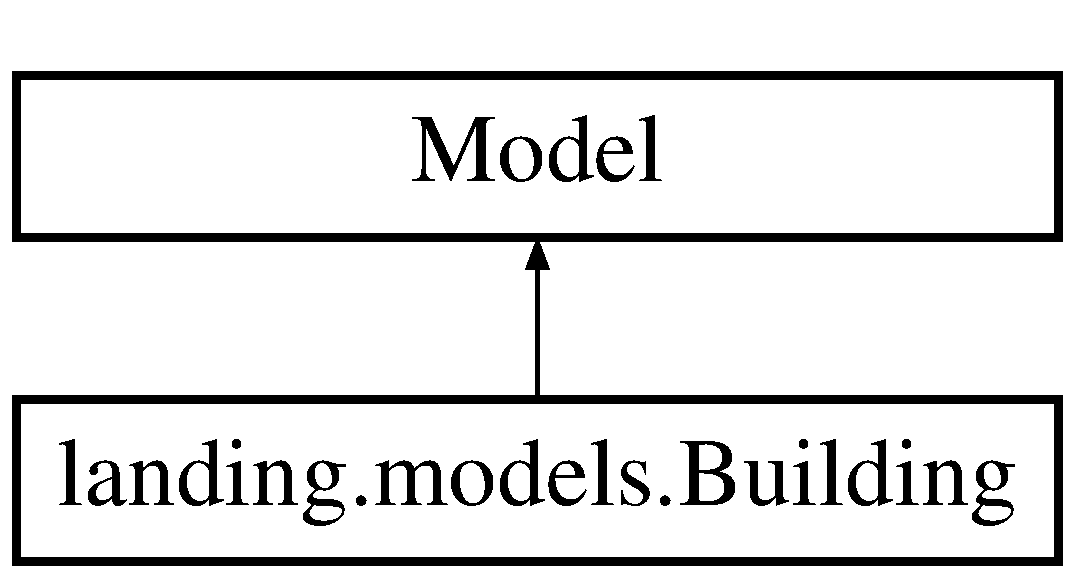
\includegraphics[height=2.000000cm]{classlanding_1_1models_1_1Building}
\end{center}
\end{figure}
\subsection*{Static Public Attributes}
\begin{DoxyCompactItemize}
\item 
\mbox{\hyperlink{classlanding_1_1models_1_1Building_abc0975a9fc05e581cdd3c386da7c0ab0}{building\+\_\+campus}} = models.\+Many\+To\+Many\+Field(\mbox{\hyperlink{classlanding_1_1models_1_1Campus}{Campus}})
\item 
\mbox{\hyperlink{classlanding_1_1models_1_1Building_aae60127da595f83f0284ebb34d566791}{building\+\_\+name}} = models.\+Char\+Field(max\+\_\+length=45)
\item 
\mbox{\hyperlink{classlanding_1_1models_1_1Building_a9a8dc99b835d9bf509d7eb35660ecfb0}{building\+\_\+room\+Number}} = models.\+Char\+Field(max\+\_\+length=8)
\end{DoxyCompactItemize}


\subsection{Detailed Description}
\begin{DoxyVerb}@Campus holds where classes are held, this includes the
        building name (i.e PKI), room number(i.e. 156), and campus(i.e. Scott (South) Campus.
        This allows for insights on the amount of time a student has to get to class.
\end{DoxyVerb}
 

Definition at line 104 of file models.\+py.



\subsection{Member Data Documentation}
\mbox{\Hypertarget{classlanding_1_1models_1_1Building_abc0975a9fc05e581cdd3c386da7c0ab0}\label{classlanding_1_1models_1_1Building_abc0975a9fc05e581cdd3c386da7c0ab0}} 
\index{landing\+::models\+::\+Building@{landing\+::models\+::\+Building}!building\+\_\+campus@{building\+\_\+campus}}
\index{building\+\_\+campus@{building\+\_\+campus}!landing\+::models\+::\+Building@{landing\+::models\+::\+Building}}
\subsubsection{\texorpdfstring{building\+\_\+campus}{building\_campus}}
{\footnotesize\ttfamily landing.\+models.\+Building.\+building\+\_\+campus = models.\+Many\+To\+Many\+Field(\mbox{\hyperlink{classlanding_1_1models_1_1Campus}{Campus}})\hspace{0.3cm}{\ttfamily [static]}}



Definition at line 112 of file models.\+py.

\mbox{\Hypertarget{classlanding_1_1models_1_1Building_aae60127da595f83f0284ebb34d566791}\label{classlanding_1_1models_1_1Building_aae60127da595f83f0284ebb34d566791}} 
\index{landing\+::models\+::\+Building@{landing\+::models\+::\+Building}!building\+\_\+name@{building\+\_\+name}}
\index{building\+\_\+name@{building\+\_\+name}!landing\+::models\+::\+Building@{landing\+::models\+::\+Building}}
\subsubsection{\texorpdfstring{building\+\_\+name}{building\_name}}
{\footnotesize\ttfamily landing.\+models.\+Building.\+building\+\_\+name = models.\+Char\+Field(max\+\_\+length=45)\hspace{0.3cm}{\ttfamily [static]}}



Definition at line 110 of file models.\+py.

\mbox{\Hypertarget{classlanding_1_1models_1_1Building_a9a8dc99b835d9bf509d7eb35660ecfb0}\label{classlanding_1_1models_1_1Building_a9a8dc99b835d9bf509d7eb35660ecfb0}} 
\index{landing\+::models\+::\+Building@{landing\+::models\+::\+Building}!building\+\_\+room\+Number@{building\+\_\+room\+Number}}
\index{building\+\_\+room\+Number@{building\+\_\+room\+Number}!landing\+::models\+::\+Building@{landing\+::models\+::\+Building}}
\subsubsection{\texorpdfstring{building\+\_\+room\+Number}{building\_roomNumber}}
{\footnotesize\ttfamily landing.\+models.\+Building.\+building\+\_\+room\+Number = models.\+Char\+Field(max\+\_\+length=8)\hspace{0.3cm}{\ttfamily [static]}}



Definition at line 111 of file models.\+py.



The documentation for this class was generated from the following file\+:\begin{DoxyCompactItemize}
\item 
mav\+Agenda/landing/\mbox{\hyperlink{models_8py}{models.\+py}}\end{DoxyCompactItemize}

\hypertarget{classlanding_1_1models_1_1Campus}{}\section{landing.\+models.\+Campus Class Reference}
\label{classlanding_1_1models_1_1Campus}\index{landing.\+models.\+Campus@{landing.\+models.\+Campus}}
Inheritance diagram for landing.\+models.\+Campus\+:\begin{figure}[H]
\begin{center}
\leavevmode
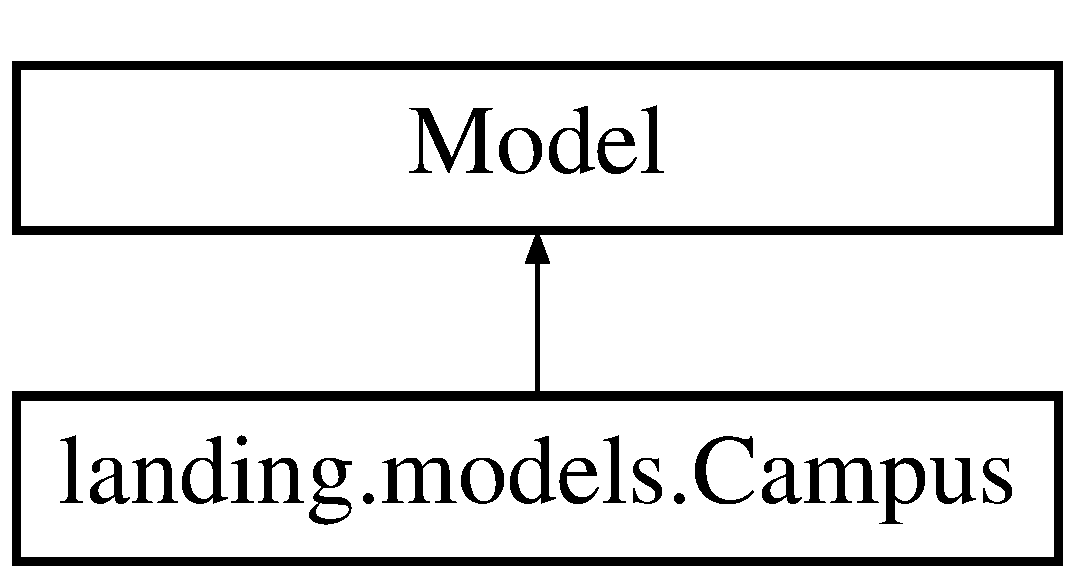
\includegraphics[height=2.000000cm]{classlanding_1_1models_1_1Campus}
\end{center}
\end{figure}
\subsection*{Static Public Attributes}
\begin{DoxyCompactItemize}
\item 
string \mbox{\hyperlink{classlanding_1_1models_1_1Campus_a399e7a0a49e00f3989ddcb279895289d}{B}} = \char`\"{}Center Street \mbox{\hyperlink{classlanding_1_1models_1_1Campus}{Campus}}\char`\"{}
\item 
\mbox{\hyperlink{classlanding_1_1models_1_1Campus_ae04580bc0816bb0de3b83563393375f6}{campus\+\_\+name}} = models.\+Char\+Field(max\+\_\+length=30, choices=\mbox{\hyperlink{classlanding_1_1models_1_1Campus_a7db95941da37de92bae99b10b9cdda5e}{S\+P\+E\+C\+I\+A\+L\+\_\+\+T\+Y\+P\+E\+\_\+\+C\+H\+O\+I\+CE}}, default=None)
\item 
string \mbox{\hyperlink{classlanding_1_1models_1_1Campus_a98b80c86220f75dbb0ece45713d02e09}{N}} = \char`\"{}North \mbox{\hyperlink{classlanding_1_1models_1_1Campus}{Campus}}\char`\"{}
\item 
string \mbox{\hyperlink{classlanding_1_1models_1_1Campus_ad81ec129890560554391f01ce266beaa}{S}} = \char`\"{}Scott (South) \mbox{\hyperlink{classlanding_1_1models_1_1Campus}{Campus}}\char`\"{}
\item 
tuple \mbox{\hyperlink{classlanding_1_1models_1_1Campus_a7db95941da37de92bae99b10b9cdda5e}{S\+P\+E\+C\+I\+A\+L\+\_\+\+T\+Y\+P\+E\+\_\+\+C\+H\+O\+I\+CE}}
\end{DoxyCompactItemize}


\subsection{Detailed Description}
\begin{DoxyVerb}@Campus holds where classes are held, this includes the
        campus name (i.e north campus). This allows for insights on
        the amount of time a student has to get to class.
\end{DoxyVerb}
 

Definition at line 88 of file models.\+py.



\subsection{Member Data Documentation}
\mbox{\Hypertarget{classlanding_1_1models_1_1Campus_a399e7a0a49e00f3989ddcb279895289d}\label{classlanding_1_1models_1_1Campus_a399e7a0a49e00f3989ddcb279895289d}} 
\index{landing\+::models\+::\+Campus@{landing\+::models\+::\+Campus}!B@{B}}
\index{B@{B}!landing\+::models\+::\+Campus@{landing\+::models\+::\+Campus}}
\subsubsection{\texorpdfstring{B}{B}}
{\footnotesize\ttfamily string landing.\+models.\+Campus.\+B = \char`\"{}Center Street \mbox{\hyperlink{classlanding_1_1models_1_1Campus}{Campus}}\char`\"{}\hspace{0.3cm}{\ttfamily [static]}}



Definition at line 96 of file models.\+py.

\mbox{\Hypertarget{classlanding_1_1models_1_1Campus_ae04580bc0816bb0de3b83563393375f6}\label{classlanding_1_1models_1_1Campus_ae04580bc0816bb0de3b83563393375f6}} 
\index{landing\+::models\+::\+Campus@{landing\+::models\+::\+Campus}!campus\+\_\+name@{campus\+\_\+name}}
\index{campus\+\_\+name@{campus\+\_\+name}!landing\+::models\+::\+Campus@{landing\+::models\+::\+Campus}}
\subsubsection{\texorpdfstring{campus\+\_\+name}{campus\_name}}
{\footnotesize\ttfamily landing.\+models.\+Campus.\+campus\+\_\+name = models.\+Char\+Field(max\+\_\+length=30, choices=\mbox{\hyperlink{classlanding_1_1models_1_1Campus_a7db95941da37de92bae99b10b9cdda5e}{S\+P\+E\+C\+I\+A\+L\+\_\+\+T\+Y\+P\+E\+\_\+\+C\+H\+O\+I\+CE}}, default=None)\hspace{0.3cm}{\ttfamily [static]}}



Definition at line 102 of file models.\+py.

\mbox{\Hypertarget{classlanding_1_1models_1_1Campus_a98b80c86220f75dbb0ece45713d02e09}\label{classlanding_1_1models_1_1Campus_a98b80c86220f75dbb0ece45713d02e09}} 
\index{landing\+::models\+::\+Campus@{landing\+::models\+::\+Campus}!N@{N}}
\index{N@{N}!landing\+::models\+::\+Campus@{landing\+::models\+::\+Campus}}
\subsubsection{\texorpdfstring{N}{N}}
{\footnotesize\ttfamily string landing.\+models.\+Campus.\+N = \char`\"{}North \mbox{\hyperlink{classlanding_1_1models_1_1Campus}{Campus}}\char`\"{}\hspace{0.3cm}{\ttfamily [static]}}



Definition at line 94 of file models.\+py.

\mbox{\Hypertarget{classlanding_1_1models_1_1Campus_ad81ec129890560554391f01ce266beaa}\label{classlanding_1_1models_1_1Campus_ad81ec129890560554391f01ce266beaa}} 
\index{landing\+::models\+::\+Campus@{landing\+::models\+::\+Campus}!S@{S}}
\index{S@{S}!landing\+::models\+::\+Campus@{landing\+::models\+::\+Campus}}
\subsubsection{\texorpdfstring{S}{S}}
{\footnotesize\ttfamily string landing.\+models.\+Campus.\+S = \char`\"{}Scott (South) \mbox{\hyperlink{classlanding_1_1models_1_1Campus}{Campus}}\char`\"{}\hspace{0.3cm}{\ttfamily [static]}}



Definition at line 95 of file models.\+py.

\mbox{\Hypertarget{classlanding_1_1models_1_1Campus_a7db95941da37de92bae99b10b9cdda5e}\label{classlanding_1_1models_1_1Campus_a7db95941da37de92bae99b10b9cdda5e}} 
\index{landing\+::models\+::\+Campus@{landing\+::models\+::\+Campus}!S\+P\+E\+C\+I\+A\+L\+\_\+\+T\+Y\+P\+E\+\_\+\+C\+H\+O\+I\+CE@{S\+P\+E\+C\+I\+A\+L\+\_\+\+T\+Y\+P\+E\+\_\+\+C\+H\+O\+I\+CE}}
\index{S\+P\+E\+C\+I\+A\+L\+\_\+\+T\+Y\+P\+E\+\_\+\+C\+H\+O\+I\+CE@{S\+P\+E\+C\+I\+A\+L\+\_\+\+T\+Y\+P\+E\+\_\+\+C\+H\+O\+I\+CE}!landing\+::models\+::\+Campus@{landing\+::models\+::\+Campus}}
\subsubsection{\texorpdfstring{S\+P\+E\+C\+I\+A\+L\+\_\+\+T\+Y\+P\+E\+\_\+\+C\+H\+O\+I\+CE}{SPECIAL\_TYPE\_CHOICE}}
{\footnotesize\ttfamily tuple landing.\+models.\+Campus.\+S\+P\+E\+C\+I\+A\+L\+\_\+\+T\+Y\+P\+E\+\_\+\+C\+H\+O\+I\+CE\hspace{0.3cm}{\ttfamily [static]}}

{\bfseries Initial value\+:}
\begin{DoxyCode}
=  (
        (N, \textcolor{stringliteral}{"North Campus"}),
        (S, \textcolor{stringliteral}{"Scott (South) Campus"}),
        (B, \textcolor{stringliteral}{"Center Street Campus"}),
    )
\end{DoxyCode}


Definition at line 97 of file models.\+py.



The documentation for this class was generated from the following file\+:\begin{DoxyCompactItemize}
\item 
mav\+Agenda/landing/\mbox{\hyperlink{models_8py}{models.\+py}}\end{DoxyCompactItemize}

\hypertarget{classlanding_1_1models_1_1Complete}{}\section{landing.\+models.\+Complete Class Reference}
\label{classlanding_1_1models_1_1Complete}\index{landing.\+models.\+Complete@{landing.\+models.\+Complete}}
Inheritance diagram for landing.\+models.\+Complete\+:\begin{figure}[H]
\begin{center}
\leavevmode
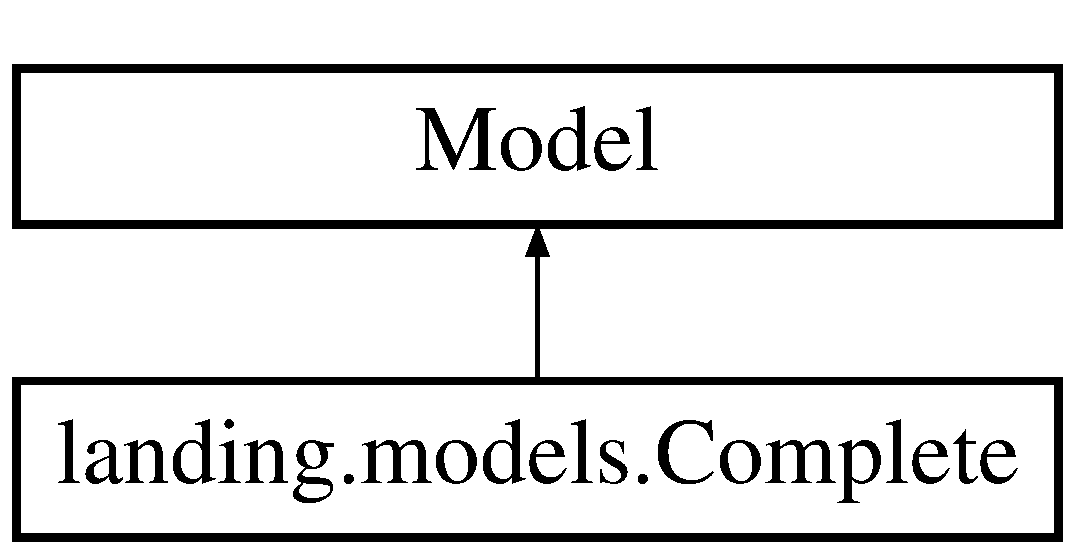
\includegraphics[height=2.000000cm]{classlanding_1_1models_1_1Complete}
\end{center}
\end{figure}
\subsection*{Static Public Attributes}
\begin{DoxyCompactItemize}
\item 
\mbox{\hyperlink{classlanding_1_1models_1_1Complete_a6573e7bb17c780113e804dc2978b937d}{complete\+\_\+courses}} = models.\+Many\+To\+Many\+Field(\mbox{\hyperlink{classlanding_1_1models_1_1Course}{Course}})
\item 
\mbox{\hyperlink{classlanding_1_1models_1_1Complete_a991355f0331ce0c2567ee5dd75c24897}{complete\+\_\+user}} = models.\+Foreign\+Key(User, on\+\_\+delete=models.\+C\+A\+S\+C\+A\+DE)
\end{DoxyCompactItemize}


\subsection{Detailed Description}
\begin{DoxyVerb}@Complete  holds classes that a specific user has completed,
        this includes the user and course tables to combine this information.
\end{DoxyVerb}
 

Definition at line 175 of file models.\+py.



\subsection{Member Data Documentation}
\mbox{\Hypertarget{classlanding_1_1models_1_1Complete_a6573e7bb17c780113e804dc2978b937d}\label{classlanding_1_1models_1_1Complete_a6573e7bb17c780113e804dc2978b937d}} 
\index{landing\+::models\+::\+Complete@{landing\+::models\+::\+Complete}!complete\+\_\+courses@{complete\+\_\+courses}}
\index{complete\+\_\+courses@{complete\+\_\+courses}!landing\+::models\+::\+Complete@{landing\+::models\+::\+Complete}}
\subsubsection{\texorpdfstring{complete\+\_\+courses}{complete\_courses}}
{\footnotesize\ttfamily landing.\+models.\+Complete.\+complete\+\_\+courses = models.\+Many\+To\+Many\+Field(\mbox{\hyperlink{classlanding_1_1models_1_1Course}{Course}})\hspace{0.3cm}{\ttfamily [static]}}



Definition at line 181 of file models.\+py.

\mbox{\Hypertarget{classlanding_1_1models_1_1Complete_a991355f0331ce0c2567ee5dd75c24897}\label{classlanding_1_1models_1_1Complete_a991355f0331ce0c2567ee5dd75c24897}} 
\index{landing\+::models\+::\+Complete@{landing\+::models\+::\+Complete}!complete\+\_\+user@{complete\+\_\+user}}
\index{complete\+\_\+user@{complete\+\_\+user}!landing\+::models\+::\+Complete@{landing\+::models\+::\+Complete}}
\subsubsection{\texorpdfstring{complete\+\_\+user}{complete\_user}}
{\footnotesize\ttfamily landing.\+models.\+Complete.\+complete\+\_\+user = models.\+Foreign\+Key(User, on\+\_\+delete=models.\+C\+A\+S\+C\+A\+DE)\hspace{0.3cm}{\ttfamily [static]}}



Definition at line 180 of file models.\+py.



The documentation for this class was generated from the following file\+:\begin{DoxyCompactItemize}
\item 
mav\+Agenda/landing/\mbox{\hyperlink{models_8py}{models.\+py}}\end{DoxyCompactItemize}

\hypertarget{classlanding_1_1models_1_1Course}{}\section{landing.\+models.\+Course Class Reference}
\label{classlanding_1_1models_1_1Course}\index{landing.\+models.\+Course@{landing.\+models.\+Course}}
Inheritance diagram for landing.\+models.\+Course\+:\begin{figure}[H]
\begin{center}
\leavevmode
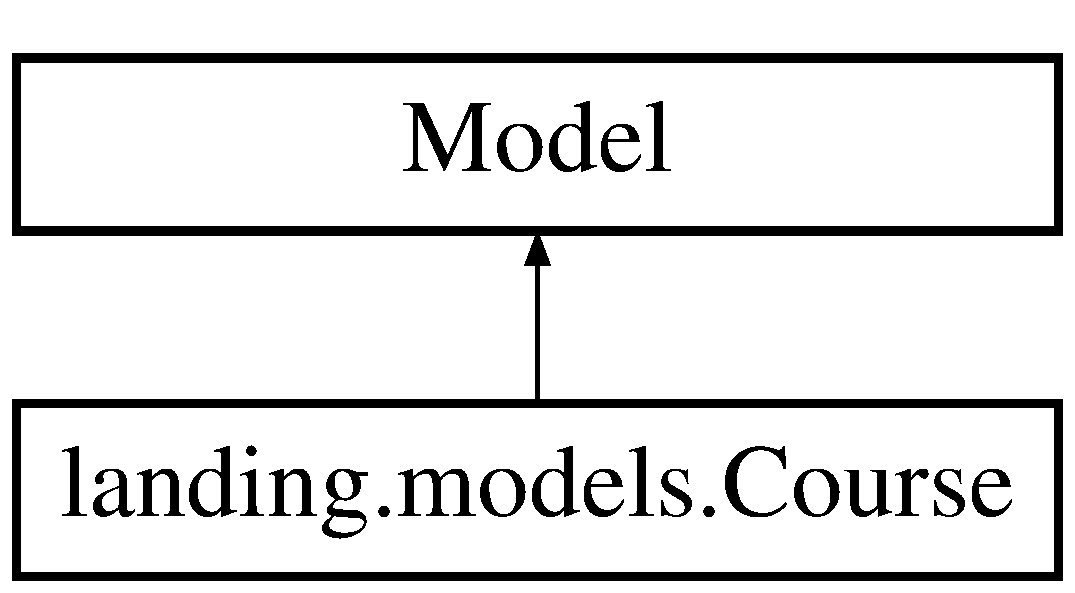
\includegraphics[height=2.000000cm]{classlanding_1_1models_1_1Course}
\end{center}
\end{figure}
\subsection*{Static Public Attributes}
\begin{DoxyCompactItemize}
\item 
string \mbox{\hyperlink{classlanding_1_1models_1_1Course_a9a6614f90db0d81754b98a123c43ecef}{A}} = \char`\"{}All\char`\"{}
\item 
\mbox{\hyperlink{classlanding_1_1models_1_1Course_abe19a335ae5a8e6e19bde096ef69b70d}{course\+\_\+comment}} = models.\+Char\+Field(max\+\_\+length=200, blank=True)
\item 
\mbox{\hyperlink{classlanding_1_1models_1_1Course_a2d5c8952932526241c8168ff624780fa}{course\+\_\+credits}} = models.\+Integer\+Field()
\item 
\mbox{\hyperlink{classlanding_1_1models_1_1Course_a6c3b552faf247213e88da70d3eab8551}{course\+\_\+name}} = models.\+Char\+Field(max\+\_\+length=75)
\item 
\mbox{\hyperlink{classlanding_1_1models_1_1Course_aa0134d6ca4ef236142fb0ac7670732a7}{course\+\_\+num}} = models.\+Char\+Field(max\+\_\+length=15)
\item 
\mbox{\hyperlink{classlanding_1_1models_1_1Course_a8d2a4c6f59aefe907d9d9cbd84a5ac5b}{course\+\_\+requirements}} = models.\+Foreign\+Key(\mbox{\hyperlink{classlanding_1_1models_1_1Requirement}{Requirement}}, on\+\_\+delete=models.\+C\+A\+S\+C\+A\+DE, null=True)
\item 
\mbox{\hyperlink{classlanding_1_1models_1_1Course_a1c139fd87a247369225dbe0388f72cce}{course\+\_\+semester}} = models.\+Char\+Field(max\+\_\+length=10, choices=\mbox{\hyperlink{classlanding_1_1models_1_1Course_af5c611e98c1a5fc7ee9c7f072af17631}{S\+E\+M\+\_\+\+C\+H\+O\+I\+CE}}, default=\mbox{\hyperlink{classlanding_1_1models_1_1Course_a9a6614f90db0d81754b98a123c43ecef}{A}})
\item 
\mbox{\hyperlink{classlanding_1_1models_1_1Course_a996761ee6b60fb089233e4f0878e96e4}{course\+\_\+special}} = models.\+Char\+Field(max\+\_\+length=15, choices=\mbox{\hyperlink{classlanding_1_1models_1_1Course_ac0a930e2ca556697d478cb97a894568b}{S\+P\+E\+C\+I\+A\+L\+\_\+\+T\+Y\+P\+E\+\_\+\+C\+H\+O\+I\+CE}}, default=None)
\item 
\mbox{\hyperlink{classlanding_1_1models_1_1Course_af4e65f18a31f13b3d33a5497b6d70a43}{course\+\_\+subject}} = models.\+Char\+Field(max\+\_\+length=15)
\item 
string \mbox{\hyperlink{classlanding_1_1models_1_1Course_aa11bad52172a59a7fa37ab291117abfd}{F}} = \char`\"{}Fall\char`\"{}
\item 
string \mbox{\hyperlink{classlanding_1_1models_1_1Course_ae7b25314cb92ae2a3028d7b040f16ed5}{M}} = \char`\"{}Summer\char`\"{}
\item 
string \mbox{\hyperlink{classlanding_1_1models_1_1Course_a228c31655e120c1bf499f848c70534e9}{N}} = \char`\"{}No\char`\"{}
\item 
string \mbox{\hyperlink{classlanding_1_1models_1_1Course_a91e4bb24a46ec40f82d0d1c8bb1f5705}{S}} = \char`\"{}Spring\char`\"{}
\item 
tuple \mbox{\hyperlink{classlanding_1_1models_1_1Course_af5c611e98c1a5fc7ee9c7f072af17631}{S\+E\+M\+\_\+\+C\+H\+O\+I\+CE}}
\item 
tuple \mbox{\hyperlink{classlanding_1_1models_1_1Course_ac0a930e2ca556697d478cb97a894568b}{S\+P\+E\+C\+I\+A\+L\+\_\+\+T\+Y\+P\+E\+\_\+\+C\+H\+O\+I\+CE}}
\item 
string \mbox{\hyperlink{classlanding_1_1models_1_1Course_af5424af7cbb7df0adff059a54ddbf933}{W}} = \char`\"{}Waiver\char`\"{}
\item 
string \mbox{\hyperlink{classlanding_1_1models_1_1Course_a00ccedd8d49ed021b01bbe1aea40ebe3}{Y}} = \char`\"{}Lab\char`\"{}
\end{DoxyCompactItemize}


\subsection{Detailed Description}
\begin{DoxyVerb}@Course holds the systems classes, this includes the
        name (i.e Java 1), subject (i.e. IS&T), semester it is offered in (i.e. Spring and Fall),
        special flag if it has an extra requirement (i.e. lab), comment for any other special
        characteristics (i.e. capstone must be taken in the last semester),
        credits (i.e. 3), and num (1400).
\end{DoxyVerb}
 

Definition at line 53 of file models.\+py.



\subsection{Member Data Documentation}
\mbox{\Hypertarget{classlanding_1_1models_1_1Course_a9a6614f90db0d81754b98a123c43ecef}\label{classlanding_1_1models_1_1Course_a9a6614f90db0d81754b98a123c43ecef}} 
\index{landing\+::models\+::\+Course@{landing\+::models\+::\+Course}!A@{A}}
\index{A@{A}!landing\+::models\+::\+Course@{landing\+::models\+::\+Course}}
\subsubsection{\texorpdfstring{A}{A}}
{\footnotesize\ttfamily string landing.\+models.\+Course.\+A = \char`\"{}All\char`\"{}\hspace{0.3cm}{\ttfamily [static]}}



Definition at line 64 of file models.\+py.

\mbox{\Hypertarget{classlanding_1_1models_1_1Course_abe19a335ae5a8e6e19bde096ef69b70d}\label{classlanding_1_1models_1_1Course_abe19a335ae5a8e6e19bde096ef69b70d}} 
\index{landing\+::models\+::\+Course@{landing\+::models\+::\+Course}!course\+\_\+comment@{course\+\_\+comment}}
\index{course\+\_\+comment@{course\+\_\+comment}!landing\+::models\+::\+Course@{landing\+::models\+::\+Course}}
\subsubsection{\texorpdfstring{course\+\_\+comment}{course\_comment}}
{\footnotesize\ttfamily landing.\+models.\+Course.\+course\+\_\+comment = models.\+Char\+Field(max\+\_\+length=200, blank=True)\hspace{0.3cm}{\ttfamily [static]}}



Definition at line 85 of file models.\+py.

\mbox{\Hypertarget{classlanding_1_1models_1_1Course_a2d5c8952932526241c8168ff624780fa}\label{classlanding_1_1models_1_1Course_a2d5c8952932526241c8168ff624780fa}} 
\index{landing\+::models\+::\+Course@{landing\+::models\+::\+Course}!course\+\_\+credits@{course\+\_\+credits}}
\index{course\+\_\+credits@{course\+\_\+credits}!landing\+::models\+::\+Course@{landing\+::models\+::\+Course}}
\subsubsection{\texorpdfstring{course\+\_\+credits}{course\_credits}}
{\footnotesize\ttfamily landing.\+models.\+Course.\+course\+\_\+credits = models.\+Integer\+Field()\hspace{0.3cm}{\ttfamily [static]}}



Definition at line 75 of file models.\+py.

\mbox{\Hypertarget{classlanding_1_1models_1_1Course_a6c3b552faf247213e88da70d3eab8551}\label{classlanding_1_1models_1_1Course_a6c3b552faf247213e88da70d3eab8551}} 
\index{landing\+::models\+::\+Course@{landing\+::models\+::\+Course}!course\+\_\+name@{course\+\_\+name}}
\index{course\+\_\+name@{course\+\_\+name}!landing\+::models\+::\+Course@{landing\+::models\+::\+Course}}
\subsubsection{\texorpdfstring{course\+\_\+name}{course\_name}}
{\footnotesize\ttfamily landing.\+models.\+Course.\+course\+\_\+name = models.\+Char\+Field(max\+\_\+length=75)\hspace{0.3cm}{\ttfamily [static]}}



Definition at line 61 of file models.\+py.

\mbox{\Hypertarget{classlanding_1_1models_1_1Course_aa0134d6ca4ef236142fb0ac7670732a7}\label{classlanding_1_1models_1_1Course_aa0134d6ca4ef236142fb0ac7670732a7}} 
\index{landing\+::models\+::\+Course@{landing\+::models\+::\+Course}!course\+\_\+num@{course\+\_\+num}}
\index{course\+\_\+num@{course\+\_\+num}!landing\+::models\+::\+Course@{landing\+::models\+::\+Course}}
\subsubsection{\texorpdfstring{course\+\_\+num}{course\_num}}
{\footnotesize\ttfamily landing.\+models.\+Course.\+course\+\_\+num = models.\+Char\+Field(max\+\_\+length=15)\hspace{0.3cm}{\ttfamily [static]}}



Definition at line 63 of file models.\+py.

\mbox{\Hypertarget{classlanding_1_1models_1_1Course_a8d2a4c6f59aefe907d9d9cbd84a5ac5b}\label{classlanding_1_1models_1_1Course_a8d2a4c6f59aefe907d9d9cbd84a5ac5b}} 
\index{landing\+::models\+::\+Course@{landing\+::models\+::\+Course}!course\+\_\+requirements@{course\+\_\+requirements}}
\index{course\+\_\+requirements@{course\+\_\+requirements}!landing\+::models\+::\+Course@{landing\+::models\+::\+Course}}
\subsubsection{\texorpdfstring{course\+\_\+requirements}{course\_requirements}}
{\footnotesize\ttfamily landing.\+models.\+Course.\+course\+\_\+requirements = models.\+Foreign\+Key(\mbox{\hyperlink{classlanding_1_1models_1_1Requirement}{Requirement}}, on\+\_\+delete=models.\+C\+A\+S\+C\+A\+DE, null=True)\hspace{0.3cm}{\ttfamily [static]}}



Definition at line 86 of file models.\+py.

\mbox{\Hypertarget{classlanding_1_1models_1_1Course_a1c139fd87a247369225dbe0388f72cce}\label{classlanding_1_1models_1_1Course_a1c139fd87a247369225dbe0388f72cce}} 
\index{landing\+::models\+::\+Course@{landing\+::models\+::\+Course}!course\+\_\+semester@{course\+\_\+semester}}
\index{course\+\_\+semester@{course\+\_\+semester}!landing\+::models\+::\+Course@{landing\+::models\+::\+Course}}
\subsubsection{\texorpdfstring{course\+\_\+semester}{course\_semester}}
{\footnotesize\ttfamily landing.\+models.\+Course.\+course\+\_\+semester = models.\+Char\+Field(max\+\_\+length=10, choices=\mbox{\hyperlink{classlanding_1_1models_1_1Course_af5c611e98c1a5fc7ee9c7f072af17631}{S\+E\+M\+\_\+\+C\+H\+O\+I\+CE}}, default=\mbox{\hyperlink{classlanding_1_1models_1_1Course_a9a6614f90db0d81754b98a123c43ecef}{A}})\hspace{0.3cm}{\ttfamily [static]}}



Definition at line 74 of file models.\+py.

\mbox{\Hypertarget{classlanding_1_1models_1_1Course_a996761ee6b60fb089233e4f0878e96e4}\label{classlanding_1_1models_1_1Course_a996761ee6b60fb089233e4f0878e96e4}} 
\index{landing\+::models\+::\+Course@{landing\+::models\+::\+Course}!course\+\_\+special@{course\+\_\+special}}
\index{course\+\_\+special@{course\+\_\+special}!landing\+::models\+::\+Course@{landing\+::models\+::\+Course}}
\subsubsection{\texorpdfstring{course\+\_\+special}{course\_special}}
{\footnotesize\ttfamily landing.\+models.\+Course.\+course\+\_\+special = models.\+Char\+Field(max\+\_\+length=15, choices=\mbox{\hyperlink{classlanding_1_1models_1_1Course_ac0a930e2ca556697d478cb97a894568b}{S\+P\+E\+C\+I\+A\+L\+\_\+\+T\+Y\+P\+E\+\_\+\+C\+H\+O\+I\+CE}}, default=None)\hspace{0.3cm}{\ttfamily [static]}}



Definition at line 84 of file models.\+py.

\mbox{\Hypertarget{classlanding_1_1models_1_1Course_af4e65f18a31f13b3d33a5497b6d70a43}\label{classlanding_1_1models_1_1Course_af4e65f18a31f13b3d33a5497b6d70a43}} 
\index{landing\+::models\+::\+Course@{landing\+::models\+::\+Course}!course\+\_\+subject@{course\+\_\+subject}}
\index{course\+\_\+subject@{course\+\_\+subject}!landing\+::models\+::\+Course@{landing\+::models\+::\+Course}}
\subsubsection{\texorpdfstring{course\+\_\+subject}{course\_subject}}
{\footnotesize\ttfamily landing.\+models.\+Course.\+course\+\_\+subject = models.\+Char\+Field(max\+\_\+length=15)\hspace{0.3cm}{\ttfamily [static]}}



Definition at line 62 of file models.\+py.

\mbox{\Hypertarget{classlanding_1_1models_1_1Course_aa11bad52172a59a7fa37ab291117abfd}\label{classlanding_1_1models_1_1Course_aa11bad52172a59a7fa37ab291117abfd}} 
\index{landing\+::models\+::\+Course@{landing\+::models\+::\+Course}!F@{F}}
\index{F@{F}!landing\+::models\+::\+Course@{landing\+::models\+::\+Course}}
\subsubsection{\texorpdfstring{F}{F}}
{\footnotesize\ttfamily string landing.\+models.\+Course.\+F = \char`\"{}Fall\char`\"{}\hspace{0.3cm}{\ttfamily [static]}}



Definition at line 66 of file models.\+py.

\mbox{\Hypertarget{classlanding_1_1models_1_1Course_ae7b25314cb92ae2a3028d7b040f16ed5}\label{classlanding_1_1models_1_1Course_ae7b25314cb92ae2a3028d7b040f16ed5}} 
\index{landing\+::models\+::\+Course@{landing\+::models\+::\+Course}!M@{M}}
\index{M@{M}!landing\+::models\+::\+Course@{landing\+::models\+::\+Course}}
\subsubsection{\texorpdfstring{M}{M}}
{\footnotesize\ttfamily string landing.\+models.\+Course.\+M = \char`\"{}Summer\char`\"{}\hspace{0.3cm}{\ttfamily [static]}}



Definition at line 67 of file models.\+py.

\mbox{\Hypertarget{classlanding_1_1models_1_1Course_a228c31655e120c1bf499f848c70534e9}\label{classlanding_1_1models_1_1Course_a228c31655e120c1bf499f848c70534e9}} 
\index{landing\+::models\+::\+Course@{landing\+::models\+::\+Course}!N@{N}}
\index{N@{N}!landing\+::models\+::\+Course@{landing\+::models\+::\+Course}}
\subsubsection{\texorpdfstring{N}{N}}
{\footnotesize\ttfamily string landing.\+models.\+Course.\+N = \char`\"{}No\char`\"{}\hspace{0.3cm}{\ttfamily [static]}}



Definition at line 76 of file models.\+py.

\mbox{\Hypertarget{classlanding_1_1models_1_1Course_a91e4bb24a46ec40f82d0d1c8bb1f5705}\label{classlanding_1_1models_1_1Course_a91e4bb24a46ec40f82d0d1c8bb1f5705}} 
\index{landing\+::models\+::\+Course@{landing\+::models\+::\+Course}!S@{S}}
\index{S@{S}!landing\+::models\+::\+Course@{landing\+::models\+::\+Course}}
\subsubsection{\texorpdfstring{S}{S}}
{\footnotesize\ttfamily string landing.\+models.\+Course.\+S = \char`\"{}Spring\char`\"{}\hspace{0.3cm}{\ttfamily [static]}}



Definition at line 65 of file models.\+py.

\mbox{\Hypertarget{classlanding_1_1models_1_1Course_af5c611e98c1a5fc7ee9c7f072af17631}\label{classlanding_1_1models_1_1Course_af5c611e98c1a5fc7ee9c7f072af17631}} 
\index{landing\+::models\+::\+Course@{landing\+::models\+::\+Course}!S\+E\+M\+\_\+\+C\+H\+O\+I\+CE@{S\+E\+M\+\_\+\+C\+H\+O\+I\+CE}}
\index{S\+E\+M\+\_\+\+C\+H\+O\+I\+CE@{S\+E\+M\+\_\+\+C\+H\+O\+I\+CE}!landing\+::models\+::\+Course@{landing\+::models\+::\+Course}}
\subsubsection{\texorpdfstring{S\+E\+M\+\_\+\+C\+H\+O\+I\+CE}{SEM\_CHOICE}}
{\footnotesize\ttfamily tuple landing.\+models.\+Course.\+S\+E\+M\+\_\+\+C\+H\+O\+I\+CE\hspace{0.3cm}{\ttfamily [static]}}

{\bfseries Initial value\+:}
\begin{DoxyCode}
=  (
        (A, \textcolor{stringliteral}{"All"}),
        (S, \textcolor{stringliteral}{"Spring"}),
        (F, \textcolor{stringliteral}{"Fall"}),
        (M, \textcolor{stringliteral}{"Summer"}),
    )
\end{DoxyCode}


Definition at line 68 of file models.\+py.

\mbox{\Hypertarget{classlanding_1_1models_1_1Course_ac0a930e2ca556697d478cb97a894568b}\label{classlanding_1_1models_1_1Course_ac0a930e2ca556697d478cb97a894568b}} 
\index{landing\+::models\+::\+Course@{landing\+::models\+::\+Course}!S\+P\+E\+C\+I\+A\+L\+\_\+\+T\+Y\+P\+E\+\_\+\+C\+H\+O\+I\+CE@{S\+P\+E\+C\+I\+A\+L\+\_\+\+T\+Y\+P\+E\+\_\+\+C\+H\+O\+I\+CE}}
\index{S\+P\+E\+C\+I\+A\+L\+\_\+\+T\+Y\+P\+E\+\_\+\+C\+H\+O\+I\+CE@{S\+P\+E\+C\+I\+A\+L\+\_\+\+T\+Y\+P\+E\+\_\+\+C\+H\+O\+I\+CE}!landing\+::models\+::\+Course@{landing\+::models\+::\+Course}}
\subsubsection{\texorpdfstring{S\+P\+E\+C\+I\+A\+L\+\_\+\+T\+Y\+P\+E\+\_\+\+C\+H\+O\+I\+CE}{SPECIAL\_TYPE\_CHOICE}}
{\footnotesize\ttfamily tuple landing.\+models.\+Course.\+S\+P\+E\+C\+I\+A\+L\+\_\+\+T\+Y\+P\+E\+\_\+\+C\+H\+O\+I\+CE\hspace{0.3cm}{\ttfamily [static]}}

{\bfseries Initial value\+:}
\begin{DoxyCode}
=  (
        (N, \textcolor{stringliteral}{"No"}),
        (Y, \textcolor{stringliteral}{"Lab"}),
        (W, \textcolor{stringliteral}{"Waiver"}),
    )
\end{DoxyCode}


Definition at line 79 of file models.\+py.

\mbox{\Hypertarget{classlanding_1_1models_1_1Course_af5424af7cbb7df0adff059a54ddbf933}\label{classlanding_1_1models_1_1Course_af5424af7cbb7df0adff059a54ddbf933}} 
\index{landing\+::models\+::\+Course@{landing\+::models\+::\+Course}!W@{W}}
\index{W@{W}!landing\+::models\+::\+Course@{landing\+::models\+::\+Course}}
\subsubsection{\texorpdfstring{W}{W}}
{\footnotesize\ttfamily string landing.\+models.\+Course.\+W = \char`\"{}Waiver\char`\"{}\hspace{0.3cm}{\ttfamily [static]}}



Definition at line 78 of file models.\+py.

\mbox{\Hypertarget{classlanding_1_1models_1_1Course_a00ccedd8d49ed021b01bbe1aea40ebe3}\label{classlanding_1_1models_1_1Course_a00ccedd8d49ed021b01bbe1aea40ebe3}} 
\index{landing\+::models\+::\+Course@{landing\+::models\+::\+Course}!Y@{Y}}
\index{Y@{Y}!landing\+::models\+::\+Course@{landing\+::models\+::\+Course}}
\subsubsection{\texorpdfstring{Y}{Y}}
{\footnotesize\ttfamily string landing.\+models.\+Course.\+Y = \char`\"{}Lab\char`\"{}\hspace{0.3cm}{\ttfamily [static]}}



Definition at line 77 of file models.\+py.



The documentation for this class was generated from the following file\+:\begin{DoxyCompactItemize}
\item 
mav\+Agenda/landing/\mbox{\hyperlink{models_8py}{models.\+py}}\end{DoxyCompactItemize}

\hypertarget{classlanding_1_1models_1_1Degree}{}\section{landing.\+models.\+Degree Class Reference}
\label{classlanding_1_1models_1_1Degree}\index{landing.\+models.\+Degree@{landing.\+models.\+Degree}}
Inheritance diagram for landing.\+models.\+Degree\+:\begin{figure}[H]
\begin{center}
\leavevmode
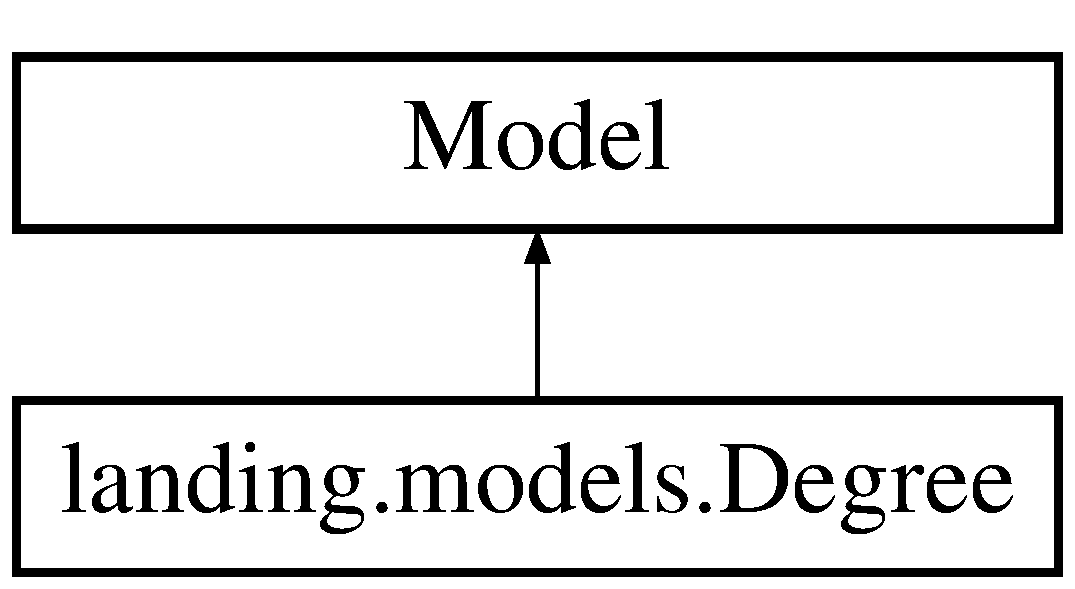
\includegraphics[height=2.000000cm]{classlanding_1_1models_1_1Degree}
\end{center}
\end{figure}
\subsection*{Static Public Attributes}
\begin{DoxyCompactItemize}
\item 
string \mbox{\hyperlink{classlanding_1_1models_1_1Degree_afc3f658c11fb395b63ec02dea12d73ff}{B\+I\+OI}} = \textquotesingle{}Bioinformatics\textquotesingle{}
\item 
string \mbox{\hyperlink{classlanding_1_1models_1_1Degree_a22b6e40d619611a02ecd1750b0cfcd22}{BS}} = \textquotesingle{}Bachelor of Science\textquotesingle{}
\item 
string \mbox{\hyperlink{classlanding_1_1models_1_1Degree_a648e73a8b3abcfe249775ca0e0902a46}{C\+ON}} = \textquotesingle{}Concentration\textquotesingle{}
\item 
string \mbox{\hyperlink{classlanding_1_1models_1_1Degree_a818c1f18f64c3529a2bfcb746efb6600}{C\+S\+CI}} = \textquotesingle{}Computer Science\textquotesingle{}
\item 
string \mbox{\hyperlink{classlanding_1_1models_1_1Degree_a6ce9e89d5029462e65272bc7b145d4dd}{C\+Y\+BR}} = \textquotesingle{}Cybersecurity\textquotesingle{}
\item 
\mbox{\hyperlink{classlanding_1_1models_1_1Degree_abe092b826ebd50d242cf880ca10e127b}{degree\+\_\+diploma}} = models.\+Char\+Field(max\+\_\+length=50, choices=\mbox{\hyperlink{classlanding_1_1models_1_1Degree_a7972b49cb5153c95f5a5d509de3b1135}{D\+I\+P\+L\+O\+M\+A\+\_\+\+C\+H\+O\+I\+CE}}, default=\mbox{\hyperlink{classlanding_1_1models_1_1Degree_a22b6e40d619611a02ecd1750b0cfcd22}{BS}})
\item 
\mbox{\hyperlink{classlanding_1_1models_1_1Degree_a5dbec6bcca9df5d74244218ef8e75a5b}{degree\+\_\+track}} = models.\+Char\+Field(max\+\_\+length=50, choices=\mbox{\hyperlink{classlanding_1_1models_1_1Degree_a63995a5c2aa1f03f1328238ebbd7ecd2}{T\+R\+A\+C\+K\+\_\+\+C\+H\+O\+I\+CE}}, default=\mbox{\hyperlink{classlanding_1_1models_1_1Degree_a818c1f18f64c3529a2bfcb746efb6600}{C\+S\+CI}})
\item 
\mbox{\hyperlink{classlanding_1_1models_1_1Degree_a15ee92cd794ad8c2dabf965723cfd949}{degree\+\_\+type}} = models.\+Char\+Field(max\+\_\+length=50, choices=\mbox{\hyperlink{classlanding_1_1models_1_1Degree_a2e0c65757b0f59ed5c62ee8b2d517300}{T\+Y\+P\+E\+\_\+\+C\+H\+O\+I\+CE}}, default=\mbox{\hyperlink{classlanding_1_1models_1_1Degree_ad19df1851aacc963e0bc67c2a7097aec}{M\+AJ}})
\item 
\mbox{\hyperlink{classlanding_1_1models_1_1Degree_ab548201fcb3ef2b2455ba7311fdfcb26}{degree\+\_\+users}} = models.\+Many\+To\+Many\+Field(User)
\item 
tuple \mbox{\hyperlink{classlanding_1_1models_1_1Degree_a7972b49cb5153c95f5a5d509de3b1135}{D\+I\+P\+L\+O\+M\+A\+\_\+\+C\+H\+O\+I\+CE}}
\item 
string \mbox{\hyperlink{classlanding_1_1models_1_1Degree_a0d92d2c83362111ad3cf7ee19d107897}{I\+T\+IN}} = \textquotesingle{}IT Innovation\textquotesingle{}
\item 
string \mbox{\hyperlink{classlanding_1_1models_1_1Degree_ad19df1851aacc963e0bc67c2a7097aec}{M\+AJ}} = \textquotesingle{}Major\textquotesingle{}
\item 
string \mbox{\hyperlink{classlanding_1_1models_1_1Degree_af38536acc307300df46363d93eb48b24}{M\+IN}} = \textquotesingle{}Minor\textquotesingle{}
\item 
string \mbox{\hyperlink{classlanding_1_1models_1_1Degree_a88793e29b02916081124dfba858b598e}{M\+IS}} = \textquotesingle{}Management Information Systems\textquotesingle{}
\item 
string \mbox{\hyperlink{classlanding_1_1models_1_1Degree_ae9b848406afe10cc7edb6dfcc4a78d1d}{MS}} = \textquotesingle{}Master of Science\textquotesingle{}
\item 
string \mbox{\hyperlink{classlanding_1_1models_1_1Degree_a324175b93dbc6add6feb3e954b2a7b6b}{Ph\+DS}} = \textquotesingle{}Doctor of Science\textquotesingle{}
\item 
tuple \mbox{\hyperlink{classlanding_1_1models_1_1Degree_a63995a5c2aa1f03f1328238ebbd7ecd2}{T\+R\+A\+C\+K\+\_\+\+C\+H\+O\+I\+CE}}
\item 
tuple \mbox{\hyperlink{classlanding_1_1models_1_1Degree_a2e0c65757b0f59ed5c62ee8b2d517300}{T\+Y\+P\+E\+\_\+\+C\+H\+O\+I\+CE}}
\end{DoxyCompactItemize}


\subsection{Detailed Description}
\begin{DoxyVerb}@Degree holds the degree a user would have, this includes the
        diploma (i.e Bachelor of Science), type (i.e. major),
        and track (i.e. computer science).
\end{DoxyVerb}
 

Definition at line 4 of file models.\+py.



\subsection{Member Data Documentation}
\mbox{\Hypertarget{classlanding_1_1models_1_1Degree_afc3f658c11fb395b63ec02dea12d73ff}\label{classlanding_1_1models_1_1Degree_afc3f658c11fb395b63ec02dea12d73ff}} 
\index{landing\+::models\+::\+Degree@{landing\+::models\+::\+Degree}!B\+I\+OI@{B\+I\+OI}}
\index{B\+I\+OI@{B\+I\+OI}!landing\+::models\+::\+Degree@{landing\+::models\+::\+Degree}}
\subsubsection{\texorpdfstring{B\+I\+OI}{BIOI}}
{\footnotesize\ttfamily string landing.\+models.\+Degree.\+B\+I\+OI = \textquotesingle{}Bioinformatics\textquotesingle{}\hspace{0.3cm}{\ttfamily [static]}}



Definition at line 30 of file models.\+py.

\mbox{\Hypertarget{classlanding_1_1models_1_1Degree_a22b6e40d619611a02ecd1750b0cfcd22}\label{classlanding_1_1models_1_1Degree_a22b6e40d619611a02ecd1750b0cfcd22}} 
\index{landing\+::models\+::\+Degree@{landing\+::models\+::\+Degree}!BS@{BS}}
\index{BS@{BS}!landing\+::models\+::\+Degree@{landing\+::models\+::\+Degree}}
\subsubsection{\texorpdfstring{BS}{BS}}
{\footnotesize\ttfamily string landing.\+models.\+Degree.\+BS = \textquotesingle{}Bachelor of Science\textquotesingle{}\hspace{0.3cm}{\ttfamily [static]}}



Definition at line 10 of file models.\+py.

\mbox{\Hypertarget{classlanding_1_1models_1_1Degree_a648e73a8b3abcfe249775ca0e0902a46}\label{classlanding_1_1models_1_1Degree_a648e73a8b3abcfe249775ca0e0902a46}} 
\index{landing\+::models\+::\+Degree@{landing\+::models\+::\+Degree}!C\+ON@{C\+ON}}
\index{C\+ON@{C\+ON}!landing\+::models\+::\+Degree@{landing\+::models\+::\+Degree}}
\subsubsection{\texorpdfstring{C\+ON}{CON}}
{\footnotesize\ttfamily string landing.\+models.\+Degree.\+C\+ON = \textquotesingle{}Concentration\textquotesingle{}\hspace{0.3cm}{\ttfamily [static]}}



Definition at line 21 of file models.\+py.

\mbox{\Hypertarget{classlanding_1_1models_1_1Degree_a818c1f18f64c3529a2bfcb746efb6600}\label{classlanding_1_1models_1_1Degree_a818c1f18f64c3529a2bfcb746efb6600}} 
\index{landing\+::models\+::\+Degree@{landing\+::models\+::\+Degree}!C\+S\+CI@{C\+S\+CI}}
\index{C\+S\+CI@{C\+S\+CI}!landing\+::models\+::\+Degree@{landing\+::models\+::\+Degree}}
\subsubsection{\texorpdfstring{C\+S\+CI}{CSCI}}
{\footnotesize\ttfamily string landing.\+models.\+Degree.\+C\+S\+CI = \textquotesingle{}Computer Science\textquotesingle{}\hspace{0.3cm}{\ttfamily [static]}}



Definition at line 28 of file models.\+py.

\mbox{\Hypertarget{classlanding_1_1models_1_1Degree_a6ce9e89d5029462e65272bc7b145d4dd}\label{classlanding_1_1models_1_1Degree_a6ce9e89d5029462e65272bc7b145d4dd}} 
\index{landing\+::models\+::\+Degree@{landing\+::models\+::\+Degree}!C\+Y\+BR@{C\+Y\+BR}}
\index{C\+Y\+BR@{C\+Y\+BR}!landing\+::models\+::\+Degree@{landing\+::models\+::\+Degree}}
\subsubsection{\texorpdfstring{C\+Y\+BR}{CYBR}}
{\footnotesize\ttfamily string landing.\+models.\+Degree.\+C\+Y\+BR = \textquotesingle{}Cybersecurity\textquotesingle{}\hspace{0.3cm}{\ttfamily [static]}}



Definition at line 32 of file models.\+py.

\mbox{\Hypertarget{classlanding_1_1models_1_1Degree_abe092b826ebd50d242cf880ca10e127b}\label{classlanding_1_1models_1_1Degree_abe092b826ebd50d242cf880ca10e127b}} 
\index{landing\+::models\+::\+Degree@{landing\+::models\+::\+Degree}!degree\+\_\+diploma@{degree\+\_\+diploma}}
\index{degree\+\_\+diploma@{degree\+\_\+diploma}!landing\+::models\+::\+Degree@{landing\+::models\+::\+Degree}}
\subsubsection{\texorpdfstring{degree\+\_\+diploma}{degree\_diploma}}
{\footnotesize\ttfamily landing.\+models.\+Degree.\+degree\+\_\+diploma = models.\+Char\+Field(max\+\_\+length=50, choices=\mbox{\hyperlink{classlanding_1_1models_1_1Degree_a7972b49cb5153c95f5a5d509de3b1135}{D\+I\+P\+L\+O\+M\+A\+\_\+\+C\+H\+O\+I\+CE}}, default=\mbox{\hyperlink{classlanding_1_1models_1_1Degree_a22b6e40d619611a02ecd1750b0cfcd22}{BS}})\hspace{0.3cm}{\ttfamily [static]}}



Definition at line 18 of file models.\+py.

\mbox{\Hypertarget{classlanding_1_1models_1_1Degree_a5dbec6bcca9df5d74244218ef8e75a5b}\label{classlanding_1_1models_1_1Degree_a5dbec6bcca9df5d74244218ef8e75a5b}} 
\index{landing\+::models\+::\+Degree@{landing\+::models\+::\+Degree}!degree\+\_\+track@{degree\+\_\+track}}
\index{degree\+\_\+track@{degree\+\_\+track}!landing\+::models\+::\+Degree@{landing\+::models\+::\+Degree}}
\subsubsection{\texorpdfstring{degree\+\_\+track}{degree\_track}}
{\footnotesize\ttfamily landing.\+models.\+Degree.\+degree\+\_\+track = models.\+Char\+Field(max\+\_\+length=50, choices=\mbox{\hyperlink{classlanding_1_1models_1_1Degree_a63995a5c2aa1f03f1328238ebbd7ecd2}{T\+R\+A\+C\+K\+\_\+\+C\+H\+O\+I\+CE}}, default=\mbox{\hyperlink{classlanding_1_1models_1_1Degree_a818c1f18f64c3529a2bfcb746efb6600}{C\+S\+CI}})\hspace{0.3cm}{\ttfamily [static]}}



Definition at line 40 of file models.\+py.

\mbox{\Hypertarget{classlanding_1_1models_1_1Degree_a15ee92cd794ad8c2dabf965723cfd949}\label{classlanding_1_1models_1_1Degree_a15ee92cd794ad8c2dabf965723cfd949}} 
\index{landing\+::models\+::\+Degree@{landing\+::models\+::\+Degree}!degree\+\_\+type@{degree\+\_\+type}}
\index{degree\+\_\+type@{degree\+\_\+type}!landing\+::models\+::\+Degree@{landing\+::models\+::\+Degree}}
\subsubsection{\texorpdfstring{degree\+\_\+type}{degree\_type}}
{\footnotesize\ttfamily landing.\+models.\+Degree.\+degree\+\_\+type = models.\+Char\+Field(max\+\_\+length=50, choices=\mbox{\hyperlink{classlanding_1_1models_1_1Degree_a2e0c65757b0f59ed5c62ee8b2d517300}{T\+Y\+P\+E\+\_\+\+C\+H\+O\+I\+CE}}, default=\mbox{\hyperlink{classlanding_1_1models_1_1Degree_ad19df1851aacc963e0bc67c2a7097aec}{M\+AJ}})\hspace{0.3cm}{\ttfamily [static]}}



Definition at line 27 of file models.\+py.

\mbox{\Hypertarget{classlanding_1_1models_1_1Degree_ab548201fcb3ef2b2455ba7311fdfcb26}\label{classlanding_1_1models_1_1Degree_ab548201fcb3ef2b2455ba7311fdfcb26}} 
\index{landing\+::models\+::\+Degree@{landing\+::models\+::\+Degree}!degree\+\_\+users@{degree\+\_\+users}}
\index{degree\+\_\+users@{degree\+\_\+users}!landing\+::models\+::\+Degree@{landing\+::models\+::\+Degree}}
\subsubsection{\texorpdfstring{degree\+\_\+users}{degree\_users}}
{\footnotesize\ttfamily landing.\+models.\+Degree.\+degree\+\_\+users = models.\+Many\+To\+Many\+Field(User)\hspace{0.3cm}{\ttfamily [static]}}



Definition at line 41 of file models.\+py.

\mbox{\Hypertarget{classlanding_1_1models_1_1Degree_a7972b49cb5153c95f5a5d509de3b1135}\label{classlanding_1_1models_1_1Degree_a7972b49cb5153c95f5a5d509de3b1135}} 
\index{landing\+::models\+::\+Degree@{landing\+::models\+::\+Degree}!D\+I\+P\+L\+O\+M\+A\+\_\+\+C\+H\+O\+I\+CE@{D\+I\+P\+L\+O\+M\+A\+\_\+\+C\+H\+O\+I\+CE}}
\index{D\+I\+P\+L\+O\+M\+A\+\_\+\+C\+H\+O\+I\+CE@{D\+I\+P\+L\+O\+M\+A\+\_\+\+C\+H\+O\+I\+CE}!landing\+::models\+::\+Degree@{landing\+::models\+::\+Degree}}
\subsubsection{\texorpdfstring{D\+I\+P\+L\+O\+M\+A\+\_\+\+C\+H\+O\+I\+CE}{DIPLOMA\_CHOICE}}
{\footnotesize\ttfamily tuple landing.\+models.\+Degree.\+D\+I\+P\+L\+O\+M\+A\+\_\+\+C\+H\+O\+I\+CE\hspace{0.3cm}{\ttfamily [static]}}

{\bfseries Initial value\+:}
\begin{DoxyCode}
=  (
        (BS, \textcolor{stringliteral}{'Bachelor of Science'}),
        (MS, \textcolor{stringliteral}{'Master of Science'}),
        (PhDS, \textcolor{stringliteral}{'Doctor of Science'}),
    )
\end{DoxyCode}


Definition at line 13 of file models.\+py.

\mbox{\Hypertarget{classlanding_1_1models_1_1Degree_a0d92d2c83362111ad3cf7ee19d107897}\label{classlanding_1_1models_1_1Degree_a0d92d2c83362111ad3cf7ee19d107897}} 
\index{landing\+::models\+::\+Degree@{landing\+::models\+::\+Degree}!I\+T\+IN@{I\+T\+IN}}
\index{I\+T\+IN@{I\+T\+IN}!landing\+::models\+::\+Degree@{landing\+::models\+::\+Degree}}
\subsubsection{\texorpdfstring{I\+T\+IN}{ITIN}}
{\footnotesize\ttfamily string landing.\+models.\+Degree.\+I\+T\+IN = \textquotesingle{}IT Innovation\textquotesingle{}\hspace{0.3cm}{\ttfamily [static]}}



Definition at line 31 of file models.\+py.

\mbox{\Hypertarget{classlanding_1_1models_1_1Degree_ad19df1851aacc963e0bc67c2a7097aec}\label{classlanding_1_1models_1_1Degree_ad19df1851aacc963e0bc67c2a7097aec}} 
\index{landing\+::models\+::\+Degree@{landing\+::models\+::\+Degree}!M\+AJ@{M\+AJ}}
\index{M\+AJ@{M\+AJ}!landing\+::models\+::\+Degree@{landing\+::models\+::\+Degree}}
\subsubsection{\texorpdfstring{M\+AJ}{MAJ}}
{\footnotesize\ttfamily string landing.\+models.\+Degree.\+M\+AJ = \textquotesingle{}Major\textquotesingle{}\hspace{0.3cm}{\ttfamily [static]}}



Definition at line 19 of file models.\+py.

\mbox{\Hypertarget{classlanding_1_1models_1_1Degree_af38536acc307300df46363d93eb48b24}\label{classlanding_1_1models_1_1Degree_af38536acc307300df46363d93eb48b24}} 
\index{landing\+::models\+::\+Degree@{landing\+::models\+::\+Degree}!M\+IN@{M\+IN}}
\index{M\+IN@{M\+IN}!landing\+::models\+::\+Degree@{landing\+::models\+::\+Degree}}
\subsubsection{\texorpdfstring{M\+IN}{MIN}}
{\footnotesize\ttfamily string landing.\+models.\+Degree.\+M\+IN = \textquotesingle{}Minor\textquotesingle{}\hspace{0.3cm}{\ttfamily [static]}}



Definition at line 20 of file models.\+py.

\mbox{\Hypertarget{classlanding_1_1models_1_1Degree_a88793e29b02916081124dfba858b598e}\label{classlanding_1_1models_1_1Degree_a88793e29b02916081124dfba858b598e}} 
\index{landing\+::models\+::\+Degree@{landing\+::models\+::\+Degree}!M\+IS@{M\+IS}}
\index{M\+IS@{M\+IS}!landing\+::models\+::\+Degree@{landing\+::models\+::\+Degree}}
\subsubsection{\texorpdfstring{M\+IS}{MIS}}
{\footnotesize\ttfamily string landing.\+models.\+Degree.\+M\+IS = \textquotesingle{}Management Information Systems\textquotesingle{}\hspace{0.3cm}{\ttfamily [static]}}



Definition at line 29 of file models.\+py.

\mbox{\Hypertarget{classlanding_1_1models_1_1Degree_ae9b848406afe10cc7edb6dfcc4a78d1d}\label{classlanding_1_1models_1_1Degree_ae9b848406afe10cc7edb6dfcc4a78d1d}} 
\index{landing\+::models\+::\+Degree@{landing\+::models\+::\+Degree}!MS@{MS}}
\index{MS@{MS}!landing\+::models\+::\+Degree@{landing\+::models\+::\+Degree}}
\subsubsection{\texorpdfstring{MS}{MS}}
{\footnotesize\ttfamily string landing.\+models.\+Degree.\+MS = \textquotesingle{}Master of Science\textquotesingle{}\hspace{0.3cm}{\ttfamily [static]}}



Definition at line 11 of file models.\+py.

\mbox{\Hypertarget{classlanding_1_1models_1_1Degree_a324175b93dbc6add6feb3e954b2a7b6b}\label{classlanding_1_1models_1_1Degree_a324175b93dbc6add6feb3e954b2a7b6b}} 
\index{landing\+::models\+::\+Degree@{landing\+::models\+::\+Degree}!Ph\+DS@{Ph\+DS}}
\index{Ph\+DS@{Ph\+DS}!landing\+::models\+::\+Degree@{landing\+::models\+::\+Degree}}
\subsubsection{\texorpdfstring{Ph\+DS}{PhDS}}
{\footnotesize\ttfamily string landing.\+models.\+Degree.\+Ph\+DS = \textquotesingle{}Doctor of Science\textquotesingle{}\hspace{0.3cm}{\ttfamily [static]}}



Definition at line 12 of file models.\+py.

\mbox{\Hypertarget{classlanding_1_1models_1_1Degree_a63995a5c2aa1f03f1328238ebbd7ecd2}\label{classlanding_1_1models_1_1Degree_a63995a5c2aa1f03f1328238ebbd7ecd2}} 
\index{landing\+::models\+::\+Degree@{landing\+::models\+::\+Degree}!T\+R\+A\+C\+K\+\_\+\+C\+H\+O\+I\+CE@{T\+R\+A\+C\+K\+\_\+\+C\+H\+O\+I\+CE}}
\index{T\+R\+A\+C\+K\+\_\+\+C\+H\+O\+I\+CE@{T\+R\+A\+C\+K\+\_\+\+C\+H\+O\+I\+CE}!landing\+::models\+::\+Degree@{landing\+::models\+::\+Degree}}
\subsubsection{\texorpdfstring{T\+R\+A\+C\+K\+\_\+\+C\+H\+O\+I\+CE}{TRACK\_CHOICE}}
{\footnotesize\ttfamily tuple landing.\+models.\+Degree.\+T\+R\+A\+C\+K\+\_\+\+C\+H\+O\+I\+CE\hspace{0.3cm}{\ttfamily [static]}}

{\bfseries Initial value\+:}
\begin{DoxyCode}
=  (
        (CSCI, \textcolor{stringliteral}{'Computer Science'}),
        (MIS, \textcolor{stringliteral}{'Management Information Systems'}),
        (BIOI, \textcolor{stringliteral}{'Bioinformatics'}),
        (ITIN, \textcolor{stringliteral}{'IT Innovation'}),
        (CYBR, \textcolor{stringliteral}{'Cybersecurity'}),
    )
\end{DoxyCode}


Definition at line 33 of file models.\+py.

\mbox{\Hypertarget{classlanding_1_1models_1_1Degree_a2e0c65757b0f59ed5c62ee8b2d517300}\label{classlanding_1_1models_1_1Degree_a2e0c65757b0f59ed5c62ee8b2d517300}} 
\index{landing\+::models\+::\+Degree@{landing\+::models\+::\+Degree}!T\+Y\+P\+E\+\_\+\+C\+H\+O\+I\+CE@{T\+Y\+P\+E\+\_\+\+C\+H\+O\+I\+CE}}
\index{T\+Y\+P\+E\+\_\+\+C\+H\+O\+I\+CE@{T\+Y\+P\+E\+\_\+\+C\+H\+O\+I\+CE}!landing\+::models\+::\+Degree@{landing\+::models\+::\+Degree}}
\subsubsection{\texorpdfstring{T\+Y\+P\+E\+\_\+\+C\+H\+O\+I\+CE}{TYPE\_CHOICE}}
{\footnotesize\ttfamily tuple landing.\+models.\+Degree.\+T\+Y\+P\+E\+\_\+\+C\+H\+O\+I\+CE\hspace{0.3cm}{\ttfamily [static]}}

{\bfseries Initial value\+:}
\begin{DoxyCode}
=  (
        (MAJ, \textcolor{stringliteral}{'Major'}),
        (MIN, \textcolor{stringliteral}{'Minor'}),
        (CON, \textcolor{stringliteral}{'Concentration'}),
    )
\end{DoxyCode}


Definition at line 22 of file models.\+py.



The documentation for this class was generated from the following file\+:\begin{DoxyCompactItemize}
\item 
mav\+Agenda/landing/\mbox{\hyperlink{models_8py}{models.\+py}}\end{DoxyCompactItemize}

\hypertarget{classlanding_1_1models_1_1Instructor}{}\section{landing.\+models.\+Instructor Class Reference}
\label{classlanding_1_1models_1_1Instructor}\index{landing.\+models.\+Instructor@{landing.\+models.\+Instructor}}
Inheritance diagram for landing.\+models.\+Instructor\+:\begin{figure}[H]
\begin{center}
\leavevmode
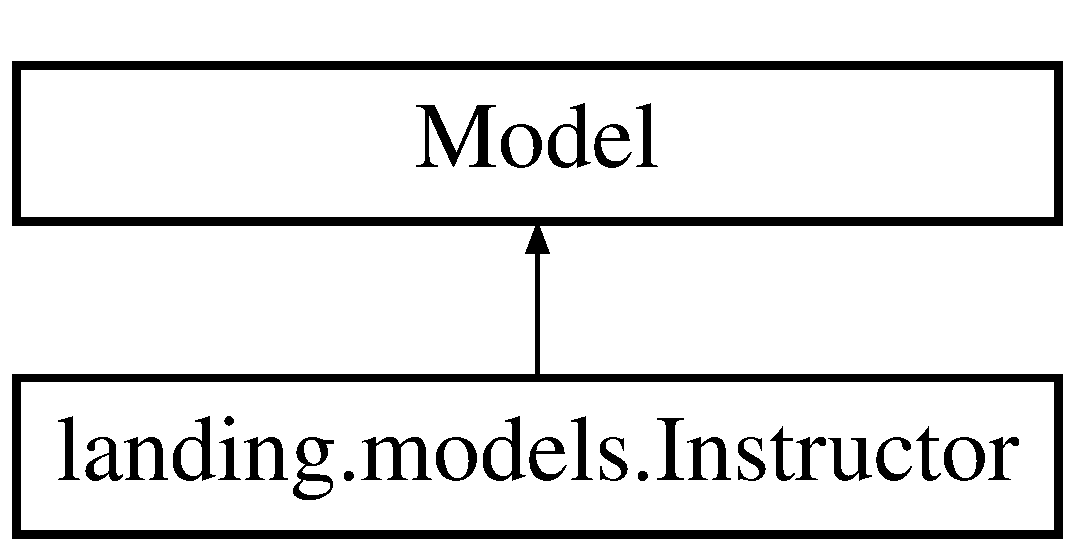
\includegraphics[height=2.000000cm]{classlanding_1_1models_1_1Instructor}
\end{center}
\end{figure}
\subsection*{Static Public Attributes}
\begin{DoxyCompactItemize}
\item 
\mbox{\hyperlink{classlanding_1_1models_1_1Instructor_ad60012a76a46e3ca34f899b073ac3430}{instructor\+\_\+first\+Name}} = models.\+Char\+Field(max\+\_\+length=20)
\item 
\mbox{\hyperlink{classlanding_1_1models_1_1Instructor_a180b4ad797ed2552ab12d29699c56ca6}{instructor\+\_\+last\+Name}} = models.\+Char\+Field(max\+\_\+length=30)
\end{DoxyCompactItemize}


\subsection{Detailed Description}
\begin{DoxyVerb}@Instructor holds what teachers teach a class, this includes the
        instructors first and last name (i.e Harvey Siy),
        This allows for insights on the teachers available for a student to take.
\end{DoxyVerb}
 

Definition at line 114 of file models.\+py.



\subsection{Member Data Documentation}
\mbox{\Hypertarget{classlanding_1_1models_1_1Instructor_ad60012a76a46e3ca34f899b073ac3430}\label{classlanding_1_1models_1_1Instructor_ad60012a76a46e3ca34f899b073ac3430}} 
\index{landing\+::models\+::\+Instructor@{landing\+::models\+::\+Instructor}!instructor\+\_\+first\+Name@{instructor\+\_\+first\+Name}}
\index{instructor\+\_\+first\+Name@{instructor\+\_\+first\+Name}!landing\+::models\+::\+Instructor@{landing\+::models\+::\+Instructor}}
\subsubsection{\texorpdfstring{instructor\+\_\+first\+Name}{instructor\_firstName}}
{\footnotesize\ttfamily landing.\+models.\+Instructor.\+instructor\+\_\+first\+Name = models.\+Char\+Field(max\+\_\+length=20)\hspace{0.3cm}{\ttfamily [static]}}



Definition at line 120 of file models.\+py.

\mbox{\Hypertarget{classlanding_1_1models_1_1Instructor_a180b4ad797ed2552ab12d29699c56ca6}\label{classlanding_1_1models_1_1Instructor_a180b4ad797ed2552ab12d29699c56ca6}} 
\index{landing\+::models\+::\+Instructor@{landing\+::models\+::\+Instructor}!instructor\+\_\+last\+Name@{instructor\+\_\+last\+Name}}
\index{instructor\+\_\+last\+Name@{instructor\+\_\+last\+Name}!landing\+::models\+::\+Instructor@{landing\+::models\+::\+Instructor}}
\subsubsection{\texorpdfstring{instructor\+\_\+last\+Name}{instructor\_lastName}}
{\footnotesize\ttfamily landing.\+models.\+Instructor.\+instructor\+\_\+last\+Name = models.\+Char\+Field(max\+\_\+length=30)\hspace{0.3cm}{\ttfamily [static]}}



Definition at line 121 of file models.\+py.



The documentation for this class was generated from the following file\+:\begin{DoxyCompactItemize}
\item 
mav\+Agenda/landing/\mbox{\hyperlink{models_8py}{models.\+py}}\end{DoxyCompactItemize}

\hypertarget{classlanding_1_1apps_1_1LandingConfig}{}\section{landing.\+apps.\+Landing\+Config Class Reference}
\label{classlanding_1_1apps_1_1LandingConfig}\index{landing.\+apps.\+Landing\+Config@{landing.\+apps.\+Landing\+Config}}
Inheritance diagram for landing.\+apps.\+Landing\+Config\+:\begin{figure}[H]
\begin{center}
\leavevmode
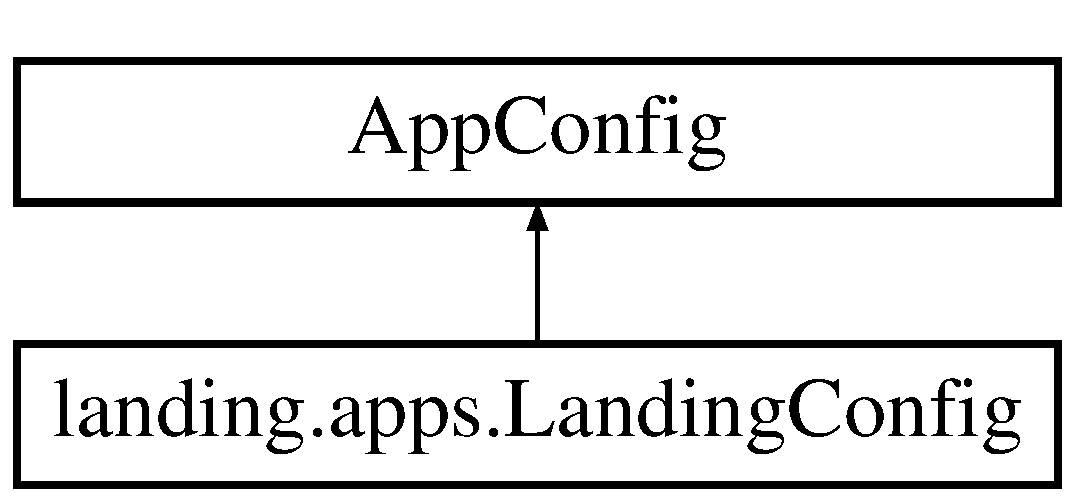
\includegraphics[height=2.000000cm]{classlanding_1_1apps_1_1LandingConfig}
\end{center}
\end{figure}
\subsection*{Static Public Attributes}
\begin{DoxyCompactItemize}
\item 
string \mbox{\hyperlink{classlanding_1_1apps_1_1LandingConfig_a05dc15bad0c66f978227498ad14b2b51}{name}} = \textquotesingle{}landing\textquotesingle{}
\item 
string \mbox{\hyperlink{classlanding_1_1apps_1_1LandingConfig_a5e24228e720bc543458d2f18d457077c}{path}} = \textquotesingle{}/home/py\+Party/Mav\+Link\+Made\+Easy/mav\+Agenda/landing\textquotesingle{}
\end{DoxyCompactItemize}


\subsection{Detailed Description}
\begin{DoxyVerb}@LandingConfig configure attributes of  an application
@param: AppConfig store metadata for application
\end{DoxyVerb}
 

Definition at line 3 of file apps.\+py.



\subsection{Member Data Documentation}
\mbox{\Hypertarget{classlanding_1_1apps_1_1LandingConfig_a05dc15bad0c66f978227498ad14b2b51}\label{classlanding_1_1apps_1_1LandingConfig_a05dc15bad0c66f978227498ad14b2b51}} 
\index{landing\+::apps\+::\+Landing\+Config@{landing\+::apps\+::\+Landing\+Config}!name@{name}}
\index{name@{name}!landing\+::apps\+::\+Landing\+Config@{landing\+::apps\+::\+Landing\+Config}}
\subsubsection{\texorpdfstring{name}{name}}
{\footnotesize\ttfamily string landing.\+apps.\+Landing\+Config.\+name = \textquotesingle{}landing\textquotesingle{}\hspace{0.3cm}{\ttfamily [static]}}



Definition at line 8 of file apps.\+py.

\mbox{\Hypertarget{classlanding_1_1apps_1_1LandingConfig_a5e24228e720bc543458d2f18d457077c}\label{classlanding_1_1apps_1_1LandingConfig_a5e24228e720bc543458d2f18d457077c}} 
\index{landing\+::apps\+::\+Landing\+Config@{landing\+::apps\+::\+Landing\+Config}!path@{path}}
\index{path@{path}!landing\+::apps\+::\+Landing\+Config@{landing\+::apps\+::\+Landing\+Config}}
\subsubsection{\texorpdfstring{path}{path}}
{\footnotesize\ttfamily string landing.\+apps.\+Landing\+Config.\+path = \textquotesingle{}/home/py\+Party/Mav\+Link\+Made\+Easy/mav\+Agenda/landing\textquotesingle{}\hspace{0.3cm}{\ttfamily [static]}}



Definition at line 9 of file apps.\+py.



The documentation for this class was generated from the following file\+:\begin{DoxyCompactItemize}
\item 
mav\+Agenda/landing/\mbox{\hyperlink{apps_8py}{apps.\+py}}\end{DoxyCompactItemize}

\hypertarget{classlanding_1_1forms_1_1UserForm_1_1Meta}{}\section{landing.\+forms.\+User\+Form.\+Meta Class Reference}
\label{classlanding_1_1forms_1_1UserForm_1_1Meta}\index{landing.\+forms.\+User\+Form.\+Meta@{landing.\+forms.\+User\+Form.\+Meta}}
\subsection*{Static Public Attributes}
\begin{DoxyCompactItemize}
\item 
tuple \mbox{\hyperlink{classlanding_1_1forms_1_1UserForm_1_1Meta_a2a26315d592e1403fcc83d8d3437d345}{fields}} = (\textquotesingle{}username\textquotesingle{},\textquotesingle{}password\textquotesingle{},)
\item 
\mbox{\hyperlink{classlanding_1_1forms_1_1UserForm_1_1Meta_ad36e35754db9ad189c731528a0ec160e}{model}} = User
\end{DoxyCompactItemize}


\subsection{Detailed Description}


Definition at line 11 of file forms.\+py.



\subsection{Member Data Documentation}
\mbox{\Hypertarget{classlanding_1_1forms_1_1UserForm_1_1Meta_a2a26315d592e1403fcc83d8d3437d345}\label{classlanding_1_1forms_1_1UserForm_1_1Meta_a2a26315d592e1403fcc83d8d3437d345}} 
\index{landing\+::forms\+::\+User\+Form\+::\+Meta@{landing\+::forms\+::\+User\+Form\+::\+Meta}!fields@{fields}}
\index{fields@{fields}!landing\+::forms\+::\+User\+Form\+::\+Meta@{landing\+::forms\+::\+User\+Form\+::\+Meta}}
\subsubsection{\texorpdfstring{fields}{fields}}
{\footnotesize\ttfamily tuple landing.\+forms.\+User\+Form.\+Meta.\+fields = (\textquotesingle{}username\textquotesingle{},\textquotesingle{}password\textquotesingle{},)\hspace{0.3cm}{\ttfamily [static]}}



Definition at line 13 of file forms.\+py.

\mbox{\Hypertarget{classlanding_1_1forms_1_1UserForm_1_1Meta_ad36e35754db9ad189c731528a0ec160e}\label{classlanding_1_1forms_1_1UserForm_1_1Meta_ad36e35754db9ad189c731528a0ec160e}} 
\index{landing\+::forms\+::\+User\+Form\+::\+Meta@{landing\+::forms\+::\+User\+Form\+::\+Meta}!model@{model}}
\index{model@{model}!landing\+::forms\+::\+User\+Form\+::\+Meta@{landing\+::forms\+::\+User\+Form\+::\+Meta}}
\subsubsection{\texorpdfstring{model}{model}}
{\footnotesize\ttfamily landing.\+forms.\+User\+Form.\+Meta.\+model = User\hspace{0.3cm}{\ttfamily [static]}}



Definition at line 12 of file forms.\+py.



The documentation for this class was generated from the following file\+:\begin{DoxyCompactItemize}
\item 
mav\+Agenda/landing/\mbox{\hyperlink{forms_8py}{forms.\+py}}\end{DoxyCompactItemize}

\hypertarget{classlanding_1_1migrations_1_10001__initial_1_1Migration}{}\section{landing.\+migrations.0001\+\_\+initial.Migration Class Reference}
\label{classlanding_1_1migrations_1_10001__initial_1_1Migration}\index{landing.\+migrations.\+0001\+\_\+initial.\+Migration@{landing.\+migrations.\+0001\+\_\+initial.\+Migration}}
Inheritance diagram for landing.\+migrations.0001\+\_\+initial.Migration\+:\begin{figure}[H]
\begin{center}
\leavevmode
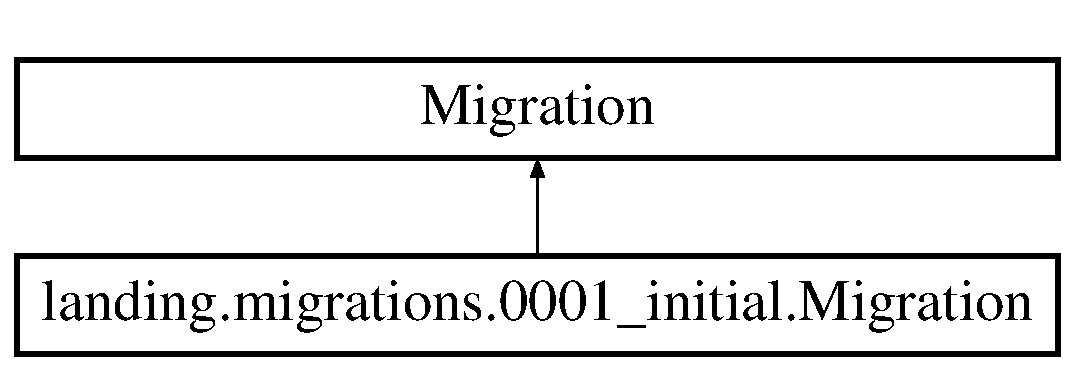
\includegraphics[height=2.000000cm]{classlanding_1_1migrations_1_10001__initial_1_1Migration}
\end{center}
\end{figure}
\subsection*{Static Public Attributes}
\begin{DoxyCompactItemize}
\item 
list \mbox{\hyperlink{classlanding_1_1migrations_1_10001__initial_1_1Migration_a7ae8330b1f6f4c2d840e8988b36a4273}{dependencies}}
\item 
bool \mbox{\hyperlink{classlanding_1_1migrations_1_10001__initial_1_1Migration_a4de7b3a61ec6f60906e74358f823c43c}{initial}} = True
\item 
list \mbox{\hyperlink{classlanding_1_1migrations_1_10001__initial_1_1Migration_abbd7e42fa7ac2174a9fc7593b13b3f23}{operations}}
\end{DoxyCompactItemize}


\subsection{Detailed Description}


Definition at line 8 of file 0001\+\_\+initial.\+py.



\subsection{Member Data Documentation}
\mbox{\Hypertarget{classlanding_1_1migrations_1_10001__initial_1_1Migration_a7ae8330b1f6f4c2d840e8988b36a4273}\label{classlanding_1_1migrations_1_10001__initial_1_1Migration_a7ae8330b1f6f4c2d840e8988b36a4273}} 
\index{landing\+::migrations\+::0001\+\_\+initial\+::\+Migration@{landing\+::migrations\+::0001\+\_\+initial\+::\+Migration}!dependencies@{dependencies}}
\index{dependencies@{dependencies}!landing\+::migrations\+::0001\+\_\+initial\+::\+Migration@{landing\+::migrations\+::0001\+\_\+initial\+::\+Migration}}
\subsubsection{\texorpdfstring{dependencies}{dependencies}}
{\footnotesize\ttfamily list landing.\+migrations.\+0001\+\_\+initial.\+Migration.\+dependencies\hspace{0.3cm}{\ttfamily [static]}}

{\bfseries Initial value\+:}
\begin{DoxyCode}
=  [
        migrations.swappable\_dependency(settings.AUTH\_USER\_MODEL),
    ]
\end{DoxyCode}


Definition at line 12 of file 0001\+\_\+initial.\+py.

\mbox{\Hypertarget{classlanding_1_1migrations_1_10001__initial_1_1Migration_a4de7b3a61ec6f60906e74358f823c43c}\label{classlanding_1_1migrations_1_10001__initial_1_1Migration_a4de7b3a61ec6f60906e74358f823c43c}} 
\index{landing\+::migrations\+::0001\+\_\+initial\+::\+Migration@{landing\+::migrations\+::0001\+\_\+initial\+::\+Migration}!initial@{initial}}
\index{initial@{initial}!landing\+::migrations\+::0001\+\_\+initial\+::\+Migration@{landing\+::migrations\+::0001\+\_\+initial\+::\+Migration}}
\subsubsection{\texorpdfstring{initial}{initial}}
{\footnotesize\ttfamily bool landing.\+migrations.\+0001\+\_\+initial.\+Migration.\+initial = True\hspace{0.3cm}{\ttfamily [static]}}



Definition at line 10 of file 0001\+\_\+initial.\+py.

\mbox{\Hypertarget{classlanding_1_1migrations_1_10001__initial_1_1Migration_abbd7e42fa7ac2174a9fc7593b13b3f23}\label{classlanding_1_1migrations_1_10001__initial_1_1Migration_abbd7e42fa7ac2174a9fc7593b13b3f23}} 
\index{landing\+::migrations\+::0001\+\_\+initial\+::\+Migration@{landing\+::migrations\+::0001\+\_\+initial\+::\+Migration}!operations@{operations}}
\index{operations@{operations}!landing\+::migrations\+::0001\+\_\+initial\+::\+Migration@{landing\+::migrations\+::0001\+\_\+initial\+::\+Migration}}
\subsubsection{\texorpdfstring{operations}{operations}}
{\footnotesize\ttfamily list landing.\+migrations.\+0001\+\_\+initial.\+Migration.\+operations\hspace{0.3cm}{\ttfamily [static]}}



Definition at line 16 of file 0001\+\_\+initial.\+py.



The documentation for this class was generated from the following file\+:\begin{DoxyCompactItemize}
\item 
mav\+Agenda/landing/migrations/\mbox{\hyperlink{0001__initial_8py}{0001\+\_\+initial.\+py}}\end{DoxyCompactItemize}

\hypertarget{classlanding_1_1models_1_1Offering}{}\section{landing.\+models.\+Offering Class Reference}
\label{classlanding_1_1models_1_1Offering}\index{landing.\+models.\+Offering@{landing.\+models.\+Offering}}
Inheritance diagram for landing.\+models.\+Offering\+:\begin{figure}[H]
\begin{center}
\leavevmode
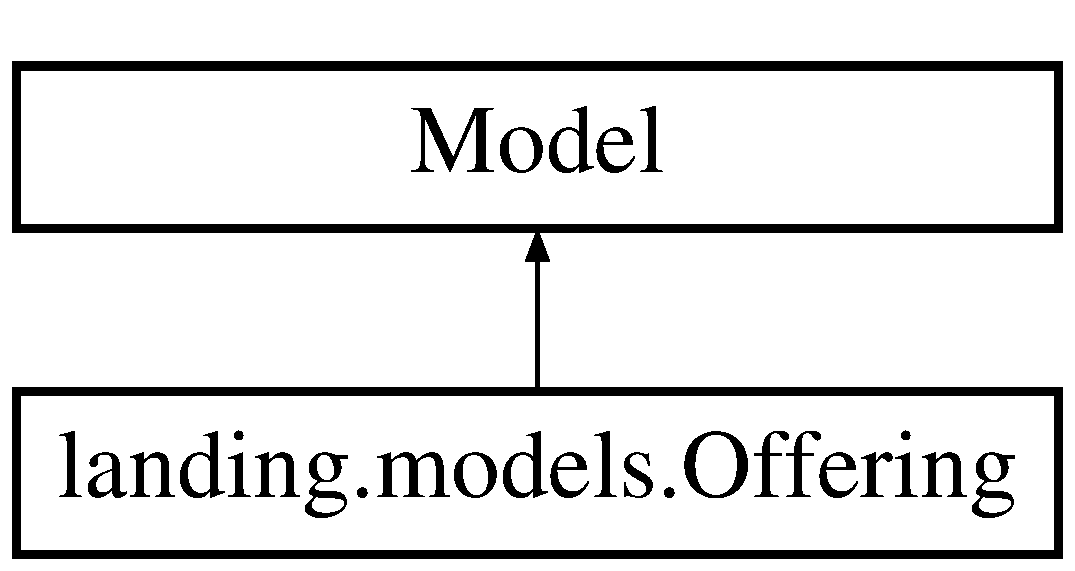
\includegraphics[height=2.000000cm]{classlanding_1_1models_1_1Offering}
\end{center}
\end{figure}
\subsection*{Static Public Attributes}
\begin{DoxyCompactItemize}
\item 
\mbox{\hyperlink{classlanding_1_1models_1_1Offering_a61ee20a63d849a004c9aaa3b8aa00a42}{offering\+\_\+course}} = models.\+Foreign\+Key(\mbox{\hyperlink{classlanding_1_1models_1_1Course}{Course}}, on\+\_\+delete=models.\+C\+A\+S\+C\+A\+DE)
\item 
\mbox{\hyperlink{classlanding_1_1models_1_1Offering_a2680068b2c5f2feb7fe159f59a642d20}{offering\+\_\+days}} = models.\+Many\+To\+Many\+Field(\mbox{\hyperlink{classlanding_1_1models_1_1Weekday}{Weekday}})
\item 
\mbox{\hyperlink{classlanding_1_1models_1_1Offering_a40e7638869d600e27b2d8395f2c0a56b}{offering\+\_\+instructor}} = models.\+Foreign\+Key(\mbox{\hyperlink{classlanding_1_1models_1_1Instructor}{Instructor}}, on\+\_\+delete=models.\+C\+A\+S\+C\+A\+DE)
\item 
\mbox{\hyperlink{classlanding_1_1models_1_1Offering_a4f1b030e6eaefa7b1c869621b4a37f61}{offering\+\_\+location}} = models.\+Foreign\+Key(\mbox{\hyperlink{classlanding_1_1models_1_1Building}{Building}}, on\+\_\+delete=models.\+C\+A\+S\+C\+A\+DE)
\item 
\mbox{\hyperlink{classlanding_1_1models_1_1Offering_a89639b4a5b945918bb4f8a4c08cf8247}{offering\+\_\+section\+Num}} = models.\+Integer\+Field()
\item 
\mbox{\hyperlink{classlanding_1_1models_1_1Offering_a546aca2445d9fabd2dac01b7230f93f5}{offering\+\_\+time}} = models.\+Char\+Field(max\+\_\+length=20)
\end{DoxyCompactItemize}


\subsection{Detailed Description}
\begin{DoxyVerb}@Offering holds the specific class scheduling information labeled above.
        This is not implemented due to time limits given in the Capstone class,
        however, it is coded to show that the application is extensible.
\end{DoxyVerb}
 

Definition at line 147 of file models.\+py.



\subsection{Member Data Documentation}
\mbox{\Hypertarget{classlanding_1_1models_1_1Offering_a61ee20a63d849a004c9aaa3b8aa00a42}\label{classlanding_1_1models_1_1Offering_a61ee20a63d849a004c9aaa3b8aa00a42}} 
\index{landing\+::models\+::\+Offering@{landing\+::models\+::\+Offering}!offering\+\_\+course@{offering\+\_\+course}}
\index{offering\+\_\+course@{offering\+\_\+course}!landing\+::models\+::\+Offering@{landing\+::models\+::\+Offering}}
\subsubsection{\texorpdfstring{offering\+\_\+course}{offering\_course}}
{\footnotesize\ttfamily landing.\+models.\+Offering.\+offering\+\_\+course = models.\+Foreign\+Key(\mbox{\hyperlink{classlanding_1_1models_1_1Course}{Course}}, on\+\_\+delete=models.\+C\+A\+S\+C\+A\+DE)\hspace{0.3cm}{\ttfamily [static]}}



Definition at line 153 of file models.\+py.

\mbox{\Hypertarget{classlanding_1_1models_1_1Offering_a2680068b2c5f2feb7fe159f59a642d20}\label{classlanding_1_1models_1_1Offering_a2680068b2c5f2feb7fe159f59a642d20}} 
\index{landing\+::models\+::\+Offering@{landing\+::models\+::\+Offering}!offering\+\_\+days@{offering\+\_\+days}}
\index{offering\+\_\+days@{offering\+\_\+days}!landing\+::models\+::\+Offering@{landing\+::models\+::\+Offering}}
\subsubsection{\texorpdfstring{offering\+\_\+days}{offering\_days}}
{\footnotesize\ttfamily landing.\+models.\+Offering.\+offering\+\_\+days = models.\+Many\+To\+Many\+Field(\mbox{\hyperlink{classlanding_1_1models_1_1Weekday}{Weekday}})\hspace{0.3cm}{\ttfamily [static]}}



Definition at line 156 of file models.\+py.

\mbox{\Hypertarget{classlanding_1_1models_1_1Offering_a40e7638869d600e27b2d8395f2c0a56b}\label{classlanding_1_1models_1_1Offering_a40e7638869d600e27b2d8395f2c0a56b}} 
\index{landing\+::models\+::\+Offering@{landing\+::models\+::\+Offering}!offering\+\_\+instructor@{offering\+\_\+instructor}}
\index{offering\+\_\+instructor@{offering\+\_\+instructor}!landing\+::models\+::\+Offering@{landing\+::models\+::\+Offering}}
\subsubsection{\texorpdfstring{offering\+\_\+instructor}{offering\_instructor}}
{\footnotesize\ttfamily landing.\+models.\+Offering.\+offering\+\_\+instructor = models.\+Foreign\+Key(\mbox{\hyperlink{classlanding_1_1models_1_1Instructor}{Instructor}}, on\+\_\+delete=models.\+C\+A\+S\+C\+A\+DE)\hspace{0.3cm}{\ttfamily [static]}}



Definition at line 158 of file models.\+py.

\mbox{\Hypertarget{classlanding_1_1models_1_1Offering_a4f1b030e6eaefa7b1c869621b4a37f61}\label{classlanding_1_1models_1_1Offering_a4f1b030e6eaefa7b1c869621b4a37f61}} 
\index{landing\+::models\+::\+Offering@{landing\+::models\+::\+Offering}!offering\+\_\+location@{offering\+\_\+location}}
\index{offering\+\_\+location@{offering\+\_\+location}!landing\+::models\+::\+Offering@{landing\+::models\+::\+Offering}}
\subsubsection{\texorpdfstring{offering\+\_\+location}{offering\_location}}
{\footnotesize\ttfamily landing.\+models.\+Offering.\+offering\+\_\+location = models.\+Foreign\+Key(\mbox{\hyperlink{classlanding_1_1models_1_1Building}{Building}}, on\+\_\+delete=models.\+C\+A\+S\+C\+A\+DE)\hspace{0.3cm}{\ttfamily [static]}}



Definition at line 155 of file models.\+py.

\mbox{\Hypertarget{classlanding_1_1models_1_1Offering_a89639b4a5b945918bb4f8a4c08cf8247}\label{classlanding_1_1models_1_1Offering_a89639b4a5b945918bb4f8a4c08cf8247}} 
\index{landing\+::models\+::\+Offering@{landing\+::models\+::\+Offering}!offering\+\_\+section\+Num@{offering\+\_\+section\+Num}}
\index{offering\+\_\+section\+Num@{offering\+\_\+section\+Num}!landing\+::models\+::\+Offering@{landing\+::models\+::\+Offering}}
\subsubsection{\texorpdfstring{offering\+\_\+section\+Num}{offering\_sectionNum}}
{\footnotesize\ttfamily landing.\+models.\+Offering.\+offering\+\_\+section\+Num = models.\+Integer\+Field()\hspace{0.3cm}{\ttfamily [static]}}



Definition at line 157 of file models.\+py.

\mbox{\Hypertarget{classlanding_1_1models_1_1Offering_a546aca2445d9fabd2dac01b7230f93f5}\label{classlanding_1_1models_1_1Offering_a546aca2445d9fabd2dac01b7230f93f5}} 
\index{landing\+::models\+::\+Offering@{landing\+::models\+::\+Offering}!offering\+\_\+time@{offering\+\_\+time}}
\index{offering\+\_\+time@{offering\+\_\+time}!landing\+::models\+::\+Offering@{landing\+::models\+::\+Offering}}
\subsubsection{\texorpdfstring{offering\+\_\+time}{offering\_time}}
{\footnotesize\ttfamily landing.\+models.\+Offering.\+offering\+\_\+time = models.\+Char\+Field(max\+\_\+length=20)\hspace{0.3cm}{\ttfamily [static]}}



Definition at line 154 of file models.\+py.



The documentation for this class was generated from the following file\+:\begin{DoxyCompactItemize}
\item 
mav\+Agenda/landing/\mbox{\hyperlink{models_8py}{models.\+py}}\end{DoxyCompactItemize}

\hypertarget{classlanding_1_1models_1_1Prereq}{}\section{landing.\+models.\+Prereq Class Reference}
\label{classlanding_1_1models_1_1Prereq}\index{landing.\+models.\+Prereq@{landing.\+models.\+Prereq}}
Inheritance diagram for landing.\+models.\+Prereq\+:\begin{figure}[H]
\begin{center}
\leavevmode
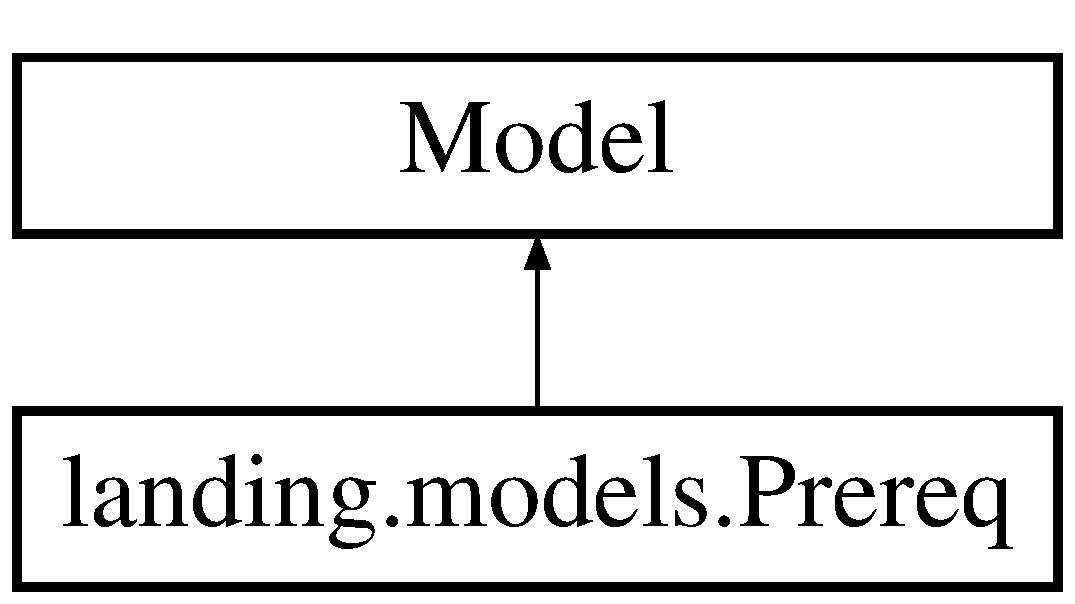
\includegraphics[height=2.000000cm]{classlanding_1_1models_1_1Prereq}
\end{center}
\end{figure}
\subsection*{Static Public Attributes}
\begin{DoxyCompactItemize}
\item 
string \mbox{\hyperlink{classlanding_1_1models_1_1Prereq_ab8f9e1e86370dc76c689d122c2910982}{C}} = \char`\"{}Corequisite\char`\"{}
\item 
string \mbox{\hyperlink{classlanding_1_1models_1_1Prereq_ab99082a563d5a9e30793d92d38cf4b5a}{P}} = \char`\"{}Prerequisite\char`\"{}
\item 
\mbox{\hyperlink{classlanding_1_1models_1_1Prereq_a4e83c57d21589b742a3bd537e64c9263}{prereq\+\_\+courses}} = models.\+Many\+To\+Many\+Field(\mbox{\hyperlink{classlanding_1_1models_1_1Course}{Course}})
\item 
\mbox{\hyperlink{classlanding_1_1models_1_1Prereq_a32ccec77ab248409d6aecb58de5d57bb}{prereq\+\_\+type}} = models.\+Char\+Field(max\+\_\+length=20, choices=\mbox{\hyperlink{classlanding_1_1models_1_1Prereq_a04e7ec750245a108149ff8680c846509}{R\+E\+Q\+\_\+\+C\+H\+O\+I\+CE}}, null=True)
\item 
tuple \mbox{\hyperlink{classlanding_1_1models_1_1Prereq_a04e7ec750245a108149ff8680c846509}{R\+E\+Q\+\_\+\+C\+H\+O\+I\+CE}}
\end{DoxyCompactItemize}


\subsection{Detailed Description}
\begin{DoxyVerb}@Prereq  holds classes that are prerequisites to other classes,
        this includes the type (i.e Corequisite or Prerequisite) and a foreign key reference
        back to the Course table.
\end{DoxyVerb}
 

Definition at line 160 of file models.\+py.



\subsection{Member Data Documentation}
\mbox{\Hypertarget{classlanding_1_1models_1_1Prereq_ab8f9e1e86370dc76c689d122c2910982}\label{classlanding_1_1models_1_1Prereq_ab8f9e1e86370dc76c689d122c2910982}} 
\index{landing\+::models\+::\+Prereq@{landing\+::models\+::\+Prereq}!C@{C}}
\index{C@{C}!landing\+::models\+::\+Prereq@{landing\+::models\+::\+Prereq}}
\subsubsection{\texorpdfstring{C}{C}}
{\footnotesize\ttfamily string landing.\+models.\+Prereq.\+C = \char`\"{}Corequisite\char`\"{}\hspace{0.3cm}{\ttfamily [static]}}



Definition at line 166 of file models.\+py.

\mbox{\Hypertarget{classlanding_1_1models_1_1Prereq_ab99082a563d5a9e30793d92d38cf4b5a}\label{classlanding_1_1models_1_1Prereq_ab99082a563d5a9e30793d92d38cf4b5a}} 
\index{landing\+::models\+::\+Prereq@{landing\+::models\+::\+Prereq}!P@{P}}
\index{P@{P}!landing\+::models\+::\+Prereq@{landing\+::models\+::\+Prereq}}
\subsubsection{\texorpdfstring{P}{P}}
{\footnotesize\ttfamily string landing.\+models.\+Prereq.\+P = \char`\"{}Prerequisite\char`\"{}\hspace{0.3cm}{\ttfamily [static]}}



Definition at line 167 of file models.\+py.

\mbox{\Hypertarget{classlanding_1_1models_1_1Prereq_a4e83c57d21589b742a3bd537e64c9263}\label{classlanding_1_1models_1_1Prereq_a4e83c57d21589b742a3bd537e64c9263}} 
\index{landing\+::models\+::\+Prereq@{landing\+::models\+::\+Prereq}!prereq\+\_\+courses@{prereq\+\_\+courses}}
\index{prereq\+\_\+courses@{prereq\+\_\+courses}!landing\+::models\+::\+Prereq@{landing\+::models\+::\+Prereq}}
\subsubsection{\texorpdfstring{prereq\+\_\+courses}{prereq\_courses}}
{\footnotesize\ttfamily landing.\+models.\+Prereq.\+prereq\+\_\+courses = models.\+Many\+To\+Many\+Field(\mbox{\hyperlink{classlanding_1_1models_1_1Course}{Course}})\hspace{0.3cm}{\ttfamily [static]}}



Definition at line 173 of file models.\+py.

\mbox{\Hypertarget{classlanding_1_1models_1_1Prereq_a32ccec77ab248409d6aecb58de5d57bb}\label{classlanding_1_1models_1_1Prereq_a32ccec77ab248409d6aecb58de5d57bb}} 
\index{landing\+::models\+::\+Prereq@{landing\+::models\+::\+Prereq}!prereq\+\_\+type@{prereq\+\_\+type}}
\index{prereq\+\_\+type@{prereq\+\_\+type}!landing\+::models\+::\+Prereq@{landing\+::models\+::\+Prereq}}
\subsubsection{\texorpdfstring{prereq\+\_\+type}{prereq\_type}}
{\footnotesize\ttfamily landing.\+models.\+Prereq.\+prereq\+\_\+type = models.\+Char\+Field(max\+\_\+length=20, choices=\mbox{\hyperlink{classlanding_1_1models_1_1Prereq_a04e7ec750245a108149ff8680c846509}{R\+E\+Q\+\_\+\+C\+H\+O\+I\+CE}}, null=True)\hspace{0.3cm}{\ttfamily [static]}}



Definition at line 172 of file models.\+py.

\mbox{\Hypertarget{classlanding_1_1models_1_1Prereq_a04e7ec750245a108149ff8680c846509}\label{classlanding_1_1models_1_1Prereq_a04e7ec750245a108149ff8680c846509}} 
\index{landing\+::models\+::\+Prereq@{landing\+::models\+::\+Prereq}!R\+E\+Q\+\_\+\+C\+H\+O\+I\+CE@{R\+E\+Q\+\_\+\+C\+H\+O\+I\+CE}}
\index{R\+E\+Q\+\_\+\+C\+H\+O\+I\+CE@{R\+E\+Q\+\_\+\+C\+H\+O\+I\+CE}!landing\+::models\+::\+Prereq@{landing\+::models\+::\+Prereq}}
\subsubsection{\texorpdfstring{R\+E\+Q\+\_\+\+C\+H\+O\+I\+CE}{REQ\_CHOICE}}
{\footnotesize\ttfamily tuple landing.\+models.\+Prereq.\+R\+E\+Q\+\_\+\+C\+H\+O\+I\+CE\hspace{0.3cm}{\ttfamily [static]}}

{\bfseries Initial value\+:}
\begin{DoxyCode}
=  (
        (C, \textcolor{stringliteral}{"Corequisite"}),
        (P, \textcolor{stringliteral}{"Prerequisite"}),
    )
\end{DoxyCode}


Definition at line 168 of file models.\+py.



The documentation for this class was generated from the following file\+:\begin{DoxyCompactItemize}
\item 
mav\+Agenda/landing/\mbox{\hyperlink{models_8py}{models.\+py}}\end{DoxyCompactItemize}

\hypertarget{classlanding_1_1models_1_1Requirement}{}\section{landing.\+models.\+Requirement Class Reference}
\label{classlanding_1_1models_1_1Requirement}\index{landing.\+models.\+Requirement@{landing.\+models.\+Requirement}}
Inheritance diagram for landing.\+models.\+Requirement\+:\begin{figure}[H]
\begin{center}
\leavevmode
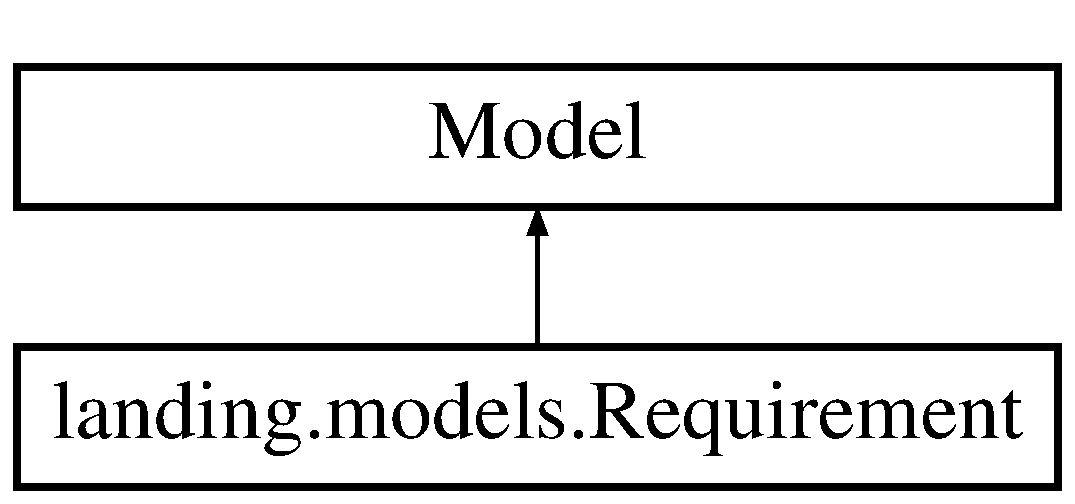
\includegraphics[height=2.000000cm]{classlanding_1_1models_1_1Requirement}
\end{center}
\end{figure}
\subsection*{Static Public Attributes}
\begin{DoxyCompactItemize}
\item 
\mbox{\hyperlink{classlanding_1_1models_1_1Requirement_a89e4f0cb28049b5e23d26f96bf23fe1b}{req\+\_\+credits}} = models.\+Integer\+Field()
\item 
\mbox{\hyperlink{classlanding_1_1models_1_1Requirement_a1308b8c10928402f769fddebf28dd05c}{req\+\_\+degrees}} = models.\+Many\+To\+Many\+Field(\mbox{\hyperlink{classlanding_1_1models_1_1Degree}{Degree}})
\item 
\mbox{\hyperlink{classlanding_1_1models_1_1Requirement_aae1f2fa53a3240a83cf827b942ac2ef2}{req\+\_\+name}} = models.\+Char\+Field(max\+\_\+length=50)
\end{DoxyCompactItemize}


\subsection{Detailed Description}
\begin{DoxyVerb}@Requirement holds the required classes for a specific degree, this includes the
        name (i.e Java 1), credits (i.e. 3),
        and degrees (i.e. Bachelor of Science, Major, Computer Science).
\end{DoxyVerb}
 

Definition at line 43 of file models.\+py.



\subsection{Member Data Documentation}
\mbox{\Hypertarget{classlanding_1_1models_1_1Requirement_a89e4f0cb28049b5e23d26f96bf23fe1b}\label{classlanding_1_1models_1_1Requirement_a89e4f0cb28049b5e23d26f96bf23fe1b}} 
\index{landing\+::models\+::\+Requirement@{landing\+::models\+::\+Requirement}!req\+\_\+credits@{req\+\_\+credits}}
\index{req\+\_\+credits@{req\+\_\+credits}!landing\+::models\+::\+Requirement@{landing\+::models\+::\+Requirement}}
\subsubsection{\texorpdfstring{req\+\_\+credits}{req\_credits}}
{\footnotesize\ttfamily landing.\+models.\+Requirement.\+req\+\_\+credits = models.\+Integer\+Field()\hspace{0.3cm}{\ttfamily [static]}}



Definition at line 50 of file models.\+py.

\mbox{\Hypertarget{classlanding_1_1models_1_1Requirement_a1308b8c10928402f769fddebf28dd05c}\label{classlanding_1_1models_1_1Requirement_a1308b8c10928402f769fddebf28dd05c}} 
\index{landing\+::models\+::\+Requirement@{landing\+::models\+::\+Requirement}!req\+\_\+degrees@{req\+\_\+degrees}}
\index{req\+\_\+degrees@{req\+\_\+degrees}!landing\+::models\+::\+Requirement@{landing\+::models\+::\+Requirement}}
\subsubsection{\texorpdfstring{req\+\_\+degrees}{req\_degrees}}
{\footnotesize\ttfamily landing.\+models.\+Requirement.\+req\+\_\+degrees = models.\+Many\+To\+Many\+Field(\mbox{\hyperlink{classlanding_1_1models_1_1Degree}{Degree}})\hspace{0.3cm}{\ttfamily [static]}}



Definition at line 51 of file models.\+py.

\mbox{\Hypertarget{classlanding_1_1models_1_1Requirement_aae1f2fa53a3240a83cf827b942ac2ef2}\label{classlanding_1_1models_1_1Requirement_aae1f2fa53a3240a83cf827b942ac2ef2}} 
\index{landing\+::models\+::\+Requirement@{landing\+::models\+::\+Requirement}!req\+\_\+name@{req\+\_\+name}}
\index{req\+\_\+name@{req\+\_\+name}!landing\+::models\+::\+Requirement@{landing\+::models\+::\+Requirement}}
\subsubsection{\texorpdfstring{req\+\_\+name}{req\_name}}
{\footnotesize\ttfamily landing.\+models.\+Requirement.\+req\+\_\+name = models.\+Char\+Field(max\+\_\+length=50)\hspace{0.3cm}{\ttfamily [static]}}



Definition at line 49 of file models.\+py.



The documentation for this class was generated from the following file\+:\begin{DoxyCompactItemize}
\item 
mav\+Agenda/landing/\mbox{\hyperlink{models_8py}{models.\+py}}\end{DoxyCompactItemize}

\hypertarget{classlanding_1_1tests_1_1test__UI_1_1UITests}{}\section{landing.\+tests.\+test\+\_\+\+U\+I.\+U\+I\+Tests Class Reference}
\label{classlanding_1_1tests_1_1test__UI_1_1UITests}\index{landing.\+tests.\+test\+\_\+\+U\+I.\+U\+I\+Tests@{landing.\+tests.\+test\+\_\+\+U\+I.\+U\+I\+Tests}}
Inheritance diagram for landing.\+tests.\+test\+\_\+\+U\+I.\+U\+I\+Tests\+:\begin{figure}[H]
\begin{center}
\leavevmode
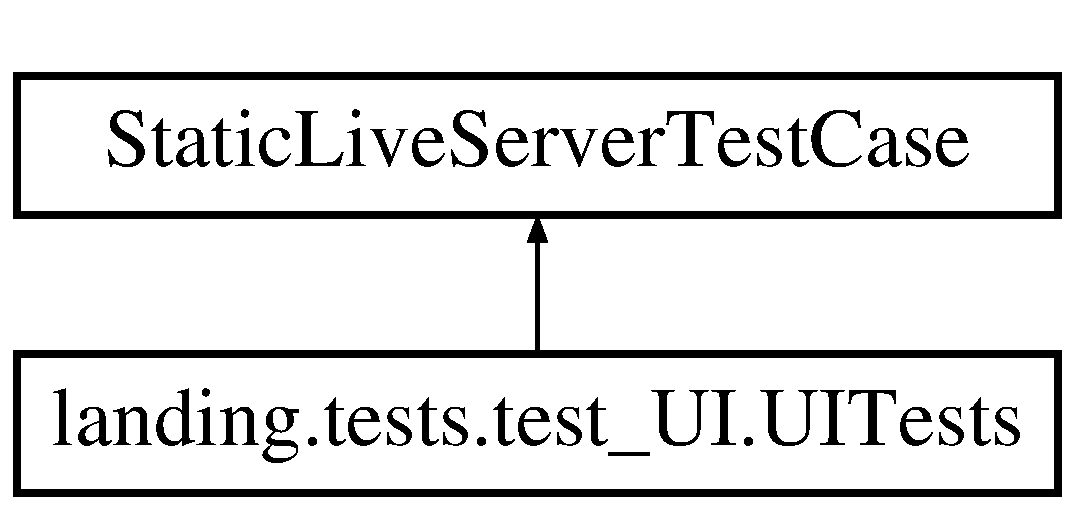
\includegraphics[height=2.000000cm]{classlanding_1_1tests_1_1test__UI_1_1UITests}
\end{center}
\end{figure}
\subsection*{Public Member Functions}
\begin{DoxyCompactItemize}
\item 
def \mbox{\hyperlink{classlanding_1_1tests_1_1test__UI_1_1UITests_a63dc03589cdac58df8716fbb1fb3279b}{set\+Up\+Class}} (cls)
\item 
def \mbox{\hyperlink{classlanding_1_1tests_1_1test__UI_1_1UITests_a2d3a96bc34095bed7567d567563e8d82}{tear\+Down\+Class}} (cls)
\item 
def \mbox{\hyperlink{classlanding_1_1tests_1_1test__UI_1_1UITests_ac3d481487cc39ef72303722c3fd779d7}{test\+\_\+addclasses\+\_\+form}} (self)
\item 
def \mbox{\hyperlink{classlanding_1_1tests_1_1test__UI_1_1UITests_a97adaea38b64567b0757f65c31770044}{test\+\_\+createuser\+\_\+form}} (self)
\item 
def \mbox{\hyperlink{classlanding_1_1tests_1_1test__UI_1_1UITests_a2d1e2011a8c152e486dc0c415797fdc9}{test\+\_\+selectcourses\+\_\+form}} (self)
\end{DoxyCompactItemize}
\subsection*{Public Attributes}
\begin{DoxyCompactItemize}
\item 
\mbox{\hyperlink{classlanding_1_1tests_1_1test__UI_1_1UITests_a71f844dbde9cf4cf3b0a74dcbe13bdd9}{selenium}}
\end{DoxyCompactItemize}


\subsection{Detailed Description}
\begin{DoxyVerb}@UITests contain all of the classes that relate to performing actions on UI elements (i.e. buttons)
param: StaticLiveServerTestCase allows for automated testing
at execution time by launching a server in the background &
shuts it down on teardown
\end{DoxyVerb}
 

Definition at line 9 of file test\+\_\+\+U\+I.\+py.



\subsection{Member Function Documentation}
\mbox{\Hypertarget{classlanding_1_1tests_1_1test__UI_1_1UITests_a63dc03589cdac58df8716fbb1fb3279b}\label{classlanding_1_1tests_1_1test__UI_1_1UITests_a63dc03589cdac58df8716fbb1fb3279b}} 
\index{landing\+::tests\+::test\+\_\+\+U\+I\+::\+U\+I\+Tests@{landing\+::tests\+::test\+\_\+\+U\+I\+::\+U\+I\+Tests}!set\+Up\+Class@{set\+Up\+Class}}
\index{set\+Up\+Class@{set\+Up\+Class}!landing\+::tests\+::test\+\_\+\+U\+I\+::\+U\+I\+Tests@{landing\+::tests\+::test\+\_\+\+U\+I\+::\+U\+I\+Tests}}
\subsubsection{\texorpdfstring{set\+Up\+Class()}{setUpClass()}}
{\footnotesize\ttfamily def landing.\+tests.\+test\+\_\+\+U\+I.\+U\+I\+Tests.\+set\+Up\+Class (\begin{DoxyParamCaption}\item[{}]{cls }\end{DoxyParamCaption})}



Definition at line 18 of file test\+\_\+\+U\+I.\+py.

\mbox{\Hypertarget{classlanding_1_1tests_1_1test__UI_1_1UITests_a2d3a96bc34095bed7567d567563e8d82}\label{classlanding_1_1tests_1_1test__UI_1_1UITests_a2d3a96bc34095bed7567d567563e8d82}} 
\index{landing\+::tests\+::test\+\_\+\+U\+I\+::\+U\+I\+Tests@{landing\+::tests\+::test\+\_\+\+U\+I\+::\+U\+I\+Tests}!tear\+Down\+Class@{tear\+Down\+Class}}
\index{tear\+Down\+Class@{tear\+Down\+Class}!landing\+::tests\+::test\+\_\+\+U\+I\+::\+U\+I\+Tests@{landing\+::tests\+::test\+\_\+\+U\+I\+::\+U\+I\+Tests}}
\subsubsection{\texorpdfstring{tear\+Down\+Class()}{tearDownClass()}}
{\footnotesize\ttfamily def landing.\+tests.\+test\+\_\+\+U\+I.\+U\+I\+Tests.\+tear\+Down\+Class (\begin{DoxyParamCaption}\item[{}]{cls }\end{DoxyParamCaption})}



Definition at line 23 of file test\+\_\+\+U\+I.\+py.



References landing.\+tests.\+test\+\_\+\+U\+I.\+U\+I\+Tests.\+selenium.

\mbox{\Hypertarget{classlanding_1_1tests_1_1test__UI_1_1UITests_ac3d481487cc39ef72303722c3fd779d7}\label{classlanding_1_1tests_1_1test__UI_1_1UITests_ac3d481487cc39ef72303722c3fd779d7}} 
\index{landing\+::tests\+::test\+\_\+\+U\+I\+::\+U\+I\+Tests@{landing\+::tests\+::test\+\_\+\+U\+I\+::\+U\+I\+Tests}!test\+\_\+addclasses\+\_\+form@{test\+\_\+addclasses\+\_\+form}}
\index{test\+\_\+addclasses\+\_\+form@{test\+\_\+addclasses\+\_\+form}!landing\+::tests\+::test\+\_\+\+U\+I\+::\+U\+I\+Tests@{landing\+::tests\+::test\+\_\+\+U\+I\+::\+U\+I\+Tests}}
\subsubsection{\texorpdfstring{test\+\_\+addclasses\+\_\+form()}{test\_addclasses\_form()}}
{\footnotesize\ttfamily def landing.\+tests.\+test\+\_\+\+U\+I.\+U\+I\+Tests.\+test\+\_\+addclasses\+\_\+form (\begin{DoxyParamCaption}\item[{}]{self }\end{DoxyParamCaption})}



Definition at line 41 of file test\+\_\+\+U\+I.\+py.



References landing.\+tests.\+test\+\_\+\+U\+I.\+U\+I\+Tests.\+selenium.

\mbox{\Hypertarget{classlanding_1_1tests_1_1test__UI_1_1UITests_a97adaea38b64567b0757f65c31770044}\label{classlanding_1_1tests_1_1test__UI_1_1UITests_a97adaea38b64567b0757f65c31770044}} 
\index{landing\+::tests\+::test\+\_\+\+U\+I\+::\+U\+I\+Tests@{landing\+::tests\+::test\+\_\+\+U\+I\+::\+U\+I\+Tests}!test\+\_\+createuser\+\_\+form@{test\+\_\+createuser\+\_\+form}}
\index{test\+\_\+createuser\+\_\+form@{test\+\_\+createuser\+\_\+form}!landing\+::tests\+::test\+\_\+\+U\+I\+::\+U\+I\+Tests@{landing\+::tests\+::test\+\_\+\+U\+I\+::\+U\+I\+Tests}}
\subsubsection{\texorpdfstring{test\+\_\+createuser\+\_\+form()}{test\_createuser\_form()}}
{\footnotesize\ttfamily def landing.\+tests.\+test\+\_\+\+U\+I.\+U\+I\+Tests.\+test\+\_\+createuser\+\_\+form (\begin{DoxyParamCaption}\item[{}]{self }\end{DoxyParamCaption})}



Definition at line 26 of file test\+\_\+\+U\+I.\+py.



References landing.\+tests.\+test\+\_\+\+U\+I.\+U\+I\+Tests.\+selenium.

\mbox{\Hypertarget{classlanding_1_1tests_1_1test__UI_1_1UITests_a2d1e2011a8c152e486dc0c415797fdc9}\label{classlanding_1_1tests_1_1test__UI_1_1UITests_a2d1e2011a8c152e486dc0c415797fdc9}} 
\index{landing\+::tests\+::test\+\_\+\+U\+I\+::\+U\+I\+Tests@{landing\+::tests\+::test\+\_\+\+U\+I\+::\+U\+I\+Tests}!test\+\_\+selectcourses\+\_\+form@{test\+\_\+selectcourses\+\_\+form}}
\index{test\+\_\+selectcourses\+\_\+form@{test\+\_\+selectcourses\+\_\+form}!landing\+::tests\+::test\+\_\+\+U\+I\+::\+U\+I\+Tests@{landing\+::tests\+::test\+\_\+\+U\+I\+::\+U\+I\+Tests}}
\subsubsection{\texorpdfstring{test\+\_\+selectcourses\+\_\+form()}{test\_selectcourses\_form()}}
{\footnotesize\ttfamily def landing.\+tests.\+test\+\_\+\+U\+I.\+U\+I\+Tests.\+test\+\_\+selectcourses\+\_\+form (\begin{DoxyParamCaption}\item[{}]{self }\end{DoxyParamCaption})}



Definition at line 35 of file test\+\_\+\+U\+I.\+py.



References landing.\+tests.\+test\+\_\+\+U\+I.\+U\+I\+Tests.\+selenium.



\subsection{Member Data Documentation}
\mbox{\Hypertarget{classlanding_1_1tests_1_1test__UI_1_1UITests_a71f844dbde9cf4cf3b0a74dcbe13bdd9}\label{classlanding_1_1tests_1_1test__UI_1_1UITests_a71f844dbde9cf4cf3b0a74dcbe13bdd9}} 
\index{landing\+::tests\+::test\+\_\+\+U\+I\+::\+U\+I\+Tests@{landing\+::tests\+::test\+\_\+\+U\+I\+::\+U\+I\+Tests}!selenium@{selenium}}
\index{selenium@{selenium}!landing\+::tests\+::test\+\_\+\+U\+I\+::\+U\+I\+Tests@{landing\+::tests\+::test\+\_\+\+U\+I\+::\+U\+I\+Tests}}
\subsubsection{\texorpdfstring{selenium}{selenium}}
{\footnotesize\ttfamily landing.\+tests.\+test\+\_\+\+U\+I.\+U\+I\+Tests.\+selenium}



Definition at line 19 of file test\+\_\+\+U\+I.\+py.



Referenced by landing.\+tests.\+test\+\_\+\+U\+I.\+U\+I\+Tests.\+tear\+Down\+Class(), landing.\+tests.\+test\+\_\+\+U\+I.\+U\+I\+Tests.\+test\+\_\+addclasses\+\_\+form(), landing.\+tests.\+test\+\_\+\+U\+I.\+U\+I\+Tests.\+test\+\_\+createuser\+\_\+form(), and landing.\+tests.\+test\+\_\+\+U\+I.\+U\+I\+Tests.\+test\+\_\+selectcourses\+\_\+form().



The documentation for this class was generated from the following file\+:\begin{DoxyCompactItemize}
\item 
mav\+Agenda/landing/tests/\mbox{\hyperlink{test__UI_8py}{test\+\_\+\+U\+I.\+py}}\end{DoxyCompactItemize}

\hypertarget{classlanding_1_1forms_1_1UserForm}{}\section{landing.\+forms.\+User\+Form Class Reference}
\label{classlanding_1_1forms_1_1UserForm}\index{landing.\+forms.\+User\+Form@{landing.\+forms.\+User\+Form}}
Inheritance diagram for landing.\+forms.\+User\+Form\+:\begin{figure}[H]
\begin{center}
\leavevmode
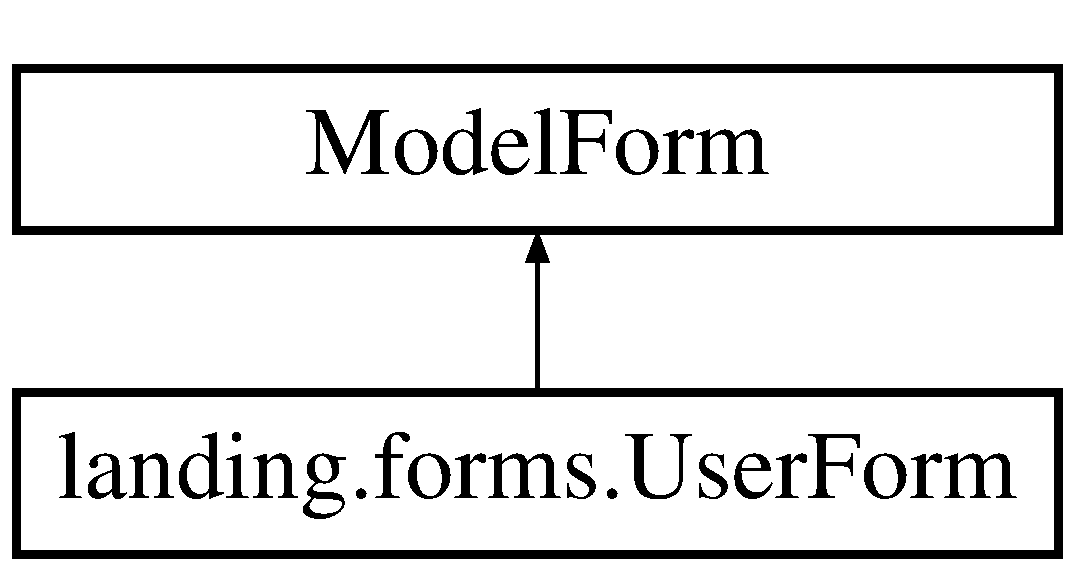
\includegraphics[height=2.000000cm]{classlanding_1_1forms_1_1UserForm}
\end{center}
\end{figure}
\subsection*{Classes}
\begin{DoxyCompactItemize}
\item 
class \mbox{\hyperlink{classlanding_1_1forms_1_1UserForm_1_1Meta}{Meta}}
\end{DoxyCompactItemize}


\subsection{Detailed Description}
\begin{DoxyVerb}@EmailForm collection of fields to allow for user login with email address
@forms.Form: associated data within fields
\end{DoxyVerb}
 

Definition at line 6 of file forms.\+py.



The documentation for this class was generated from the following file\+:\begin{DoxyCompactItemize}
\item 
mav\+Agenda/landing/\mbox{\hyperlink{forms_8py}{forms.\+py}}\end{DoxyCompactItemize}

\hypertarget{classlanding_1_1models_1_1UserPreferences}{}\section{landing.\+models.\+User\+Preferences Class Reference}
\label{classlanding_1_1models_1_1UserPreferences}\index{landing.\+models.\+User\+Preferences@{landing.\+models.\+User\+Preferences}}
Inheritance diagram for landing.\+models.\+User\+Preferences\+:\begin{figure}[H]
\begin{center}
\leavevmode
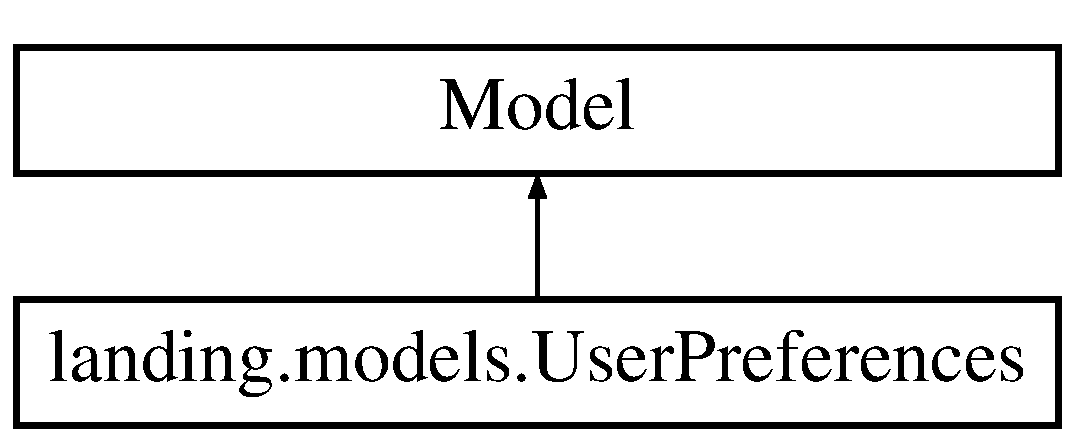
\includegraphics[height=2.000000cm]{classlanding_1_1models_1_1UserPreferences}
\end{center}
\end{figure}
\subsection*{Static Public Attributes}
\begin{DoxyCompactItemize}
\item 
\mbox{\hyperlink{classlanding_1_1models_1_1UserPreferences_a01a3066ef3e14f95e7749494de25e698}{pref\+\_\+max\+Credits}} = models.\+Integer\+Field()
\item 
\mbox{\hyperlink{classlanding_1_1models_1_1UserPreferences_a7f5982f807cfd77d3e54369e807cbbbf}{pref\+\_\+min\+Credits}} = models.\+Integer\+Field()
\item 
\mbox{\hyperlink{classlanding_1_1models_1_1UserPreferences_a8ff382133c91bf0c8775c98d6167e570}{pref\+\_\+next\+Sem\+Max\+Credit}} = models.\+Integer\+Field(null=True)
\item 
\mbox{\hyperlink{classlanding_1_1models_1_1UserPreferences_a29c59f4202078df42d2b36004ddd42ef}{pref\+\_\+next\+Sem\+Min\+Credit}} = models.\+Integer\+Field(null=True)
\item 
\mbox{\hyperlink{classlanding_1_1models_1_1UserPreferences_a1bca302f110047fa3c4ddb92a72e93b1}{pref\+\_\+next\+S\+SF}} = models.\+Char\+Field(max\+\_\+length=10, null=True)
\item 
\mbox{\hyperlink{classlanding_1_1models_1_1UserPreferences_a5ca4985a674bd12b3e1749779ecc7024}{pref\+\_\+next\+Year}} = models.\+Integer\+Field(null=True)
\item 
\mbox{\hyperlink{classlanding_1_1models_1_1UserPreferences_a4aaacfc3aa258135e00af12c6ec4d09f}{pref\+\_\+summer}} = models.\+Boolean\+Field()
\item 
\mbox{\hyperlink{classlanding_1_1models_1_1UserPreferences_aa092d2329abff89f22e57a07959ddad5}{pref\+\_\+summer\+Max\+Credits}} = models.\+Integer\+Field()
\item 
\mbox{\hyperlink{classlanding_1_1models_1_1UserPreferences_a48d4f7a3be77d9bbc0b1a40cf8e993ce}{pref\+\_\+summer\+Min\+Credits}} = models.\+Integer\+Field()
\end{DoxyCompactItemize}


\subsection{Detailed Description}
\begin{DoxyVerb}@UserPreferences  holds extra information that relates to how a
                user schedules his or her time, this includes
                min and max number of credits a user is willing to take,
                if the user plans on taking summer credits (and how many),
                and the user's more specific preferences for their very next
                semester, as they will have a very good idea of what their schedule
                will look like, they can choose to change their default values for
                number of credits (i.e. 15), when they are available to take a class (i.e. summer, spring, and/or fall),
                what year they will be taking their next semester, and a reference back to the user table.               .
\end{DoxyVerb}
 

Definition at line 183 of file models.\+py.



\subsection{Member Data Documentation}
\mbox{\Hypertarget{classlanding_1_1models_1_1UserPreferences_a01a3066ef3e14f95e7749494de25e698}\label{classlanding_1_1models_1_1UserPreferences_a01a3066ef3e14f95e7749494de25e698}} 
\index{landing\+::models\+::\+User\+Preferences@{landing\+::models\+::\+User\+Preferences}!pref\+\_\+max\+Credits@{pref\+\_\+max\+Credits}}
\index{pref\+\_\+max\+Credits@{pref\+\_\+max\+Credits}!landing\+::models\+::\+User\+Preferences@{landing\+::models\+::\+User\+Preferences}}
\subsubsection{\texorpdfstring{pref\+\_\+max\+Credits}{pref\_maxCredits}}
{\footnotesize\ttfamily landing.\+models.\+User\+Preferences.\+pref\+\_\+max\+Credits = models.\+Integer\+Field()\hspace{0.3cm}{\ttfamily [static]}}



Definition at line 196 of file models.\+py.

\mbox{\Hypertarget{classlanding_1_1models_1_1UserPreferences_a7f5982f807cfd77d3e54369e807cbbbf}\label{classlanding_1_1models_1_1UserPreferences_a7f5982f807cfd77d3e54369e807cbbbf}} 
\index{landing\+::models\+::\+User\+Preferences@{landing\+::models\+::\+User\+Preferences}!pref\+\_\+min\+Credits@{pref\+\_\+min\+Credits}}
\index{pref\+\_\+min\+Credits@{pref\+\_\+min\+Credits}!landing\+::models\+::\+User\+Preferences@{landing\+::models\+::\+User\+Preferences}}
\subsubsection{\texorpdfstring{pref\+\_\+min\+Credits}{pref\_minCredits}}
{\footnotesize\ttfamily landing.\+models.\+User\+Preferences.\+pref\+\_\+min\+Credits = models.\+Integer\+Field()\hspace{0.3cm}{\ttfamily [static]}}



Definition at line 195 of file models.\+py.

\mbox{\Hypertarget{classlanding_1_1models_1_1UserPreferences_a8ff382133c91bf0c8775c98d6167e570}\label{classlanding_1_1models_1_1UserPreferences_a8ff382133c91bf0c8775c98d6167e570}} 
\index{landing\+::models\+::\+User\+Preferences@{landing\+::models\+::\+User\+Preferences}!pref\+\_\+next\+Sem\+Max\+Credit@{pref\+\_\+next\+Sem\+Max\+Credit}}
\index{pref\+\_\+next\+Sem\+Max\+Credit@{pref\+\_\+next\+Sem\+Max\+Credit}!landing\+::models\+::\+User\+Preferences@{landing\+::models\+::\+User\+Preferences}}
\subsubsection{\texorpdfstring{pref\+\_\+next\+Sem\+Max\+Credit}{pref\_nextSemMaxCredit}}
{\footnotesize\ttfamily landing.\+models.\+User\+Preferences.\+pref\+\_\+next\+Sem\+Max\+Credit = models.\+Integer\+Field(null=True)\hspace{0.3cm}{\ttfamily [static]}}



Definition at line 203 of file models.\+py.

\mbox{\Hypertarget{classlanding_1_1models_1_1UserPreferences_a29c59f4202078df42d2b36004ddd42ef}\label{classlanding_1_1models_1_1UserPreferences_a29c59f4202078df42d2b36004ddd42ef}} 
\index{landing\+::models\+::\+User\+Preferences@{landing\+::models\+::\+User\+Preferences}!pref\+\_\+next\+Sem\+Min\+Credit@{pref\+\_\+next\+Sem\+Min\+Credit}}
\index{pref\+\_\+next\+Sem\+Min\+Credit@{pref\+\_\+next\+Sem\+Min\+Credit}!landing\+::models\+::\+User\+Preferences@{landing\+::models\+::\+User\+Preferences}}
\subsubsection{\texorpdfstring{pref\+\_\+next\+Sem\+Min\+Credit}{pref\_nextSemMinCredit}}
{\footnotesize\ttfamily landing.\+models.\+User\+Preferences.\+pref\+\_\+next\+Sem\+Min\+Credit = models.\+Integer\+Field(null=True)\hspace{0.3cm}{\ttfamily [static]}}



Definition at line 202 of file models.\+py.

\mbox{\Hypertarget{classlanding_1_1models_1_1UserPreferences_a1bca302f110047fa3c4ddb92a72e93b1}\label{classlanding_1_1models_1_1UserPreferences_a1bca302f110047fa3c4ddb92a72e93b1}} 
\index{landing\+::models\+::\+User\+Preferences@{landing\+::models\+::\+User\+Preferences}!pref\+\_\+next\+S\+SF@{pref\+\_\+next\+S\+SF}}
\index{pref\+\_\+next\+S\+SF@{pref\+\_\+next\+S\+SF}!landing\+::models\+::\+User\+Preferences@{landing\+::models\+::\+User\+Preferences}}
\subsubsection{\texorpdfstring{pref\+\_\+next\+S\+SF}{pref\_nextSSF}}
{\footnotesize\ttfamily landing.\+models.\+User\+Preferences.\+pref\+\_\+next\+S\+SF = models.\+Char\+Field(max\+\_\+length=10, null=True)\hspace{0.3cm}{\ttfamily [static]}}



Definition at line 200 of file models.\+py.

\mbox{\Hypertarget{classlanding_1_1models_1_1UserPreferences_a5ca4985a674bd12b3e1749779ecc7024}\label{classlanding_1_1models_1_1UserPreferences_a5ca4985a674bd12b3e1749779ecc7024}} 
\index{landing\+::models\+::\+User\+Preferences@{landing\+::models\+::\+User\+Preferences}!pref\+\_\+next\+Year@{pref\+\_\+next\+Year}}
\index{pref\+\_\+next\+Year@{pref\+\_\+next\+Year}!landing\+::models\+::\+User\+Preferences@{landing\+::models\+::\+User\+Preferences}}
\subsubsection{\texorpdfstring{pref\+\_\+next\+Year}{pref\_nextYear}}
{\footnotesize\ttfamily landing.\+models.\+User\+Preferences.\+pref\+\_\+next\+Year = models.\+Integer\+Field(null=True)\hspace{0.3cm}{\ttfamily [static]}}



Definition at line 201 of file models.\+py.

\mbox{\Hypertarget{classlanding_1_1models_1_1UserPreferences_a4aaacfc3aa258135e00af12c6ec4d09f}\label{classlanding_1_1models_1_1UserPreferences_a4aaacfc3aa258135e00af12c6ec4d09f}} 
\index{landing\+::models\+::\+User\+Preferences@{landing\+::models\+::\+User\+Preferences}!pref\+\_\+summer@{pref\+\_\+summer}}
\index{pref\+\_\+summer@{pref\+\_\+summer}!landing\+::models\+::\+User\+Preferences@{landing\+::models\+::\+User\+Preferences}}
\subsubsection{\texorpdfstring{pref\+\_\+summer}{pref\_summer}}
{\footnotesize\ttfamily landing.\+models.\+User\+Preferences.\+pref\+\_\+summer = models.\+Boolean\+Field()\hspace{0.3cm}{\ttfamily [static]}}



Definition at line 197 of file models.\+py.

\mbox{\Hypertarget{classlanding_1_1models_1_1UserPreferences_aa092d2329abff89f22e57a07959ddad5}\label{classlanding_1_1models_1_1UserPreferences_aa092d2329abff89f22e57a07959ddad5}} 
\index{landing\+::models\+::\+User\+Preferences@{landing\+::models\+::\+User\+Preferences}!pref\+\_\+summer\+Max\+Credits@{pref\+\_\+summer\+Max\+Credits}}
\index{pref\+\_\+summer\+Max\+Credits@{pref\+\_\+summer\+Max\+Credits}!landing\+::models\+::\+User\+Preferences@{landing\+::models\+::\+User\+Preferences}}
\subsubsection{\texorpdfstring{pref\+\_\+summer\+Max\+Credits}{pref\_summerMaxCredits}}
{\footnotesize\ttfamily landing.\+models.\+User\+Preferences.\+pref\+\_\+summer\+Max\+Credits = models.\+Integer\+Field()\hspace{0.3cm}{\ttfamily [static]}}



Definition at line 199 of file models.\+py.

\mbox{\Hypertarget{classlanding_1_1models_1_1UserPreferences_a48d4f7a3be77d9bbc0b1a40cf8e993ce}\label{classlanding_1_1models_1_1UserPreferences_a48d4f7a3be77d9bbc0b1a40cf8e993ce}} 
\index{landing\+::models\+::\+User\+Preferences@{landing\+::models\+::\+User\+Preferences}!pref\+\_\+summer\+Min\+Credits@{pref\+\_\+summer\+Min\+Credits}}
\index{pref\+\_\+summer\+Min\+Credits@{pref\+\_\+summer\+Min\+Credits}!landing\+::models\+::\+User\+Preferences@{landing\+::models\+::\+User\+Preferences}}
\subsubsection{\texorpdfstring{pref\+\_\+summer\+Min\+Credits}{pref\_summerMinCredits}}
{\footnotesize\ttfamily landing.\+models.\+User\+Preferences.\+pref\+\_\+summer\+Min\+Credits = models.\+Integer\+Field()\hspace{0.3cm}{\ttfamily [static]}}



Definition at line 198 of file models.\+py.



The documentation for this class was generated from the following file\+:\begin{DoxyCompactItemize}
\item 
mav\+Agenda/landing/\mbox{\hyperlink{models_8py}{models.\+py}}\end{DoxyCompactItemize}

\hypertarget{classlanding_1_1models_1_1Weekday}{}\section{landing.\+models.\+Weekday Class Reference}
\label{classlanding_1_1models_1_1Weekday}\index{landing.\+models.\+Weekday@{landing.\+models.\+Weekday}}
Inheritance diagram for landing.\+models.\+Weekday\+:\begin{figure}[H]
\begin{center}
\leavevmode
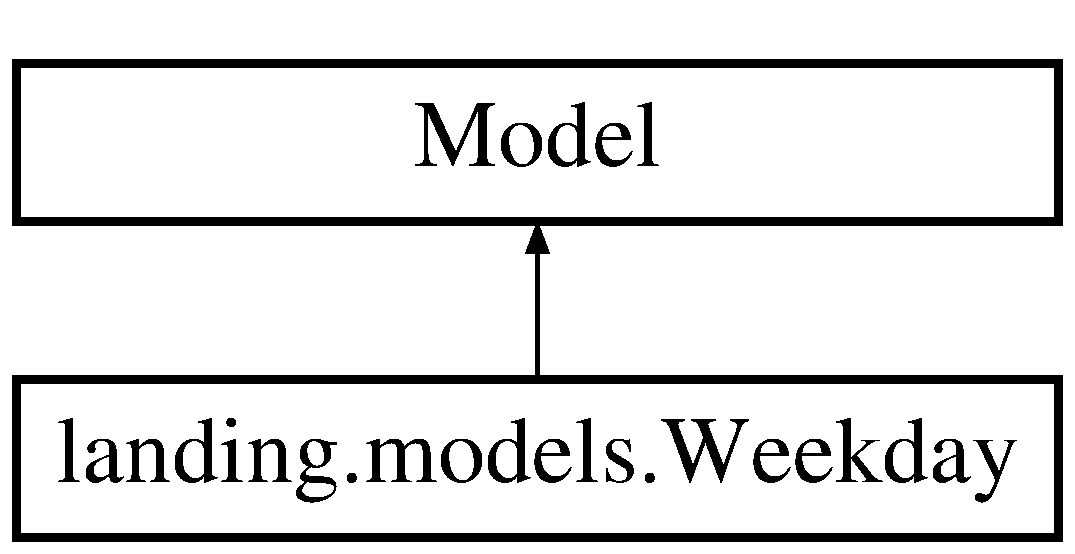
\includegraphics[height=2.000000cm]{classlanding_1_1models_1_1Weekday}
\end{center}
\end{figure}
\subsection*{Static Public Attributes}
\begin{DoxyCompactItemize}
\item 
tuple \mbox{\hyperlink{classlanding_1_1models_1_1Weekday_a7087116a99b548d0bfb99890d31b377a}{D\+A\+Y\+\_\+\+C\+H\+O\+I\+CE}}
\item 
string \mbox{\hyperlink{classlanding_1_1models_1_1Weekday_a7d9b7483659a0aa50e092bf758996cf1}{F}} = \char`\"{}Friday\char`\"{}
\item 
string \mbox{\hyperlink{classlanding_1_1models_1_1Weekday_ae349eee8108d59ddf4243538573aaaf4}{M}} = \char`\"{}Monday\char`\"{}
\item 
string \mbox{\hyperlink{classlanding_1_1models_1_1Weekday_ab05738a86ee9da4074c0b952a93e72e6}{R}} = \char`\"{}Thursday\char`\"{}
\item 
string \mbox{\hyperlink{classlanding_1_1models_1_1Weekday_afa57d936d921fb3d04172f0a7d690487}{S}} = \char`\"{}Saturday\char`\"{}
\item 
string \mbox{\hyperlink{classlanding_1_1models_1_1Weekday_ad441355f3f8b49c6de57ac0c0c90bd80}{T}} = \char`\"{}Tuesday\char`\"{}
\item 
string \mbox{\hyperlink{classlanding_1_1models_1_1Weekday_a2f5a7e4156f129c1dc20ff99bc71e72c}{U}} = \char`\"{}Sunday\char`\"{}
\item 
string \mbox{\hyperlink{classlanding_1_1models_1_1Weekday_a83e04a50723b1b692c2a0e0ca2e67068}{W}} = \char`\"{}Wednesday\char`\"{}
\item 
\mbox{\hyperlink{classlanding_1_1models_1_1Weekday_abf96c7b22336690bfb2fedd04a422ea2}{weekday\+\_\+name}} = models.\+Char\+Field(max\+\_\+length=10, choices=\mbox{\hyperlink{classlanding_1_1models_1_1Weekday_a7087116a99b548d0bfb99890d31b377a}{D\+A\+Y\+\_\+\+C\+H\+O\+I\+CE}}, default=None)
\end{DoxyCompactItemize}


\subsection{Detailed Description}
\begin{DoxyVerb}@Weekday holds what days classes are held, this includes the
        day of the week (i.e Monday, Wednesday). This helps students understand their schedule.
\end{DoxyVerb}
 

Definition at line 123 of file models.\+py.



\subsection{Member Data Documentation}
\mbox{\Hypertarget{classlanding_1_1models_1_1Weekday_a7087116a99b548d0bfb99890d31b377a}\label{classlanding_1_1models_1_1Weekday_a7087116a99b548d0bfb99890d31b377a}} 
\index{landing\+::models\+::\+Weekday@{landing\+::models\+::\+Weekday}!D\+A\+Y\+\_\+\+C\+H\+O\+I\+CE@{D\+A\+Y\+\_\+\+C\+H\+O\+I\+CE}}
\index{D\+A\+Y\+\_\+\+C\+H\+O\+I\+CE@{D\+A\+Y\+\_\+\+C\+H\+O\+I\+CE}!landing\+::models\+::\+Weekday@{landing\+::models\+::\+Weekday}}
\subsubsection{\texorpdfstring{D\+A\+Y\+\_\+\+C\+H\+O\+I\+CE}{DAY\_CHOICE}}
{\footnotesize\ttfamily tuple landing.\+models.\+Weekday.\+D\+A\+Y\+\_\+\+C\+H\+O\+I\+CE\hspace{0.3cm}{\ttfamily [static]}}

{\bfseries Initial value\+:}
\begin{DoxyCode}
=  (
        (M, \textcolor{stringliteral}{"Monday"}),
        (T, \textcolor{stringliteral}{"Tuesday"}),
        (W, \textcolor{stringliteral}{"Wednesday"}),
        (R, \textcolor{stringliteral}{"Thursday"}),
        (F, \textcolor{stringliteral}{"Friday"}),
        (S, \textcolor{stringliteral}{"Saturday"}),
        (U, \textcolor{stringliteral}{"Sunday"}),
    )
\end{DoxyCode}


Definition at line 135 of file models.\+py.

\mbox{\Hypertarget{classlanding_1_1models_1_1Weekday_a7d9b7483659a0aa50e092bf758996cf1}\label{classlanding_1_1models_1_1Weekday_a7d9b7483659a0aa50e092bf758996cf1}} 
\index{landing\+::models\+::\+Weekday@{landing\+::models\+::\+Weekday}!F@{F}}
\index{F@{F}!landing\+::models\+::\+Weekday@{landing\+::models\+::\+Weekday}}
\subsubsection{\texorpdfstring{F}{F}}
{\footnotesize\ttfamily string landing.\+models.\+Weekday.\+F = \char`\"{}Friday\char`\"{}\hspace{0.3cm}{\ttfamily [static]}}



Definition at line 132 of file models.\+py.

\mbox{\Hypertarget{classlanding_1_1models_1_1Weekday_ae349eee8108d59ddf4243538573aaaf4}\label{classlanding_1_1models_1_1Weekday_ae349eee8108d59ddf4243538573aaaf4}} 
\index{landing\+::models\+::\+Weekday@{landing\+::models\+::\+Weekday}!M@{M}}
\index{M@{M}!landing\+::models\+::\+Weekday@{landing\+::models\+::\+Weekday}}
\subsubsection{\texorpdfstring{M}{M}}
{\footnotesize\ttfamily string landing.\+models.\+Weekday.\+M = \char`\"{}Monday\char`\"{}\hspace{0.3cm}{\ttfamily [static]}}



Definition at line 128 of file models.\+py.

\mbox{\Hypertarget{classlanding_1_1models_1_1Weekday_ab05738a86ee9da4074c0b952a93e72e6}\label{classlanding_1_1models_1_1Weekday_ab05738a86ee9da4074c0b952a93e72e6}} 
\index{landing\+::models\+::\+Weekday@{landing\+::models\+::\+Weekday}!R@{R}}
\index{R@{R}!landing\+::models\+::\+Weekday@{landing\+::models\+::\+Weekday}}
\subsubsection{\texorpdfstring{R}{R}}
{\footnotesize\ttfamily string landing.\+models.\+Weekday.\+R = \char`\"{}Thursday\char`\"{}\hspace{0.3cm}{\ttfamily [static]}}



Definition at line 131 of file models.\+py.

\mbox{\Hypertarget{classlanding_1_1models_1_1Weekday_afa57d936d921fb3d04172f0a7d690487}\label{classlanding_1_1models_1_1Weekday_afa57d936d921fb3d04172f0a7d690487}} 
\index{landing\+::models\+::\+Weekday@{landing\+::models\+::\+Weekday}!S@{S}}
\index{S@{S}!landing\+::models\+::\+Weekday@{landing\+::models\+::\+Weekday}}
\subsubsection{\texorpdfstring{S}{S}}
{\footnotesize\ttfamily string landing.\+models.\+Weekday.\+S = \char`\"{}Saturday\char`\"{}\hspace{0.3cm}{\ttfamily [static]}}



Definition at line 133 of file models.\+py.

\mbox{\Hypertarget{classlanding_1_1models_1_1Weekday_ad441355f3f8b49c6de57ac0c0c90bd80}\label{classlanding_1_1models_1_1Weekday_ad441355f3f8b49c6de57ac0c0c90bd80}} 
\index{landing\+::models\+::\+Weekday@{landing\+::models\+::\+Weekday}!T@{T}}
\index{T@{T}!landing\+::models\+::\+Weekday@{landing\+::models\+::\+Weekday}}
\subsubsection{\texorpdfstring{T}{T}}
{\footnotesize\ttfamily string landing.\+models.\+Weekday.\+T = \char`\"{}Tuesday\char`\"{}\hspace{0.3cm}{\ttfamily [static]}}



Definition at line 129 of file models.\+py.

\mbox{\Hypertarget{classlanding_1_1models_1_1Weekday_a2f5a7e4156f129c1dc20ff99bc71e72c}\label{classlanding_1_1models_1_1Weekday_a2f5a7e4156f129c1dc20ff99bc71e72c}} 
\index{landing\+::models\+::\+Weekday@{landing\+::models\+::\+Weekday}!U@{U}}
\index{U@{U}!landing\+::models\+::\+Weekday@{landing\+::models\+::\+Weekday}}
\subsubsection{\texorpdfstring{U}{U}}
{\footnotesize\ttfamily string landing.\+models.\+Weekday.\+U = \char`\"{}Sunday\char`\"{}\hspace{0.3cm}{\ttfamily [static]}}



Definition at line 134 of file models.\+py.

\mbox{\Hypertarget{classlanding_1_1models_1_1Weekday_a83e04a50723b1b692c2a0e0ca2e67068}\label{classlanding_1_1models_1_1Weekday_a83e04a50723b1b692c2a0e0ca2e67068}} 
\index{landing\+::models\+::\+Weekday@{landing\+::models\+::\+Weekday}!W@{W}}
\index{W@{W}!landing\+::models\+::\+Weekday@{landing\+::models\+::\+Weekday}}
\subsubsection{\texorpdfstring{W}{W}}
{\footnotesize\ttfamily string landing.\+models.\+Weekday.\+W = \char`\"{}Wednesday\char`\"{}\hspace{0.3cm}{\ttfamily [static]}}



Definition at line 130 of file models.\+py.

\mbox{\Hypertarget{classlanding_1_1models_1_1Weekday_abf96c7b22336690bfb2fedd04a422ea2}\label{classlanding_1_1models_1_1Weekday_abf96c7b22336690bfb2fedd04a422ea2}} 
\index{landing\+::models\+::\+Weekday@{landing\+::models\+::\+Weekday}!weekday\+\_\+name@{weekday\+\_\+name}}
\index{weekday\+\_\+name@{weekday\+\_\+name}!landing\+::models\+::\+Weekday@{landing\+::models\+::\+Weekday}}
\subsubsection{\texorpdfstring{weekday\+\_\+name}{weekday\_name}}
{\footnotesize\ttfamily landing.\+models.\+Weekday.\+weekday\+\_\+name = models.\+Char\+Field(max\+\_\+length=10, choices=\mbox{\hyperlink{classlanding_1_1models_1_1Weekday_a7087116a99b548d0bfb99890d31b377a}{D\+A\+Y\+\_\+\+C\+H\+O\+I\+CE}}, default=None)\hspace{0.3cm}{\ttfamily [static]}}



Definition at line 144 of file models.\+py.



The documentation for this class was generated from the following file\+:\begin{DoxyCompactItemize}
\item 
mav\+Agenda/landing/\mbox{\hyperlink{models_8py}{models.\+py}}\end{DoxyCompactItemize}

\hypertarget{classlanding_1_1tests_1_1test__logic_1_1YourTestClass}{}\section{landing.\+tests.\+test\+\_\+logic.\+Your\+Test\+Class Class Reference}
\label{classlanding_1_1tests_1_1test__logic_1_1YourTestClass}\index{landing.\+tests.\+test\+\_\+logic.\+Your\+Test\+Class@{landing.\+tests.\+test\+\_\+logic.\+Your\+Test\+Class}}
Inheritance diagram for landing.\+tests.\+test\+\_\+logic.\+Your\+Test\+Class\+:\begin{figure}[H]
\begin{center}
\leavevmode
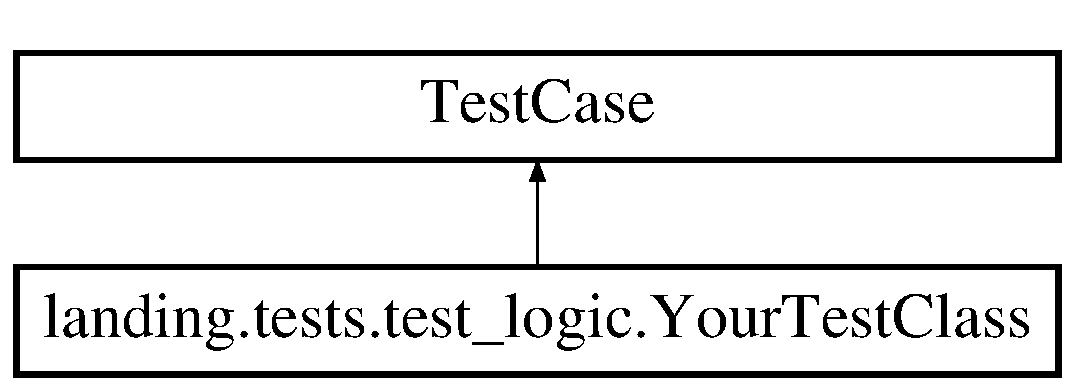
\includegraphics[height=2.000000cm]{classlanding_1_1tests_1_1test__logic_1_1YourTestClass}
\end{center}
\end{figure}
\subsection*{Public Member Functions}
\begin{DoxyCompactItemize}
\item 
def \mbox{\hyperlink{classlanding_1_1tests_1_1test__logic_1_1YourTestClass_a8fc08e836ba1d71ef27e4fb442f9bf07}{set\+Up}} (self)
\item 
def \mbox{\hyperlink{classlanding_1_1tests_1_1test__logic_1_1YourTestClass_aa5874621de0a637a917adb181465565b}{tear\+Down}} (self)
\item 
def \mbox{\hyperlink{classlanding_1_1tests_1_1test__logic_1_1YourTestClass_ad3383bb3b183fd5da69ed5af9ebf895f}{test\+\_\+email\+Found}} (self)
\item 
def \mbox{\hyperlink{classlanding_1_1tests_1_1test__logic_1_1YourTestClass_a217df4c55c33a905e5a8acedbabc2554}{test\+\_\+generate\+\_\+new\+\_\+semester}} (self)
\item 
def \mbox{\hyperlink{classlanding_1_1tests_1_1test__logic_1_1YourTestClass_a299e310958f4c2310742a166666ce54a}{test\+\_\+generate\+Concentrations\+DD}} (self)
\item 
def \mbox{\hyperlink{classlanding_1_1tests_1_1test__logic_1_1YourTestClass_a3bd96c391d99f1099fdd3145ec8bb244}{test\+\_\+generate\+Diploma\+DD}} (self)
\item 
def \mbox{\hyperlink{classlanding_1_1tests_1_1test__logic_1_1YourTestClass_a07dc170a7378ab65e26198097bf79421}{test\+\_\+generate\+Major\+DD}} (self)
\item 
def \mbox{\hyperlink{classlanding_1_1tests_1_1test__logic_1_1YourTestClass_a4ef706cd4dd8262484f5e25f04e5f673}{test\+\_\+generate\+Minor\+DD}} (self)
\item 
def \mbox{\hyperlink{classlanding_1_1tests_1_1test__logic_1_1YourTestClass_a7ccbc5812985183c73be2a72de119497}{test\+\_\+get\+\_\+semester\+\_\+by\+\_\+month\+\_\+year}} (self)
\item 
def \mbox{\hyperlink{classlanding_1_1tests_1_1test__logic_1_1YourTestClass_a9e136af10d0f563ebb4a3a1b1075a6ed}{test\+\_\+get\+Degree}} (self)
\item 
def \mbox{\hyperlink{classlanding_1_1tests_1_1test__logic_1_1YourTestClass_a052a9215642dc369fea184e2e6882b91}{test\+\_\+get\+User\+By\+Email}} (self)
\item 
def \mbox{\hyperlink{classlanding_1_1tests_1_1test__logic_1_1YourTestClass_a27205d7c768e925bf201ff242d7c6137}{test\+\_\+is\+\_\+full}} (self)
\item 
def \mbox{\hyperlink{classlanding_1_1tests_1_1test__logic_1_1YourTestClass_ac0dd592f4aa2af5461ed9e4622e6ff10}{test\+\_\+remove\+Courses\+Taken}} (self)
\end{DoxyCompactItemize}


\subsection{Detailed Description}


Definition at line 10 of file test\+\_\+logic.\+py.



\subsection{Member Function Documentation}
\mbox{\Hypertarget{classlanding_1_1tests_1_1test__logic_1_1YourTestClass_a8fc08e836ba1d71ef27e4fb442f9bf07}\label{classlanding_1_1tests_1_1test__logic_1_1YourTestClass_a8fc08e836ba1d71ef27e4fb442f9bf07}} 
\index{landing\+::tests\+::test\+\_\+logic\+::\+Your\+Test\+Class@{landing\+::tests\+::test\+\_\+logic\+::\+Your\+Test\+Class}!set\+Up@{set\+Up}}
\index{set\+Up@{set\+Up}!landing\+::tests\+::test\+\_\+logic\+::\+Your\+Test\+Class@{landing\+::tests\+::test\+\_\+logic\+::\+Your\+Test\+Class}}
\subsubsection{\texorpdfstring{set\+Up()}{setUp()}}
{\footnotesize\ttfamily def landing.\+tests.\+test\+\_\+logic.\+Your\+Test\+Class.\+set\+Up (\begin{DoxyParamCaption}\item[{}]{self }\end{DoxyParamCaption})}



Definition at line 12 of file test\+\_\+logic.\+py.

\mbox{\Hypertarget{classlanding_1_1tests_1_1test__logic_1_1YourTestClass_aa5874621de0a637a917adb181465565b}\label{classlanding_1_1tests_1_1test__logic_1_1YourTestClass_aa5874621de0a637a917adb181465565b}} 
\index{landing\+::tests\+::test\+\_\+logic\+::\+Your\+Test\+Class@{landing\+::tests\+::test\+\_\+logic\+::\+Your\+Test\+Class}!tear\+Down@{tear\+Down}}
\index{tear\+Down@{tear\+Down}!landing\+::tests\+::test\+\_\+logic\+::\+Your\+Test\+Class@{landing\+::tests\+::test\+\_\+logic\+::\+Your\+Test\+Class}}
\subsubsection{\texorpdfstring{tear\+Down()}{tearDown()}}
{\footnotesize\ttfamily def landing.\+tests.\+test\+\_\+logic.\+Your\+Test\+Class.\+tear\+Down (\begin{DoxyParamCaption}\item[{}]{self }\end{DoxyParamCaption})}



Definition at line 16 of file test\+\_\+logic.\+py.

\mbox{\Hypertarget{classlanding_1_1tests_1_1test__logic_1_1YourTestClass_ad3383bb3b183fd5da69ed5af9ebf895f}\label{classlanding_1_1tests_1_1test__logic_1_1YourTestClass_ad3383bb3b183fd5da69ed5af9ebf895f}} 
\index{landing\+::tests\+::test\+\_\+logic\+::\+Your\+Test\+Class@{landing\+::tests\+::test\+\_\+logic\+::\+Your\+Test\+Class}!test\+\_\+email\+Found@{test\+\_\+email\+Found}}
\index{test\+\_\+email\+Found@{test\+\_\+email\+Found}!landing\+::tests\+::test\+\_\+logic\+::\+Your\+Test\+Class@{landing\+::tests\+::test\+\_\+logic\+::\+Your\+Test\+Class}}
\subsubsection{\texorpdfstring{test\+\_\+email\+Found()}{test\_emailFound()}}
{\footnotesize\ttfamily def landing.\+tests.\+test\+\_\+logic.\+Your\+Test\+Class.\+test\+\_\+email\+Found (\begin{DoxyParamCaption}\item[{}]{self }\end{DoxyParamCaption})}

\begin{DoxyVerb}@test_emailFound stores a user into the database and checks that the email is found in the database
@param self references current instance of the class
\end{DoxyVerb}
 

Definition at line 478 of file test\+\_\+logic.\+py.



References landing.\+views.\+email\+Found().

\mbox{\Hypertarget{classlanding_1_1tests_1_1test__logic_1_1YourTestClass_a217df4c55c33a905e5a8acedbabc2554}\label{classlanding_1_1tests_1_1test__logic_1_1YourTestClass_a217df4c55c33a905e5a8acedbabc2554}} 
\index{landing\+::tests\+::test\+\_\+logic\+::\+Your\+Test\+Class@{landing\+::tests\+::test\+\_\+logic\+::\+Your\+Test\+Class}!test\+\_\+generate\+\_\+new\+\_\+semester@{test\+\_\+generate\+\_\+new\+\_\+semester}}
\index{test\+\_\+generate\+\_\+new\+\_\+semester@{test\+\_\+generate\+\_\+new\+\_\+semester}!landing\+::tests\+::test\+\_\+logic\+::\+Your\+Test\+Class@{landing\+::tests\+::test\+\_\+logic\+::\+Your\+Test\+Class}}
\subsubsection{\texorpdfstring{test\+\_\+generate\+\_\+new\+\_\+semester()}{test\_generate\_new\_semester()}}
{\footnotesize\ttfamily def landing.\+tests.\+test\+\_\+logic.\+Your\+Test\+Class.\+test\+\_\+generate\+\_\+new\+\_\+semester (\begin{DoxyParamCaption}\item[{}]{self }\end{DoxyParamCaption})}

\begin{DoxyVerb}@test_generate_new_semester tests if a semester is created and stored correctly
@param self references current instance of the class
\end{DoxyVerb}
 

Definition at line 360 of file test\+\_\+logic.\+py.



References landing.\+views.\+generate\+New\+Semester(), and landing.\+views.\+get\+Semester\+By\+Month\+Year().

\mbox{\Hypertarget{classlanding_1_1tests_1_1test__logic_1_1YourTestClass_a299e310958f4c2310742a166666ce54a}\label{classlanding_1_1tests_1_1test__logic_1_1YourTestClass_a299e310958f4c2310742a166666ce54a}} 
\index{landing\+::tests\+::test\+\_\+logic\+::\+Your\+Test\+Class@{landing\+::tests\+::test\+\_\+logic\+::\+Your\+Test\+Class}!test\+\_\+generate\+Concentrations\+DD@{test\+\_\+generate\+Concentrations\+DD}}
\index{test\+\_\+generate\+Concentrations\+DD@{test\+\_\+generate\+Concentrations\+DD}!landing\+::tests\+::test\+\_\+logic\+::\+Your\+Test\+Class@{landing\+::tests\+::test\+\_\+logic\+::\+Your\+Test\+Class}}
\subsubsection{\texorpdfstring{test\+\_\+generate\+Concentrations\+D\+D()}{test\_generateConcentrationsDD()}}
{\footnotesize\ttfamily def landing.\+tests.\+test\+\_\+logic.\+Your\+Test\+Class.\+test\+\_\+generate\+Concentrations\+DD (\begin{DoxyParamCaption}\item[{}]{self }\end{DoxyParamCaption})}

\begin{DoxyVerb}@test_generateConcentrationsDD creates a list of possible concentrations for use on the createuser page
@param self references current instance of the class
\end{DoxyVerb}
 

Definition at line 448 of file test\+\_\+logic.\+py.



References landing.\+views.\+generate\+Concentrations\+D\+D().

\mbox{\Hypertarget{classlanding_1_1tests_1_1test__logic_1_1YourTestClass_a3bd96c391d99f1099fdd3145ec8bb244}\label{classlanding_1_1tests_1_1test__logic_1_1YourTestClass_a3bd96c391d99f1099fdd3145ec8bb244}} 
\index{landing\+::tests\+::test\+\_\+logic\+::\+Your\+Test\+Class@{landing\+::tests\+::test\+\_\+logic\+::\+Your\+Test\+Class}!test\+\_\+generate\+Diploma\+DD@{test\+\_\+generate\+Diploma\+DD}}
\index{test\+\_\+generate\+Diploma\+DD@{test\+\_\+generate\+Diploma\+DD}!landing\+::tests\+::test\+\_\+logic\+::\+Your\+Test\+Class@{landing\+::tests\+::test\+\_\+logic\+::\+Your\+Test\+Class}}
\subsubsection{\texorpdfstring{test\+\_\+generate\+Diploma\+D\+D()}{test\_generateDiplomaDD()}}
{\footnotesize\ttfamily def landing.\+tests.\+test\+\_\+logic.\+Your\+Test\+Class.\+test\+\_\+generate\+Diploma\+DD (\begin{DoxyParamCaption}\item[{}]{self }\end{DoxyParamCaption})}

\begin{DoxyVerb}@test_generateDiplomaDD creates a list of possible diplomas for use on the createuser page
@param self references current instance of the class
\end{DoxyVerb}
 

Definition at line 461 of file test\+\_\+logic.\+py.



References landing.\+views.\+generate\+Diploma\+D\+D().

\mbox{\Hypertarget{classlanding_1_1tests_1_1test__logic_1_1YourTestClass_a07dc170a7378ab65e26198097bf79421}\label{classlanding_1_1tests_1_1test__logic_1_1YourTestClass_a07dc170a7378ab65e26198097bf79421}} 
\index{landing\+::tests\+::test\+\_\+logic\+::\+Your\+Test\+Class@{landing\+::tests\+::test\+\_\+logic\+::\+Your\+Test\+Class}!test\+\_\+generate\+Major\+DD@{test\+\_\+generate\+Major\+DD}}
\index{test\+\_\+generate\+Major\+DD@{test\+\_\+generate\+Major\+DD}!landing\+::tests\+::test\+\_\+logic\+::\+Your\+Test\+Class@{landing\+::tests\+::test\+\_\+logic\+::\+Your\+Test\+Class}}
\subsubsection{\texorpdfstring{test\+\_\+generate\+Major\+D\+D()}{test\_generateMajorDD()}}
{\footnotesize\ttfamily def landing.\+tests.\+test\+\_\+logic.\+Your\+Test\+Class.\+test\+\_\+generate\+Major\+DD (\begin{DoxyParamCaption}\item[{}]{self }\end{DoxyParamCaption})}

\begin{DoxyVerb}@test_generateMajorDD creates a list of possible majors for use on the createuser page
@param self references current instance of the class
\end{DoxyVerb}
 

Definition at line 414 of file test\+\_\+logic.\+py.



References landing.\+views.\+generate\+Major\+D\+D().

\mbox{\Hypertarget{classlanding_1_1tests_1_1test__logic_1_1YourTestClass_a4ef706cd4dd8262484f5e25f04e5f673}\label{classlanding_1_1tests_1_1test__logic_1_1YourTestClass_a4ef706cd4dd8262484f5e25f04e5f673}} 
\index{landing\+::tests\+::test\+\_\+logic\+::\+Your\+Test\+Class@{landing\+::tests\+::test\+\_\+logic\+::\+Your\+Test\+Class}!test\+\_\+generate\+Minor\+DD@{test\+\_\+generate\+Minor\+DD}}
\index{test\+\_\+generate\+Minor\+DD@{test\+\_\+generate\+Minor\+DD}!landing\+::tests\+::test\+\_\+logic\+::\+Your\+Test\+Class@{landing\+::tests\+::test\+\_\+logic\+::\+Your\+Test\+Class}}
\subsubsection{\texorpdfstring{test\+\_\+generate\+Minor\+D\+D()}{test\_generateMinorDD()}}
{\footnotesize\ttfamily def landing.\+tests.\+test\+\_\+logic.\+Your\+Test\+Class.\+test\+\_\+generate\+Minor\+DD (\begin{DoxyParamCaption}\item[{}]{self }\end{DoxyParamCaption})}

\begin{DoxyVerb}@test_generateMinorDD creates a list of possible minors for use on the createuser page
@param self references current instance of the class
\end{DoxyVerb}
 

Definition at line 434 of file test\+\_\+logic.\+py.



References landing.\+views.\+generate\+Minor\+D\+D().

\mbox{\Hypertarget{classlanding_1_1tests_1_1test__logic_1_1YourTestClass_a7ccbc5812985183c73be2a72de119497}\label{classlanding_1_1tests_1_1test__logic_1_1YourTestClass_a7ccbc5812985183c73be2a72de119497}} 
\index{landing\+::tests\+::test\+\_\+logic\+::\+Your\+Test\+Class@{landing\+::tests\+::test\+\_\+logic\+::\+Your\+Test\+Class}!test\+\_\+get\+\_\+semester\+\_\+by\+\_\+month\+\_\+year@{test\+\_\+get\+\_\+semester\+\_\+by\+\_\+month\+\_\+year}}
\index{test\+\_\+get\+\_\+semester\+\_\+by\+\_\+month\+\_\+year@{test\+\_\+get\+\_\+semester\+\_\+by\+\_\+month\+\_\+year}!landing\+::tests\+::test\+\_\+logic\+::\+Your\+Test\+Class@{landing\+::tests\+::test\+\_\+logic\+::\+Your\+Test\+Class}}
\subsubsection{\texorpdfstring{test\+\_\+get\+\_\+semester\+\_\+by\+\_\+month\+\_\+year()}{test\_get\_semester\_by\_month\_year()}}
{\footnotesize\ttfamily def landing.\+tests.\+test\+\_\+logic.\+Your\+Test\+Class.\+test\+\_\+get\+\_\+semester\+\_\+by\+\_\+month\+\_\+year (\begin{DoxyParamCaption}\item[{}]{self }\end{DoxyParamCaption})}

\begin{DoxyVerb}@test_get_semester_by_month_year tests if the correct semester is calculated
@param self references current instance of the class
\end{DoxyVerb}
 

Definition at line 343 of file test\+\_\+logic.\+py.



References landing.\+views.\+get\+Semester\+By\+Month\+Year().

\mbox{\Hypertarget{classlanding_1_1tests_1_1test__logic_1_1YourTestClass_a9e136af10d0f563ebb4a3a1b1075a6ed}\label{classlanding_1_1tests_1_1test__logic_1_1YourTestClass_a9e136af10d0f563ebb4a3a1b1075a6ed}} 
\index{landing\+::tests\+::test\+\_\+logic\+::\+Your\+Test\+Class@{landing\+::tests\+::test\+\_\+logic\+::\+Your\+Test\+Class}!test\+\_\+get\+Degree@{test\+\_\+get\+Degree}}
\index{test\+\_\+get\+Degree@{test\+\_\+get\+Degree}!landing\+::tests\+::test\+\_\+logic\+::\+Your\+Test\+Class@{landing\+::tests\+::test\+\_\+logic\+::\+Your\+Test\+Class}}
\subsubsection{\texorpdfstring{test\+\_\+get\+Degree()}{test\_getDegree()}}
{\footnotesize\ttfamily def landing.\+tests.\+test\+\_\+logic.\+Your\+Test\+Class.\+test\+\_\+get\+Degree (\begin{DoxyParamCaption}\item[{}]{self }\end{DoxyParamCaption})}

\begin{DoxyVerb}@test_getDegree creates a degree object and checks that the degree is stored in the SQLite3 database
@param self references current instance of the class
\end{DoxyVerb}
 

Definition at line 215 of file test\+\_\+logic.\+py.



References landing.\+views.\+get\+Degree().

\mbox{\Hypertarget{classlanding_1_1tests_1_1test__logic_1_1YourTestClass_a052a9215642dc369fea184e2e6882b91}\label{classlanding_1_1tests_1_1test__logic_1_1YourTestClass_a052a9215642dc369fea184e2e6882b91}} 
\index{landing\+::tests\+::test\+\_\+logic\+::\+Your\+Test\+Class@{landing\+::tests\+::test\+\_\+logic\+::\+Your\+Test\+Class}!test\+\_\+get\+User\+By\+Email@{test\+\_\+get\+User\+By\+Email}}
\index{test\+\_\+get\+User\+By\+Email@{test\+\_\+get\+User\+By\+Email}!landing\+::tests\+::test\+\_\+logic\+::\+Your\+Test\+Class@{landing\+::tests\+::test\+\_\+logic\+::\+Your\+Test\+Class}}
\subsubsection{\texorpdfstring{test\+\_\+get\+User\+By\+Email()}{test\_getUserByEmail()}}
{\footnotesize\ttfamily def landing.\+tests.\+test\+\_\+logic.\+Your\+Test\+Class.\+test\+\_\+get\+User\+By\+Email (\begin{DoxyParamCaption}\item[{}]{self }\end{DoxyParamCaption})}

\begin{DoxyVerb}    @test_getUserByEmail creates a user account and checks that the account is stored in the SQLite3 database
    @param self references current instance of the class
    @var email sample username string to store in SQLite3 database
    @var p  sample password string to store in SQLite3 database\end{DoxyVerb}
 

Definition at line 195 of file test\+\_\+logic.\+py.



References landing.\+views.\+get\+User\+By\+Email().

\mbox{\Hypertarget{classlanding_1_1tests_1_1test__logic_1_1YourTestClass_a27205d7c768e925bf201ff242d7c6137}\label{classlanding_1_1tests_1_1test__logic_1_1YourTestClass_a27205d7c768e925bf201ff242d7c6137}} 
\index{landing\+::tests\+::test\+\_\+logic\+::\+Your\+Test\+Class@{landing\+::tests\+::test\+\_\+logic\+::\+Your\+Test\+Class}!test\+\_\+is\+\_\+full@{test\+\_\+is\+\_\+full}}
\index{test\+\_\+is\+\_\+full@{test\+\_\+is\+\_\+full}!landing\+::tests\+::test\+\_\+logic\+::\+Your\+Test\+Class@{landing\+::tests\+::test\+\_\+logic\+::\+Your\+Test\+Class}}
\subsubsection{\texorpdfstring{test\+\_\+is\+\_\+full()}{test\_is\_full()}}
{\footnotesize\ttfamily def landing.\+tests.\+test\+\_\+logic.\+Your\+Test\+Class.\+test\+\_\+is\+\_\+full (\begin{DoxyParamCaption}\item[{}]{self }\end{DoxyParamCaption})}

\begin{DoxyVerb}@test_is_full tests if the semester has hit the maximum number of credits allowable
@param self references current instance of the class
\end{DoxyVerb}
 

Definition at line 379 of file test\+\_\+logic.\+py.



References landing.\+views.\+generate\+New\+Semester(), landing.\+views.\+get\+Semester\+By\+Month\+Year(), and landing.\+views.\+is\+Full().

\mbox{\Hypertarget{classlanding_1_1tests_1_1test__logic_1_1YourTestClass_ac0dd592f4aa2af5461ed9e4622e6ff10}\label{classlanding_1_1tests_1_1test__logic_1_1YourTestClass_ac0dd592f4aa2af5461ed9e4622e6ff10}} 
\index{landing\+::tests\+::test\+\_\+logic\+::\+Your\+Test\+Class@{landing\+::tests\+::test\+\_\+logic\+::\+Your\+Test\+Class}!test\+\_\+remove\+Courses\+Taken@{test\+\_\+remove\+Courses\+Taken}}
\index{test\+\_\+remove\+Courses\+Taken@{test\+\_\+remove\+Courses\+Taken}!landing\+::tests\+::test\+\_\+logic\+::\+Your\+Test\+Class@{landing\+::tests\+::test\+\_\+logic\+::\+Your\+Test\+Class}}
\subsubsection{\texorpdfstring{test\+\_\+remove\+Courses\+Taken()}{test\_removeCoursesTaken()}}
{\footnotesize\ttfamily def landing.\+tests.\+test\+\_\+logic.\+Your\+Test\+Class.\+test\+\_\+remove\+Courses\+Taken (\begin{DoxyParamCaption}\item[{}]{self }\end{DoxyParamCaption})}

\begin{DoxyVerb}@test_removeCoursesTaken tests the correctness of the computed list of classes a user still needs to take in order to graduate
@param self references current instance of the class
\end{DoxyVerb}
 

Definition at line 271 of file test\+\_\+logic.\+py.



References landing.\+views.\+remove\+Courses\+Taken().



The documentation for this class was generated from the following file\+:\begin{DoxyCompactItemize}
\item 
mav\+Agenda/landing/tests/\mbox{\hyperlink{test__logic_8py}{test\+\_\+logic.\+py}}\end{DoxyCompactItemize}

\chapter{File Documentation}
\hypertarget{scrape_8py}{}\section{C\+:/\+Users/lauren/\+Pycharm\+Projects/\+Mav\+Link\+Made\+Easy/matriculation\+Utility/scrape.py File Reference}
\label{scrape_8py}\index{C\+:/\+Users/lauren/\+Pycharm\+Projects/\+Mav\+Link\+Made\+Easy/matriculation\+Utility/scrape.\+py@{C\+:/\+Users/lauren/\+Pycharm\+Projects/\+Mav\+Link\+Made\+Easy/matriculation\+Utility/scrape.\+py}}
\subsection*{Namespaces}
\begin{DoxyCompactItemize}
\item 
 \mbox{\hyperlink{namespacescrape}{scrape}}
\end{DoxyCompactItemize}
\subsection*{Functions}
\begin{DoxyCompactItemize}
\item 
def \mbox{\hyperlink{namespacescrape_ac72ffc4d789a94d65b548726045faa93}{scrape.\+add\+Req\+Section}} (title, dept, num, desc, xx)
\item 
def \mbox{\hyperlink{namespacescrape_a5653dd5601f9b92af6a260a7fab1ff43}{scrape.\+main}} ()
\end{DoxyCompactItemize}

\hypertarget{landing_2____init_____8py}{}\section{mav\+Agenda/landing/\+\_\+\+\_\+init\+\_\+\+\_\+.py File Reference}
\label{landing_2____init_____8py}\index{mav\+Agenda/landing/\+\_\+\+\_\+init\+\_\+\+\_\+.\+py@{mav\+Agenda/landing/\+\_\+\+\_\+init\+\_\+\+\_\+.\+py}}
\subsection*{Namespaces}
\begin{DoxyCompactItemize}
\item 
 \mbox{\hyperlink{namespacelanding}{landing}}
\end{DoxyCompactItemize}

\hypertarget{landing_2migrations_2____init_____8py}{}\section{C\+:/\+Users/lauren/\+Pycharm\+Projects/\+Mav\+Link\+Made\+Easy/mav\+Agenda/landing/migrations/\+\_\+\+\_\+init\+\_\+\+\_\+.py File Reference}
\label{landing_2migrations_2____init_____8py}\index{C\+:/\+Users/lauren/\+Pycharm\+Projects/\+Mav\+Link\+Made\+Easy/mav\+Agenda/landing/migrations/\+\_\+\+\_\+init\+\_\+\+\_\+.\+py@{C\+:/\+Users/lauren/\+Pycharm\+Projects/\+Mav\+Link\+Made\+Easy/mav\+Agenda/landing/migrations/\+\_\+\+\_\+init\+\_\+\+\_\+.\+py}}
\subsection*{Namespaces}
\begin{DoxyCompactItemize}
\item 
 \mbox{\hyperlink{namespacemavAgenda_1_1landing_1_1migrations}{mav\+Agenda.\+landing.\+migrations}}
\end{DoxyCompactItemize}

\hypertarget{landing_2tests_2____init_____8py}{}\section{mav\+Agenda/landing/tests/\+\_\+\+\_\+init\+\_\+\+\_\+.py File Reference}
\label{landing_2tests_2____init_____8py}\index{mav\+Agenda/landing/tests/\+\_\+\+\_\+init\+\_\+\+\_\+.\+py@{mav\+Agenda/landing/tests/\+\_\+\+\_\+init\+\_\+\+\_\+.\+py}}
\subsection*{Namespaces}
\begin{DoxyCompactItemize}
\item 
 \mbox{\hyperlink{namespacelanding_1_1tests}{landing.\+tests}}
\end{DoxyCompactItemize}

\hypertarget{mavAgenda_2____init_____8py}{}\section{mav\+Agenda/mav\+Agenda/\+\_\+\+\_\+init\+\_\+\+\_\+.py File Reference}
\label{mavAgenda_2____init_____8py}\index{mav\+Agenda/mav\+Agenda/\+\_\+\+\_\+init\+\_\+\+\_\+.\+py@{mav\+Agenda/mav\+Agenda/\+\_\+\+\_\+init\+\_\+\+\_\+.\+py}}
\subsection*{Namespaces}
\begin{DoxyCompactItemize}
\item 
 \mbox{\hyperlink{namespacemavAgenda}{mav\+Agenda}}
\end{DoxyCompactItemize}

\hypertarget{templates_2____init_____8py}{}\section{C\+:/\+Users/lauren/\+Pycharm\+Projects/\+Mav\+Link\+Made\+Easy/mav\+Agenda/templates/\+\_\+\+\_\+init\+\_\+\+\_\+.py File Reference}
\label{templates_2____init_____8py}\index{C\+:/\+Users/lauren/\+Pycharm\+Projects/\+Mav\+Link\+Made\+Easy/mav\+Agenda/templates/\+\_\+\+\_\+init\+\_\+\+\_\+.\+py@{C\+:/\+Users/lauren/\+Pycharm\+Projects/\+Mav\+Link\+Made\+Easy/mav\+Agenda/templates/\+\_\+\+\_\+init\+\_\+\+\_\+.\+py}}
\subsection*{Namespaces}
\begin{DoxyCompactItemize}
\item 
 \mbox{\hyperlink{namespacemavAgenda_1_1templates}{mav\+Agenda.\+templates}}
\end{DoxyCompactItemize}

\hypertarget{admin_8py}{}\section{mav\+Agenda/landing/admin.py File Reference}
\label{admin_8py}\index{mav\+Agenda/landing/admin.\+py@{mav\+Agenda/landing/admin.\+py}}
\subsection*{Namespaces}
\begin{DoxyCompactItemize}
\item 
 \mbox{\hyperlink{namespacelanding_1_1admin}{landing.\+admin}}
\end{DoxyCompactItemize}

\hypertarget{apps_8py}{}\section{mav\+Agenda/landing/apps.py File Reference}
\label{apps_8py}\index{mav\+Agenda/landing/apps.\+py@{mav\+Agenda/landing/apps.\+py}}
\subsection*{Classes}
\begin{DoxyCompactItemize}
\item 
class \mbox{\hyperlink{classlanding_1_1apps_1_1LandingConfig}{landing.\+apps.\+Landing\+Config}}
\end{DoxyCompactItemize}
\subsection*{Namespaces}
\begin{DoxyCompactItemize}
\item 
 \mbox{\hyperlink{namespacelanding_1_1apps}{landing.\+apps}}
\end{DoxyCompactItemize}

\hypertarget{forms_8py}{}\section{mav\+Agenda/landing/forms.py File Reference}
\label{forms_8py}\index{mav\+Agenda/landing/forms.\+py@{mav\+Agenda/landing/forms.\+py}}
\subsection*{Classes}
\begin{DoxyCompactItemize}
\item 
class \mbox{\hyperlink{classlanding_1_1forms_1_1UserForm_1_1Meta}{landing.\+forms.\+User\+Form.\+Meta}}
\item 
class \mbox{\hyperlink{classlanding_1_1forms_1_1UserForm}{landing.\+forms.\+User\+Form}}
\end{DoxyCompactItemize}
\subsection*{Namespaces}
\begin{DoxyCompactItemize}
\item 
 \mbox{\hyperlink{namespacelanding_1_1forms}{landing.\+forms}}
\end{DoxyCompactItemize}

\hypertarget{0001__initial_8py}{}\section{mav\+Agenda/landing/migrations/0001\+\_\+initial.py File Reference}
\label{0001__initial_8py}\index{mav\+Agenda/landing/migrations/0001\+\_\+initial.\+py@{mav\+Agenda/landing/migrations/0001\+\_\+initial.\+py}}
\subsection*{Classes}
\begin{DoxyCompactItemize}
\item 
class \mbox{\hyperlink{classlanding_1_1migrations_1_10001__initial_1_1Migration}{landing.\+migrations.\+0001\+\_\+initial.\+Migration}}
\end{DoxyCompactItemize}
\subsection*{Namespaces}
\begin{DoxyCompactItemize}
\item 
 \mbox{\hyperlink{namespacelanding_1_1migrations_1_10001__initial}{landing.\+migrations.\+0001\+\_\+initial}}
\end{DoxyCompactItemize}

\hypertarget{models_8py}{}\section{mav\+Agenda/landing/models.py File Reference}
\label{models_8py}\index{mav\+Agenda/landing/models.\+py@{mav\+Agenda/landing/models.\+py}}
\subsection*{Classes}
\begin{DoxyCompactItemize}
\item 
class \mbox{\hyperlink{classlanding_1_1models_1_1Building}{landing.\+models.\+Building}}
\item 
class \mbox{\hyperlink{classlanding_1_1models_1_1Campus}{landing.\+models.\+Campus}}
\item 
class \mbox{\hyperlink{classlanding_1_1models_1_1Complete}{landing.\+models.\+Complete}}
\item 
class \mbox{\hyperlink{classlanding_1_1models_1_1Course}{landing.\+models.\+Course}}
\item 
class \mbox{\hyperlink{classlanding_1_1models_1_1Degree}{landing.\+models.\+Degree}}
\item 
class \mbox{\hyperlink{classlanding_1_1models_1_1Instructor}{landing.\+models.\+Instructor}}
\item 
class \mbox{\hyperlink{classlanding_1_1models_1_1Offering}{landing.\+models.\+Offering}}
\item 
class \mbox{\hyperlink{classlanding_1_1models_1_1Prereq}{landing.\+models.\+Prereq}}
\item 
class \mbox{\hyperlink{classlanding_1_1models_1_1Requirement}{landing.\+models.\+Requirement}}
\item 
class \mbox{\hyperlink{classlanding_1_1models_1_1UserPreferences}{landing.\+models.\+User\+Preferences}}
\item 
class \mbox{\hyperlink{classlanding_1_1models_1_1Weekday}{landing.\+models.\+Weekday}}
\end{DoxyCompactItemize}
\subsection*{Namespaces}
\begin{DoxyCompactItemize}
\item 
 \mbox{\hyperlink{namespacelanding_1_1models}{landing.\+models}}
\end{DoxyCompactItemize}

\hypertarget{base_8html}{}\section{C\+:/\+Users/lauren/\+Pycharm\+Projects/\+Mav\+Link\+Made\+Easy/mav\+Agenda/landing/templates/landing/base.html File Reference}
\label{base_8html}\index{C\+:/\+Users/lauren/\+Pycharm\+Projects/\+Mav\+Link\+Made\+Easy/mav\+Agenda/landing/templates/landing/base.\+html@{C\+:/\+Users/lauren/\+Pycharm\+Projects/\+Mav\+Link\+Made\+Easy/mav\+Agenda/landing/templates/landing/base.\+html}}

\hypertarget{createuser_8html}{}\section{mav\+Agenda/landing/templates/landing/createuser.html File Reference}
\label{createuser_8html}\index{mav\+Agenda/landing/templates/landing/createuser.\+html@{mav\+Agenda/landing/templates/landing/createuser.\+html}}

\hypertarget{login_8html}{}\section{C\+:/\+Users/lauren/\+Pycharm\+Projects/\+Mav\+Link\+Made\+Easy/mav\+Agenda/landing/templates/landing/login.html File Reference}
\label{login_8html}\index{C\+:/\+Users/lauren/\+Pycharm\+Projects/\+Mav\+Link\+Made\+Easy/mav\+Agenda/landing/templates/landing/login.\+html@{C\+:/\+Users/lauren/\+Pycharm\+Projects/\+Mav\+Link\+Made\+Easy/mav\+Agenda/landing/templates/landing/login.\+html}}

\hypertarget{nextsemesterpreferences_8html}{}\section{C\+:/\+Users/lauren/\+Pycharm\+Projects/\+Mav\+Link\+Made\+Easy/mav\+Agenda/landing/templates/landing/nextsemesterpreferences.html File Reference}
\label{nextsemesterpreferences_8html}\index{C\+:/\+Users/lauren/\+Pycharm\+Projects/\+Mav\+Link\+Made\+Easy/mav\+Agenda/landing/templates/landing/nextsemesterpreferences.\+html@{C\+:/\+Users/lauren/\+Pycharm\+Projects/\+Mav\+Link\+Made\+Easy/mav\+Agenda/landing/templates/landing/nextsemesterpreferences.\+html}}

\hypertarget{schedule_8html}{}\section{C\+:/\+Users/lauren/\+Pycharm\+Projects/\+Mav\+Link\+Made\+Easy/mav\+Agenda/landing/templates/landing/schedule.html File Reference}
\label{schedule_8html}\index{C\+:/\+Users/lauren/\+Pycharm\+Projects/\+Mav\+Link\+Made\+Easy/mav\+Agenda/landing/templates/landing/schedule.\+html@{C\+:/\+Users/lauren/\+Pycharm\+Projects/\+Mav\+Link\+Made\+Easy/mav\+Agenda/landing/templates/landing/schedule.\+html}}

\hypertarget{selectcourses_8html}{}\section{C\+:/\+Users/lauren/\+Pycharm\+Projects/\+Mav\+Link\+Made\+Easy/mav\+Agenda/landing/templates/landing/selectcourses.html File Reference}
\label{selectcourses_8html}\index{C\+:/\+Users/lauren/\+Pycharm\+Projects/\+Mav\+Link\+Made\+Easy/mav\+Agenda/landing/templates/landing/selectcourses.\+html@{C\+:/\+Users/lauren/\+Pycharm\+Projects/\+Mav\+Link\+Made\+Easy/mav\+Agenda/landing/templates/landing/selectcourses.\+html}}

\hypertarget{test__logic_8py}{}\section{mav\+Agenda/landing/tests/test\+\_\+logic.py File Reference}
\label{test__logic_8py}\index{mav\+Agenda/landing/tests/test\+\_\+logic.\+py@{mav\+Agenda/landing/tests/test\+\_\+logic.\+py}}
\subsection*{Classes}
\begin{DoxyCompactItemize}
\item 
class \mbox{\hyperlink{classlanding_1_1tests_1_1test__logic_1_1YourTestClass}{landing.\+tests.\+test\+\_\+logic.\+Your\+Test\+Class}}
\end{DoxyCompactItemize}
\subsection*{Namespaces}
\begin{DoxyCompactItemize}
\item 
 \mbox{\hyperlink{namespacelanding_1_1tests_1_1test__logic}{landing.\+tests.\+test\+\_\+logic}}
\end{DoxyCompactItemize}

\hypertarget{test__UI_8py}{}\section{mav\+Agenda/landing/tests/test\+\_\+\+UI.py File Reference}
\label{test__UI_8py}\index{mav\+Agenda/landing/tests/test\+\_\+\+U\+I.\+py@{mav\+Agenda/landing/tests/test\+\_\+\+U\+I.\+py}}
\subsection*{Classes}
\begin{DoxyCompactItemize}
\item 
class \mbox{\hyperlink{classlanding_1_1tests_1_1test__UI_1_1UITests}{landing.\+tests.\+test\+\_\+\+U\+I.\+U\+I\+Tests}}
\end{DoxyCompactItemize}
\subsection*{Namespaces}
\begin{DoxyCompactItemize}
\item 
 \mbox{\hyperlink{namespacelanding_1_1tests_1_1test__UI}{landing.\+tests.\+test\+\_\+\+UI}}
\end{DoxyCompactItemize}

\hypertarget{landing_2urls_8py}{}\section{mav\+Agenda/landing/urls.py File Reference}
\label{landing_2urls_8py}\index{mav\+Agenda/landing/urls.\+py@{mav\+Agenda/landing/urls.\+py}}
\subsection*{Namespaces}
\begin{DoxyCompactItemize}
\item 
 \mbox{\hyperlink{namespacelanding_1_1urls}{landing.\+urls}}
\end{DoxyCompactItemize}
\subsection*{Variables}
\begin{DoxyCompactItemize}
\item 
string \mbox{\hyperlink{namespacelanding_1_1urls_a19bbbacd154bcd98ff83cc70831e086a}{landing.\+urls.\+app\+\_\+name}} = \textquotesingle{}landing\textquotesingle{}
\item 
list \mbox{\hyperlink{namespacelanding_1_1urls_ac0bd14d2987799b6383f0a1058f7043e}{landing.\+urls.\+urlpatterns}}
\end{DoxyCompactItemize}

\hypertarget{mavAgenda_2urls_8py}{}\section{C\+:/\+Users/lauren/\+Pycharm\+Projects/\+Mav\+Link\+Made\+Easy/mav\+Agenda/mav\+Agenda/urls.py File Reference}
\label{mavAgenda_2urls_8py}\index{C\+:/\+Users/lauren/\+Pycharm\+Projects/\+Mav\+Link\+Made\+Easy/mav\+Agenda/mav\+Agenda/urls.\+py@{C\+:/\+Users/lauren/\+Pycharm\+Projects/\+Mav\+Link\+Made\+Easy/mav\+Agenda/mav\+Agenda/urls.\+py}}
\subsection*{Namespaces}
\begin{DoxyCompactItemize}
\item 
 \mbox{\hyperlink{namespacemavAgenda_1_1mavAgenda_1_1urls}{mav\+Agenda.\+mav\+Agenda.\+urls}}
\end{DoxyCompactItemize}

\hypertarget{landing_2views_8py}{}\section{mav\+Agenda/landing/views.py File Reference}
\label{landing_2views_8py}\index{mav\+Agenda/landing/views.\+py@{mav\+Agenda/landing/views.\+py}}
\subsection*{Namespaces}
\begin{DoxyCompactItemize}
\item 
 \mbox{\hyperlink{namespacelanding_1_1views}{landing.\+views}}
\end{DoxyCompactItemize}
\subsection*{Functions}
\begin{DoxyCompactItemize}
\item 
def \mbox{\hyperlink{namespacelanding_1_1views_adba23e76d333670361090c476505a965}{landing.\+views.\+check\+Course\+Valid}} (course, classes\+Taken, semester\+Courses, ssf)
\item 
def \mbox{\hyperlink{namespacelanding_1_1views_a2f54a8ff8d9bcec3589d12b6e7fb9b73}{landing.\+views.\+check\+Offered\+Semester}} (course, ssf)
\item 
def \mbox{\hyperlink{namespacelanding_1_1views_aebd6e45208c4d8a81796c95fa03c029a}{landing.\+views.\+check\+Prereqs\+Met}} (preqreqs, classes\+Taken, current\+Semester)
\item 
def \mbox{\hyperlink{namespacelanding_1_1views_aa4736d3c8ed65938a640bd054c1fb588}{landing.\+views.\+create\+Schedule}} (u\+ID)
\item 
def \mbox{\hyperlink{namespacelanding_1_1views_acd4507dea8fb635a81455db7918ee43c}{landing.\+views.\+createuser}} (request)
\item 
def \mbox{\hyperlink{namespacelanding_1_1views_a54774f163c70feb2df73511f76bfd877}{landing.\+views.\+email\+Found}} (email)
\item 
def \mbox{\hyperlink{namespacelanding_1_1views_a0d4c1e9d73373e8f2956340085eb50b2}{landing.\+views.\+generate\+Check\+Box\+Entities}} (u\+ID)
\item 
def \mbox{\hyperlink{namespacelanding_1_1views_a3c3b157bf08697962286a0b17eff2d59}{landing.\+views.\+generate\+Concentrations\+DD}} ()
\item 
def \mbox{\hyperlink{namespacelanding_1_1views_a30457ad7655375a7be248dc4b36d2194}{landing.\+views.\+generate\+Diploma\+DD}} ()
\item 
def \mbox{\hyperlink{namespacelanding_1_1views_acee7a550e05650013c2b9205bf9a2a88}{landing.\+views.\+generate\+Major\+DD}} ()
\item 
def \mbox{\hyperlink{namespacelanding_1_1views_ab124c7ee183d054b2316ae213be19b21}{landing.\+views.\+generate\+Minor\+DD}} ()
\item 
def \mbox{\hyperlink{namespacelanding_1_1views_a219fcf8f07fa2eeaf2f31ad6d7fc6905}{landing.\+views.\+generate\+New\+Semester}} (semester)
\item 
def \mbox{\hyperlink{namespacelanding_1_1views_a07d432deb07b33da6ab263caafabb819}{landing.\+views.\+generate\+Year\+DD}} ()
\item 
def \mbox{\hyperlink{namespacelanding_1_1views_ab8699575ba0ef576f40bd71e73a8530f}{landing.\+views.\+get\+Completed\+By\+User}} (u\+ID)
\item 
def \mbox{\hyperlink{namespacelanding_1_1views_a35d744b4e891af5594e09cc3d0ed42bf}{landing.\+views.\+get\+Courses\+For\+User}} (u\+ID)
\item 
def \mbox{\hyperlink{namespacelanding_1_1views_a58f59d9cfdce67b9f2c7f59d99e39e4e}{landing.\+views.\+get\+Degree}} (diploma, type, track)
\item 
def \mbox{\hyperlink{namespacelanding_1_1views_adf4b5d99c41ac39f87a359bdd86b2b02}{landing.\+views.\+get\+Degree\+Reqs}} (degrees)
\item 
def \mbox{\hyperlink{namespacelanding_1_1views_a205b22bd62d9457694957d93b53f35af}{landing.\+views.\+get\+Semester\+By\+Month\+Year}} (m)
\item 
def \mbox{\hyperlink{namespacelanding_1_1views_a8d5dc6aa494a2a455d00898fe7c1a994}{landing.\+views.\+get\+User\+By\+Email}} (e)
\item 
def \mbox{\hyperlink{namespacelanding_1_1views_a0c2f89f5183919eb35499eea63f159a1}{landing.\+views.\+is\+Full}} (course\+List)
\item 
def \mbox{\hyperlink{namespacelanding_1_1views_a7b08070340297551acfaafde9d9376bb}{landing.\+views.\+login}} (request)
\item 
def \mbox{\hyperlink{namespacelanding_1_1views_ae0ecf1d0ea604a47a4617911d02051aa}{landing.\+views.\+nextsemesterpreferences}} (request, pk)
\item 
def \mbox{\hyperlink{namespacelanding_1_1views_a0c09aa6ffb498dba6bae2f61fac3a37d}{landing.\+views.\+remove\+Courses\+Taken}} (required\+Classes, classes\+Taken)
\item 
def \mbox{\hyperlink{namespacelanding_1_1views_a15788f148f992f964f914e41cca3563a}{landing.\+views.\+remove\+User\+Completed\+Enteries}} (u\+ID)
\item 
def \mbox{\hyperlink{namespacelanding_1_1views_a474931c0129efca17c6aa8ba314af9e5}{landing.\+views.\+save\+Classes\+To\+User}} (classes\+Checked, u\+ID)
\item 
def \mbox{\hyperlink{namespacelanding_1_1views_acbb94e571697e7b28ad35bf2996fe01f}{landing.\+views.\+schedule}} (request, pk)
\item 
def \mbox{\hyperlink{namespacelanding_1_1views_a36b36778d06e5903c4854cb15d5ac297}{landing.\+views.\+selectcourses}} (request, pk)
\end{DoxyCompactItemize}

\hypertarget{mavAgenda_2views_8py}{}\section{C\+:/\+Users/lauren/\+Pycharm\+Projects/\+Mav\+Link\+Made\+Easy/mav\+Agenda/mav\+Agenda/views.py File Reference}
\label{mavAgenda_2views_8py}\index{C\+:/\+Users/lauren/\+Pycharm\+Projects/\+Mav\+Link\+Made\+Easy/mav\+Agenda/mav\+Agenda/views.\+py@{C\+:/\+Users/lauren/\+Pycharm\+Projects/\+Mav\+Link\+Made\+Easy/mav\+Agenda/mav\+Agenda/views.\+py}}
\subsection*{Namespaces}
\begin{DoxyCompactItemize}
\item 
 \mbox{\hyperlink{namespacemavAgenda_1_1mavAgenda_1_1views}{mav\+Agenda.\+mav\+Agenda.\+views}}
\end{DoxyCompactItemize}
\subsection*{Functions}
\begin{DoxyCompactItemize}
\item 
def \mbox{\hyperlink{namespacemavAgenda_1_1mavAgenda_1_1views_ad9cb5be44183c0b001ee6e1b8fef5fbc}{mav\+Agenda.\+mav\+Agenda.\+views.\+landing}} (request)
\item 
def \mbox{\hyperlink{namespacemavAgenda_1_1mavAgenda_1_1views_adf57950b610bf6e0b3720d2b62973c74}{mav\+Agenda.\+mav\+Agenda.\+views.\+selectdegree}} (request)
\end{DoxyCompactItemize}

\hypertarget{manage_8py}{}\section{mav\+Agenda/manage.py File Reference}
\label{manage_8py}\index{mav\+Agenda/manage.\+py@{mav\+Agenda/manage.\+py}}
\subsection*{Namespaces}
\begin{DoxyCompactItemize}
\item 
 \mbox{\hyperlink{namespacemanage}{manage}}
\end{DoxyCompactItemize}

\hypertarget{settings_8py}{}\section{C\+:/\+Users/lauren/\+Pycharm\+Projects/\+Mav\+Link\+Made\+Easy/mav\+Agenda/mav\+Agenda/settings.py File Reference}
\label{settings_8py}\index{C\+:/\+Users/lauren/\+Pycharm\+Projects/\+Mav\+Link\+Made\+Easy/mav\+Agenda/mav\+Agenda/settings.\+py@{C\+:/\+Users/lauren/\+Pycharm\+Projects/\+Mav\+Link\+Made\+Easy/mav\+Agenda/mav\+Agenda/settings.\+py}}
\subsection*{Namespaces}
\begin{DoxyCompactItemize}
\item 
 \mbox{\hyperlink{namespacemavAgenda_1_1mavAgenda_1_1settings}{mav\+Agenda.\+mav\+Agenda.\+settings}}
\end{DoxyCompactItemize}
\subsection*{Variables}
\begin{DoxyCompactItemize}
\item 
list \mbox{\hyperlink{namespacemavAgenda_1_1mavAgenda_1_1settings_ae6b895f9afe49d0e51d3f345ff7c5525}{mav\+Agenda.\+mav\+Agenda.\+settings.\+A\+L\+L\+O\+W\+E\+D\+\_\+\+H\+O\+S\+TS}} = \mbox{[}$\,$\mbox{]}
\item 
list \mbox{\hyperlink{namespacemavAgenda_1_1mavAgenda_1_1settings_a555250124fcbb58436b50248c49b55b6}{mav\+Agenda.\+mav\+Agenda.\+settings.\+A\+U\+T\+H\+\_\+\+P\+A\+S\+S\+W\+O\+R\+D\+\_\+\+V\+A\+L\+I\+D\+A\+T\+O\+RS}}
\item 
\mbox{\hyperlink{namespacemavAgenda_1_1mavAgenda_1_1settings_ac2a1051d132263e80427d9680d0c7e6c}{mav\+Agenda.\+mav\+Agenda.\+settings.\+B\+A\+S\+E\+\_\+\+D\+IR}} = os.\+path.\+dirname(os.\+path.\+dirname(os.\+path.\+abspath(\+\_\+\+\_\+file\+\_\+\+\_\+)))
\item 
dictionary \mbox{\hyperlink{namespacemavAgenda_1_1mavAgenda_1_1settings_a7523f638d8f5aa5b8938f2100fe672b0}{mav\+Agenda.\+mav\+Agenda.\+settings.\+D\+A\+T\+A\+B\+A\+S\+ES}}
\item 
bool \mbox{\hyperlink{namespacemavAgenda_1_1mavAgenda_1_1settings_a074f2dc4c13952db560d3f41d8a90809}{mav\+Agenda.\+mav\+Agenda.\+settings.\+D\+E\+B\+UG}} = True
\item 
list \mbox{\hyperlink{namespacemavAgenda_1_1mavAgenda_1_1settings_abef116c8f28b211dcef5b323688ede86}{mav\+Agenda.\+mav\+Agenda.\+settings.\+I\+N\+S\+T\+A\+L\+L\+E\+D\+\_\+\+A\+P\+PS}}
\item 
string \mbox{\hyperlink{namespacemavAgenda_1_1mavAgenda_1_1settings_ad7952a2ee938e38fe5569abad32d3dda}{mav\+Agenda.\+mav\+Agenda.\+settings.\+L\+A\+N\+G\+U\+A\+G\+E\+\_\+\+C\+O\+DE}} = \textquotesingle{}en-\/us\textquotesingle{}
\item 
list \mbox{\hyperlink{namespacemavAgenda_1_1mavAgenda_1_1settings_af9a82d96da5e11b79f4d87886a52c8d5}{mav\+Agenda.\+mav\+Agenda.\+settings.\+M\+I\+D\+D\+L\+E\+W\+A\+RE}}
\item 
\mbox{\hyperlink{namespacemavAgenda_1_1mavAgenda_1_1settings_a430f2b0e8bf474dabb9115742e1a867c}{mav\+Agenda.\+mav\+Agenda.\+settings.\+P\+R\+O\+J\+E\+C\+T\+\_\+\+D\+IR}} = os.\+path.\+abspath(os.\+path.\+dirname(\+\_\+\+\_\+file\+\_\+\+\_\+))
\item 
string \mbox{\hyperlink{namespacemavAgenda_1_1mavAgenda_1_1settings_aa9dd696dea6a3f711130e29e20d43189}{mav\+Agenda.\+mav\+Agenda.\+settings.\+R\+O\+O\+T\+\_\+\+U\+R\+L\+C\+O\+NF}} = \textquotesingle{}mav\+Agenda.\+urls\textquotesingle{}
\item 
string \mbox{\hyperlink{namespacemavAgenda_1_1mavAgenda_1_1settings_abbb11ce5f3c93991b3c03f980c434d9c}{mav\+Agenda.\+mav\+Agenda.\+settings.\+S\+E\+C\+R\+E\+T\+\_\+\+K\+EY}} = \textquotesingle{}$\ast$qrq68$\ast$8=\&=gu\%$\ast$6u5@3qz=votywl-\/+830@wacwtyxf@t(6!yz\textquotesingle{}
\item 
\mbox{\hyperlink{namespacemavAgenda_1_1mavAgenda_1_1settings_a0eaec5fd14613d117c7c2a800ee327bb}{mav\+Agenda.\+mav\+Agenda.\+settings.\+S\+T\+A\+T\+I\+C\+\_\+\+R\+O\+OT}} = os.\+path.\+join(P\+R\+O\+J\+E\+C\+T\+\_\+\+D\+IR, \textquotesingle{}static\textquotesingle{})
\item 
string \mbox{\hyperlink{namespacemavAgenda_1_1mavAgenda_1_1settings_a7ea6c02e923fbbf572b530af31ef1bda}{mav\+Agenda.\+mav\+Agenda.\+settings.\+S\+T\+A\+T\+I\+C\+\_\+\+U\+RL}} = \textquotesingle{}/static/\textquotesingle{}
\item 
list \mbox{\hyperlink{namespacemavAgenda_1_1mavAgenda_1_1settings_a4c3ff903ca3c3d39a0f2721eaf4a9638}{mav\+Agenda.\+mav\+Agenda.\+settings.\+T\+E\+M\+P\+L\+A\+T\+ES}}
\item 
string \mbox{\hyperlink{namespacemavAgenda_1_1mavAgenda_1_1settings_a2f9c69f77469f2e2cc5a6a4cb89efa55}{mav\+Agenda.\+mav\+Agenda.\+settings.\+T\+I\+M\+E\+\_\+\+Z\+O\+NE}} = \textquotesingle{}America/Chicago\textquotesingle{}
\item 
bool \mbox{\hyperlink{namespacemavAgenda_1_1mavAgenda_1_1settings_a9d9e3f36136019728fb859e3dcd2f7bf}{mav\+Agenda.\+mav\+Agenda.\+settings.\+U\+S\+E\+\_\+\+I18N}} = True
\item 
bool \mbox{\hyperlink{namespacemavAgenda_1_1mavAgenda_1_1settings_a665cba5189ee13923df1b4efedb9824c}{mav\+Agenda.\+mav\+Agenda.\+settings.\+U\+S\+E\+\_\+\+L10N}} = True
\item 
bool \mbox{\hyperlink{namespacemavAgenda_1_1mavAgenda_1_1settings_a9f4d0422f4a89cc0c4ef202db4f8754b}{mav\+Agenda.\+mav\+Agenda.\+settings.\+U\+S\+E\+\_\+\+TZ}} = True
\item 
string \mbox{\hyperlink{namespacemavAgenda_1_1mavAgenda_1_1settings_a24a5ac1785232156f5b8a18983653ea8}{mav\+Agenda.\+mav\+Agenda.\+settings.\+W\+S\+G\+I\+\_\+\+A\+P\+P\+L\+I\+C\+A\+T\+I\+ON}} = \textquotesingle{}mav\+Agenda.\+wsgi.\+application\textquotesingle{}
\end{DoxyCompactItemize}

\hypertarget{wsgi_8py}{}\section{C\+:/\+Users/lauren/\+Pycharm\+Projects/\+Mav\+Link\+Made\+Easy/mav\+Agenda/mav\+Agenda/wsgi.py File Reference}
\label{wsgi_8py}\index{C\+:/\+Users/lauren/\+Pycharm\+Projects/\+Mav\+Link\+Made\+Easy/mav\+Agenda/mav\+Agenda/wsgi.\+py@{C\+:/\+Users/lauren/\+Pycharm\+Projects/\+Mav\+Link\+Made\+Easy/mav\+Agenda/mav\+Agenda/wsgi.\+py}}
\subsection*{Namespaces}
\begin{DoxyCompactItemize}
\item 
 \mbox{\hyperlink{namespacemavAgenda_1_1mavAgenda_1_1wsgi}{mav\+Agenda.\+mav\+Agenda.\+wsgi}}
\end{DoxyCompactItemize}
\subsection*{Variables}
\begin{DoxyCompactItemize}
\item 
\mbox{\hyperlink{namespacemavAgenda_1_1mavAgenda_1_1wsgi_a8df9e9048cc8d3c0368585caa40d8cc4}{mav\+Agenda.\+mav\+Agenda.\+wsgi.\+application}} = get\+\_\+wsgi\+\_\+application()
\end{DoxyCompactItemize}

\hypertarget{autocomplete_8css}{}\section{C\+:/\+Users/lauren/\+Pycharm\+Projects/\+Mav\+Link\+Made\+Easy/mav\+Agenda/static/admin/css/autocomplete.css File Reference}
\label{autocomplete_8css}\index{C\+:/\+Users/lauren/\+Pycharm\+Projects/\+Mav\+Link\+Made\+Easy/mav\+Agenda/static/admin/css/autocomplete.\+css@{C\+:/\+Users/lauren/\+Pycharm\+Projects/\+Mav\+Link\+Made\+Easy/mav\+Agenda/static/admin/css/autocomplete.\+css}}

\hypertarget{base_8css}{}\section{C\+:/\+Users/lauren/\+Pycharm\+Projects/\+Mav\+Link\+Made\+Easy/mav\+Agenda/static/admin/css/base.css File Reference}
\label{base_8css}\index{C\+:/\+Users/lauren/\+Pycharm\+Projects/\+Mav\+Link\+Made\+Easy/mav\+Agenda/static/admin/css/base.\+css@{C\+:/\+Users/lauren/\+Pycharm\+Projects/\+Mav\+Link\+Made\+Easy/mav\+Agenda/static/admin/css/base.\+css}}

\hypertarget{changelists_8css}{}\section{mav\+Agenda/static/admin/css/changelists.css File Reference}
\label{changelists_8css}\index{mav\+Agenda/static/admin/css/changelists.\+css@{mav\+Agenda/static/admin/css/changelists.\+css}}

\hypertarget{dashboard_8css}{}\section{C\+:/\+Users/lauren/\+Pycharm\+Projects/\+Mav\+Link\+Made\+Easy/mav\+Agenda/static/admin/css/dashboard.css File Reference}
\label{dashboard_8css}\index{C\+:/\+Users/lauren/\+Pycharm\+Projects/\+Mav\+Link\+Made\+Easy/mav\+Agenda/static/admin/css/dashboard.\+css@{C\+:/\+Users/lauren/\+Pycharm\+Projects/\+Mav\+Link\+Made\+Easy/mav\+Agenda/static/admin/css/dashboard.\+css}}

\hypertarget{fonts_8css}{}\section{mav\+Agenda/static/admin/css/fonts.css File Reference}
\label{fonts_8css}\index{mav\+Agenda/static/admin/css/fonts.\+css@{mav\+Agenda/static/admin/css/fonts.\+css}}

\hypertarget{forms_8css}{}\section{C\+:/\+Users/lauren/\+Pycharm\+Projects/\+Mav\+Link\+Made\+Easy/mav\+Agenda/static/admin/css/forms.css File Reference}
\label{forms_8css}\index{C\+:/\+Users/lauren/\+Pycharm\+Projects/\+Mav\+Link\+Made\+Easy/mav\+Agenda/static/admin/css/forms.\+css@{C\+:/\+Users/lauren/\+Pycharm\+Projects/\+Mav\+Link\+Made\+Easy/mav\+Agenda/static/admin/css/forms.\+css}}

\hypertarget{landing_8css}{}\section{mav\+Agenda/static/admin/css/landing.css File Reference}
\label{landing_8css}\index{mav\+Agenda/static/admin/css/landing.\+css@{mav\+Agenda/static/admin/css/landing.\+css}}

\hypertarget{login_8css}{}\section{mav\+Agenda/static/admin/css/login.css File Reference}
\label{login_8css}\index{mav\+Agenda/static/admin/css/login.\+css@{mav\+Agenda/static/admin/css/login.\+css}}

\hypertarget{responsive_8css}{}\section{mav\+Agenda/static/admin/css/responsive.css File Reference}
\label{responsive_8css}\index{mav\+Agenda/static/admin/css/responsive.\+css@{mav\+Agenda/static/admin/css/responsive.\+css}}

\hypertarget{responsive__rtl_8css}{}\section{C\+:/\+Users/lauren/\+Pycharm\+Projects/\+Mav\+Link\+Made\+Easy/mav\+Agenda/static/admin/css/responsive\+\_\+rtl.css File Reference}
\label{responsive__rtl_8css}\index{C\+:/\+Users/lauren/\+Pycharm\+Projects/\+Mav\+Link\+Made\+Easy/mav\+Agenda/static/admin/css/responsive\+\_\+rtl.\+css@{C\+:/\+Users/lauren/\+Pycharm\+Projects/\+Mav\+Link\+Made\+Easy/mav\+Agenda/static/admin/css/responsive\+\_\+rtl.\+css}}

\hypertarget{rtl_8css}{}\section{mav\+Agenda/static/admin/css/rtl.css File Reference}
\label{rtl_8css}\index{mav\+Agenda/static/admin/css/rtl.\+css@{mav\+Agenda/static/admin/css/rtl.\+css}}

\hypertarget{css_2vendor_2select2_2LICENSE-SELECT2_8md}{}\section{mav\+Agenda/static/admin/css/vendor/select2/\+L\+I\+C\+E\+N\+S\+E-\/\+S\+E\+L\+E\+C\+T2.md File Reference}
\label{css_2vendor_2select2_2LICENSE-SELECT2_8md}\index{mav\+Agenda/static/admin/css/vendor/select2/\+L\+I\+C\+E\+N\+S\+E-\/\+S\+E\+L\+E\+C\+T2.\+md@{mav\+Agenda/static/admin/css/vendor/select2/\+L\+I\+C\+E\+N\+S\+E-\/\+S\+E\+L\+E\+C\+T2.\+md}}

\hypertarget{js_2vendor_2select2_2LICENSE-SELECT2_8md}{}\section{C\+:/\+Users/lauren/\+Pycharm\+Projects/\+Mav\+Link\+Made\+Easy/mav\+Agenda/static/admin/js/vendor/select2/\+L\+I\+C\+E\+N\+S\+E-\/\+S\+E\+L\+E\+C\+T2.md File Reference}
\label{js_2vendor_2select2_2LICENSE-SELECT2_8md}\index{C\+:/\+Users/lauren/\+Pycharm\+Projects/\+Mav\+Link\+Made\+Easy/mav\+Agenda/static/admin/js/vendor/select2/\+L\+I\+C\+E\+N\+S\+E-\/\+S\+E\+L\+E\+C\+T2.\+md@{C\+:/\+Users/lauren/\+Pycharm\+Projects/\+Mav\+Link\+Made\+Easy/mav\+Agenda/static/admin/js/vendor/select2/\+L\+I\+C\+E\+N\+S\+E-\/\+S\+E\+L\+E\+C\+T2.\+md}}

\hypertarget{select2_8css}{}\section{C\+:/\+Users/lauren/\+Pycharm\+Projects/\+Mav\+Link\+Made\+Easy/mav\+Agenda/static/admin/css/vendor/select2/select2.css File Reference}
\label{select2_8css}\index{C\+:/\+Users/lauren/\+Pycharm\+Projects/\+Mav\+Link\+Made\+Easy/mav\+Agenda/static/admin/css/vendor/select2/select2.\+css@{C\+:/\+Users/lauren/\+Pycharm\+Projects/\+Mav\+Link\+Made\+Easy/mav\+Agenda/static/admin/css/vendor/select2/select2.\+css}}

\hypertarget{select2_8min_8css}{}\section{C\+:/\+Users/lauren/\+Pycharm\+Projects/\+Mav\+Link\+Made\+Easy/mav\+Agenda/static/admin/css/vendor/select2/select2.min.\+css File Reference}
\label{select2_8min_8css}\index{C\+:/\+Users/lauren/\+Pycharm\+Projects/\+Mav\+Link\+Made\+Easy/mav\+Agenda/static/admin/css/vendor/select2/select2.\+min.\+css@{C\+:/\+Users/lauren/\+Pycharm\+Projects/\+Mav\+Link\+Made\+Easy/mav\+Agenda/static/admin/css/vendor/select2/select2.\+min.\+css}}

\hypertarget{widgets_8css}{}\section{C\+:/\+Users/lauren/\+Pycharm\+Projects/\+Mav\+Link\+Made\+Easy/mav\+Agenda/static/admin/css/widgets.css File Reference}
\label{widgets_8css}\index{C\+:/\+Users/lauren/\+Pycharm\+Projects/\+Mav\+Link\+Made\+Easy/mav\+Agenda/static/admin/css/widgets.\+css@{C\+:/\+Users/lauren/\+Pycharm\+Projects/\+Mav\+Link\+Made\+Easy/mav\+Agenda/static/admin/css/widgets.\+css}}

\hypertarget{style_8css}{}\section{C\+:/\+Users/lauren/\+Pycharm\+Projects/\+Mav\+Link\+Made\+Easy/mav\+Agenda/static/landing/css/style.css File Reference}
\label{style_8css}\index{C\+:/\+Users/lauren/\+Pycharm\+Projects/\+Mav\+Link\+Made\+Easy/mav\+Agenda/static/landing/css/style.\+css@{C\+:/\+Users/lauren/\+Pycharm\+Projects/\+Mav\+Link\+Made\+Easy/mav\+Agenda/static/landing/css/style.\+css}}

\hypertarget{README_8md}{}\section{C\+:/\+Users/lauren/\+Pycharm\+Projects/\+Mav\+Link\+Made\+Easy/\+R\+E\+A\+D\+ME.md File Reference}
\label{README_8md}\index{C\+:/\+Users/lauren/\+Pycharm\+Projects/\+Mav\+Link\+Made\+Easy/\+R\+E\+A\+D\+M\+E.\+md@{C\+:/\+Users/lauren/\+Pycharm\+Projects/\+Mav\+Link\+Made\+Easy/\+R\+E\+A\+D\+M\+E.\+md}}

\hypertarget{test_8py}{}\section{C\+:/\+Users/lauren/\+Pycharm\+Projects/\+Mav\+Link\+Made\+Easy/test.py File Reference}
\label{test_8py}\index{C\+:/\+Users/lauren/\+Pycharm\+Projects/\+Mav\+Link\+Made\+Easy/test.\+py@{C\+:/\+Users/lauren/\+Pycharm\+Projects/\+Mav\+Link\+Made\+Easy/test.\+py}}
\subsection*{Namespaces}
\begin{DoxyCompactItemize}
\item 
 \mbox{\hyperlink{namespacetest}{test}}
\end{DoxyCompactItemize}
\subsection*{Variables}
\begin{DoxyCompactItemize}
\item 
list \mbox{\hyperlink{namespacetest_a292455049888b41870b9f53769925dc5}{test.\+alt}} = \mbox{[}$\,$\mbox{]}
\item 
string \mbox{\hyperlink{namespacetest_a558bb89ee60dd0d0cdc82c89fd7db764}{test.\+catalog}} = \textquotesingle{}https\+://www.\+unomaha.\+edu/registrar/students/before-\/you-\/enroll/class-\/search/?term=1188\&session=\&career=U\+G\+RD\&instructor=\&class\+\_\+start\+\_\+time=\&class\+\_\+end\+\_\+time=\&location=\&special=O\+U\+GE\&instruction\+\_\+mode=\textquotesingle{}
\item 
list \mbox{\hyperlink{namespacetest_a8d2404d0b6835bb0517fc1271e2b0b3c}{test.\+conc}} = \mbox{[}$\,$\mbox{]}
\item 
string \mbox{\hyperlink{namespacetest_aef2c5d7bd8ec9fc2ba0447263d36cbc5}{test.\+course}} = \textquotesingle{}$<$h2$>$(.$\ast$)$<$\textbackslash{}/h2$>$\textbackslash{}n.$\ast$$<$p$>$(.$\ast$)$<$\textbackslash{}/p$>$\textbackslash{}n.$\ast$$<$p$>$(.$\ast$)$<$/p$>$\mbox{[}\textbackslash{}s\textbackslash{}S\mbox{]}$\ast$Section (\textbackslash{}d\textbackslash{}d\textbackslash{}d)$<$\textbackslash{}/th$>$\textbackslash{}n.$\ast$$<$th$>$(.$\ast$)$<$\textbackslash{}/th$>$\mbox{[}\textbackslash{}s\textbackslash{}S\mbox{]}$\ast$Class Number.$\ast$$>$(\textbackslash{}d\{5\})\textquotesingle{}
\item 
\mbox{\hyperlink{namespacetest_aebc4c0e0da8bb665062857db50b59f27}{test.\+curr\+\_\+response}} = requests.\+get(catalog)
\item 
string \mbox{\hyperlink{namespacetest_a07d6347d922b6f2fe5cfdd79f0a8ec7c}{test.\+desc}} = \textquotesingle{}\textquotesingle{}
\item 
\mbox{\hyperlink{namespacetest_a2463c97fe84ef96959bb4270464142e8}{test.\+list\+\_\+patt}} = re.\+compile(listing)
\item 
\mbox{\hyperlink{namespacetest_a8b6b8ae2b5255348f5053214f923315a}{test.\+list\+\_\+response}} = requests.\+get(majors)
\item 
\mbox{\hyperlink{namespacetest_a8a1b8f17c829fb2fd08d4a41ad9cf087}{test.\+list\+\_\+txt}} = list\+\_\+response.\+text
\item 
string \mbox{\hyperlink{namespacetest_aa935a14b351dde1a77f8a9fdf62ab9e4}{test.\+listing}} = \textquotesingle{}$<$tr$>$\textbackslash{}n.$\ast$$<$td$>$(.$\ast$)$<$\textbackslash{}/td$>$\textbackslash{}n.$\ast$$<$td$>$(.$\ast$)$<$\textbackslash{}/td$>$\textquotesingle{}
\item 
list \mbox{\hyperlink{namespacetest_ada45734818465c5ed866e7491e46ee3d}{test.\+major}} = \mbox{[}$\,$\mbox{]}
\item 
\mbox{\hyperlink{namespacetest_a65c8db757e1e3c99b5f55ed6dcf17181}{test.\+major\+\_\+list}} = list\+\_\+patt.\+findall(list\+\_\+txt)
\item 
string \mbox{\hyperlink{namespacetest_aac866171a3a2f476bc4ee9c246332d20}{test.\+majors}} = \textquotesingle{}https\+://www.\+unomaha.\+edu/academics/majors-\/and-\/programs/index.\+php\textquotesingle{}
\item 
list \mbox{\hyperlink{namespacetest_a091ffed22add46378587d16bdaa4ce6c}{test.\+meets}} = \mbox{[}\textquotesingle{}Date\textquotesingle{}, \textquotesingle{}Time\textquotesingle{}, \textquotesingle{}Days\textquotesingle{}, \textquotesingle{}Location\textquotesingle{}, \textquotesingle{}Instructor\textquotesingle{}\mbox{]}
\item 
list \mbox{\hyperlink{namespacetest_a6facd83236fb50c287bb03f98341bc17}{test.\+minor}} = \mbox{[}$\,$\mbox{]}
\item 
\mbox{\hyperlink{namespacetest_a5c2a72e8bf34cbecb251dfb910bfecc6}{test.\+p\+\_\+string}} = p\mbox{[}1\mbox{]}.encode(\textquotesingle{}utf-\/8\textquotesingle{})
\item 
\mbox{\hyperlink{namespacetest_aaaf53edd3eaffb34d42528d483908a81}{test.\+patt}} = re.\+compile(course)
\item 
list \mbox{\hyperlink{namespacetest_a41110e26af9a29431f856ff8e6e63389}{test.\+programs}} = \mbox{[}$\,$\mbox{]}
\item 
list \mbox{\hyperlink{namespacetest_a2a46bc1425db9915e0922da341e3011c}{test.\+tags}} = \mbox{[}\textquotesingle{}Class Number\textquotesingle{}, \textquotesingle{}Type\textquotesingle{}, \textquotesingle{}Enrolled\textquotesingle{}, \textquotesingle{}Class Max\textquotesingle{}, \textquotesingle{}Seats Available\textquotesingle{}, \textquotesingle{}Credit Hours\textquotesingle{}, \textquotesingle{}Course Attribute\textquotesingle{}\mbox{]}
\end{DoxyCompactItemize}

%--- End generated contents ---

% Index
\backmatter
\newpage
\phantomsection
\clearemptydoublepage
\addcontentsline{toc}{chapter}{Index}
\printindex

\end{document}
